% !TEX program = xelatex
\documentclass{ctexart}
\ctexset{section/format=\Large\bfseries}
\usepackage[svgnames]{xcolor}
\usepackage[a4paper, margin = 2.33cm, centering, includefoot]{geometry}
%\linespread{1.1}
\usepackage{titletoc}
\titlecontents{section}[1.8em]{}{\sffamily\contentslabel{1.5em}}{}{\,\titlerule*[0.5pc]{$\cdot$}\contentspage}[\vspace{1.1ex}]
%\AddToHook{cmd/section/before}{\clearpage}
%\renewcommand{\thesection}{\S\arabic{section}}
\usepackage[unicode=true, bookmarksnumbered=true, colorlinks,
	citecolor=ForestGreen,       % color of links to bibliography
	linkcolor=Magenta,		     % color of internal links
	urlcolor=NavyBlue,	     	 % color of external links
	pdfauthor={T.-Y. Li (kellty@pku.edu.cn)}
]{hyperref}
\usepackage{graphicx,subfig}
\graphicspath{{C:/Users/Toy/Desktop/figures/}}
\usepackage{enumerate}
\usepackage{amsthm,amssymb,amsmath,mathrsfs}
\usepackage{bm,bbm,extarrows,cancel,manfnt,marvosym}

\theoremstyle{definition}
\newtheorem{Def}{定义}[section]
\newtheorem{Prob}{题}
\newtheorem*{Prob_w/o_No.}{题}
\theoremstyle{remark}
\newtheorem{Rmk}[Def]{注}
\newtheorem*{ExRmk}{注}
\theoremstyle{plain}
\newtheorem{Prop}[Def]{命题}
\newtheorem{Lem}[Def]{引理}
\newtheorem{Thm}[Def]{定理}
\newtheorem{Cor}[Def]{推论}
\newtheorem{Eg}[Def]{例}
\newtheorem{Ex}{习题}[section]
\newenvironment{Soln}{\vspace{1ex}\textbf{\\}{\color{red}\textit{解}}.\normalfont}{\color{red}\hfill$/\!/\!/\!/$\vspace{1ex}\par}
\newenvironment{Prf}{\vspace{1ex}\textbf{\\}{\color{red}\textit{证明}}.\normalfont}{\color{red}\hfill$\blacksquare$\vspace{1ex}\par}

\newcommand{\textred}[1]{\textcolor{red}{#1}}

\newcommand{\widesim}[2][1.5]{\mathrel{\overset{#2}{\scalebox{#1}[1]{$\sim$}}}}
\newcommand{\iidsim}{\widesim[2.33]{\mathrm{i.i.d.}}}	% independent and identically distributed
\newcommand{\indep}{\perp\!\!\!\perp}		% independent
\newcommand{\N}{\mathcal{N}}				% normal
\newcommand{\1}{\mathbbm{1}}				% indicator
\newcommand{\io}{\mathrm{i.o.}}				% infinitely often
\newcommand{\as}{\mathrm{a.s.}}				% almost surely
\renewcommand{\P}{\mathbb{P}}				% probability
\newcommand{\E}{\mathbb{E}}					% expectation
\newcommand{\Var}{\operatorname{Var}}		% variance
\newcommand{\var}{\operatorname{Var}}		% variance
\newcommand{\Cov}{\operatorname{Cov}}		% covariance
\newcommand{\cov}{\operatorname{Cov}}		% covariance
\newcommand{\agp}[1]{\langle #1 \rangle}	% angle process
\newcommand{\id}{\operatorname{Id}}				% identity
\newcommand{\cl}[1]{\overline{#1}}				% closure
\newcommand{\spt}[1]{\operatorname{supp}(#1)}	% support
\newcommand{\sgn}[1]{\operatorname{sgn}(#1)}	% sign
\newcommand{\abs}[1]{\lvert#1\rvert}			% absolute value
\newcommand{\norm}[1]{\lVert#1\rVert}
\newcommand{\normmm}[1]{\lvert\kern-0.25ex\lvert\kern-0.25ex\lvert #1 \rvert\kern-0.25ex\rvert\kern-0.25ex\rvert}
\newcommand{\rank}[1]{\operatorname{rank}(#1)}
\newcommand{\tr}[1]{\operatorname{tr}(#1)}		% trace
\newcommand{\diag}[1]{\operatorname{diag}(#1)}	% diagonal
\newcommand{\vspan}[1]{\operatorname{span}#1}	% vector span
\newcommand{\inprod}[2]{\langle #1, #2 \rangle}	% inner product
\newcommand{\proj}[2]{\operatorname{proj}_{#2}#1}% projection
\newcommand{\R}{\mathbb{R}}					% reals
\newcommand{\Q}{\mathbb{Q}}					% rationals
\renewcommand{\Re}{\operatorname{Re}}		% real part
\renewcommand{\Im}{\operatorname{Im}}		% imaginary part
\newcommand{\tint}{\textstyle\int\nolimits}
\newcommand{\tsum}{\textstyle\sum\nolimits}
\renewcommand*{\d}{\mathop{}\!\mathrm{d}}	% differential
\newcommand{\pd}{\partial}					% partial differential
\newcommand{\p}[3][]{\frac{\pd^{#1}#2}{\pd{#3}^{#1}}}% partial derivative
\newcommand{\grad}{\operatorname{grad}}		% gradient
\renewcommand{\div}{\operatorname{div}}		% divergence
\newcommand{\e}{\mathrm{e}}
\newcommand{\eps}{\varepsilon}
\newcommand{\st}{\mathrm{s.t.}\ }	% subject to, so that
\newcommand{\argmin}{\operatornamewithlimits{arg\,min}}
\newcommand{\argmax}{\operatornamewithlimits{arg\,max}}

%\renewcommand{\thefootnote}{\fnsymbol{footnote}}
%\setcounter{footnote}{0}
\renewcommand{\thefootnote}{\roman{footnote})}

%\newcommand{\upcite}[1]{\textsuperscript{\parencite{#1}}}
%\usepackage[backend=bibtex, style=alphabetic, citestyle=authoryear]{biblatex}
%\renewcommand*{\nameyeardelim}{\addcomma\addspace}
%\addbibresource{~ref.bib}

% 下面这部分是页眉，页脚的，我给去掉了
%---------------------------------------------------------
%\usepackage{fancyhdr}
%\pagestyle{fancy}
%\lhead{\vspace{0pt}\includegraphics[height=3.456ex]%{pku_sms.jpg}}\setlength{\headheight}{4.567ex}
%\chead{}
%\rhead{随机分析}
%\lfoot{\color{gray}\small \copyright\ \textsc{T.-Y.~Li}~(\texttt{kellty@pku.edu.cn})}
%\cfoot{\thepage}
%\rfoot{\color{gray}\small 2021秋}

%----------------------------------------------------------


\title{\textsf{随机分析}}
%\author{授课教师:~\href{https://www.math.pku.edu.cn/teachers/liuyong/}{刘勇} \qquad 打字人:~\textsc{Li,~T.-Y.}\footnote{邮箱:~\texttt{kellty@pku.edu.cn}}}
%\date{2021秋}

\begin{document}
\pagenumbering{roman}
%\setcounter{page}{0}

\pdfbookmark[1]{随机分析}{title}
\maketitle


\dbend\vspace{-2ex}\par\hspace{1.5em}
先修要求: 测度论、概率论、随机过程{\color{gray}、微分方程}


\pdfbookmark[1]{封面}{cover}
\vspace{2.333ex}
\begin{center}
	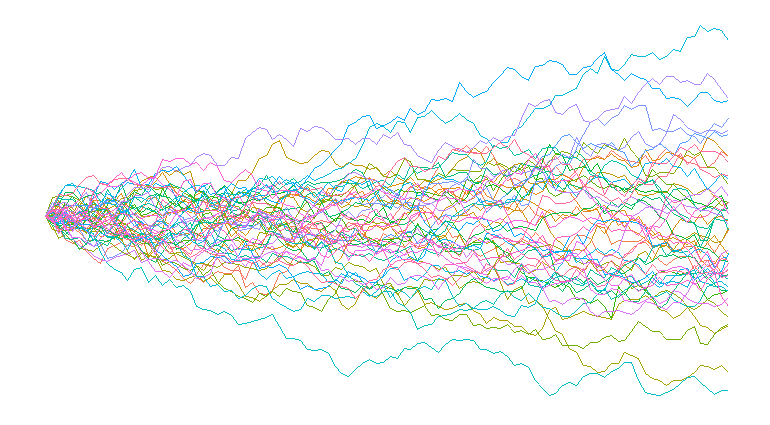
\includegraphics[width=0.666\linewidth]{GBM.png}
\end{center}
\vspace{-2.333ex}


\pdfbookmark[1]{\refname}{ref}
\begin{thebibliography}{}
\bibitem{Karatzas-Shreve--GTM113} I.~Karatzas; S.E.~Shreve. (1998). \emph{Brownian Motion and Stochastic Calculus} (2nd ed.). Springer.
\bibitem{龚光鲁-钱敏平} 龚光鲁; 钱敏平. (2019). \emph{随机微分方程引论}（第3版）. 电子工业出版社.

\bibitem{Revuz-Yor} D.~Revuz; M.~Yor. (2005). \emph{Continuous Martingales and Brownian Motion} (3rd ed.). Springer.
\bibitem{ChungKL-Williams} K.L.~Chung; R.J.~Williams. (1990). \emph{Introduction to Stochastic Integration} (2nd ed.). Birkh\"{a}user. \\
龚光鲁. (2021). \emph{钟开莱随机积分导论}~第2版. 世界图书出版公司.

\bibitem{LeGall--GTM274} J.-F.~Le~Gall. (2016). \emph{Brownian Motion, Martingales, and Stochastic Calculus}. Springer.
%\bibitem{Stroock} D.W.~Stroock. (2018). \emph{Elements of Stochastic Calculus and Analysis}. Springer.
\bibitem{Medvegyev} P.~Medvegyev. (2007). \emph{Stochastic Integration Theory}. Oxford University Press.
%\bibitem{Kallianpur-Sundar} G.~Kallianpur; P.~Sundar. (2014). \emph{Stochastic Analysis and Diffusion Processes}. Oxford University Press.
\bibitem{Spreij@Amsterdam} P.J.C.~Spreij. {\small \url{https://staff.fnwi.uva.nl/p.j.c.spreij/onderwijs/master/si.pdf}}
\bibitem{Chafaï@PSL} D.~Chafa\"{i}. {\small \url{https://djalil.chafai.net/docs/M2/m2-stochastic-calculus-course-2020-2021.pdf}}
\bibitem{Bauerschmidt@Cambridge} R.~Bauerschmidt. {\small \url{http://www.statslab.cam.ac.uk/~rb812/teaching/sc2020}}
\bibitem{almostsuremath} G.~Lowther. {\small \url{https://almostsuremath.com/stochastic-calculus}}
\end{thebibliography}

\clearpage

\pdfbookmark[1]{\contentsname}{toc}
\tableofcontents

\vspace{-2.333ex}

%\begin{center}
%	
\includegraphics[width=0.211\linewidth]{56556948.jpg}
%\end{center}

\clearpage
\pagenumbering{arabic}
\setcounter{page}{1}


\addtocounter{section}{-1}
\section{引言 \normalfont\footnotesize (2021年9月15日+22日)}
\subsection*{什么是随机分析}
概率论归类于分析学. 比之微积分, 我们在随机分析中关心
\begin{enumerate}
	\item 随机过程的构造: 用常见过程进行线性表示
	\item 对鞅或半鞅的随机积分: 通过局部化推广
	\item 随机(偏)微分方程
	\item 非光滑分析: 局部时
	\item 鞅性质在一些变换下的不变性
\end{enumerate}

\subsection*{回顾: Brown运动, It\^{o}随机积分}
固定概率空间$(\Omega,\mathscr{F},\P)$和滤流$(\mathscr{F}_{t})_{t \ge 0}$. 以$(B_{t})_{t \ge 0}$记零初值标准Brown运动.
\begin{Thm}
若零初值随机过程$(X_{t})_{t \ge 0}$具有独立平稳增量和连续轨道, 则存在常数$\sigma$和$b$, 以及零初值标准Brown运动$(\tilde{B}_{t})_{t \ge 0}$, 使得$X_{t} = \sigma\tilde{B}_{t} + b t$, $\forall t \ge 0$.
\end{Thm}

\begin{Lem}[二次变差]
设$0 = t_{0} < t_{1} < \dots < t_{m} = T$, 则
\[ \E\big[\abs{ \tsum_{k=1}^{m}(B_{t_{k}}-B_{t_{k-1}})^{2} - T }^{2}\big] = 2 \tsum_{k=1}^{m}(t_{k}-t_{k-1})^{2} \le 2 \max\nolimits_{k}(t_{k}-t_{k-1}) \, T . \]
令分划加细$(\max_{k}(t_{k}-t_{k-1}) \to 0)$即得$L^2$收敛, 对于特定分划如$2^n$-等分$(n\to\infty)$有$\as$收敛.
\begin{Rmk}
关键在于$(B_{t}^{2}-t)_{t \ge 0}$是鞅.
\end{Rmk}
\end{Lem}
\begin{Thm}
以概率一Brown运动的轨道在任何有限区间上都不是有界变差的.
\begin{proof}
$\tsum_{k=1}^{m}(B_{t_{k}}-B_{t_{k-1}})^{2} \le \Xi \tsum_{k=1}^{m}\abs{B_{t_{k}}-B_{t_{k-1}}}$, 其中$\Xi := \max_{1 \le k \le m} \abs{B_{t_{k}}-B_{t_{k-1}}} \xrightarrow{\as} 0$.
\end{proof}
\end{Thm}

\begin{Eg}[$\int_{0}^{T} B_{t} \d B_{t}$]
令$s_{k-1} := (1-\alpha)t_{k-1} + \alpha t_{k}$, 其中$\alpha \in [0,1]$是常数, 则
\[ \tsum_{k=1}^{m} B_{s_{k-1}} (B_{t_{k}}-B_{t_{k-1}}) \xrightarrow{L^2} \tfrac{1}{2}B_{T}^{2} + (\alpha-\tfrac{1}{2})T . \]
\end{Eg}

\begin{Def}[It\^{o}积分]
可料阶梯过程$H_{t} = H_{0}\1_{\{0\}}(t) + \tsum_{k=1}^{m} H_{t_{k-1}} \1_{(t_{k-1},t_{k}]}(t)$的It\^{o}积分为
\[ \tint_{0}^{T} H_{t} \d B_{t} := \tsum_{k=1}^{m} H_{t_{k-1}} (B_{t_{k}}-B_{t_{k-1}}) . \]
一般的循序可测过程的It\^{o}积分为其可料阶梯过程近似的It\^{o}积分的$L^2$极限.
\end{Def}
\begin{Prop}
It\^{o}积分满足: 可测、线性、可加.
\end{Prop}

\begin{Prop}
设$(H_{t})_{t \ge 0}$是循序可测过程. 在适当的可积性条件下: 
\begin{itemize}
\item $\big( \int_{0}^{t} H_{s} \d B_{s} \big)_{t \ge 0}$是连续鞅, 特别地有: 
$\E\int_{0}^{t} H_{s} \d B_{s} = 0$.
\item $\big( (\int_{0}^{t} H_{s} \d B_{s})^{2} - \int_{0}^{t} H_{s}^{2} \d s \big)_{t \ge 0}$是连续鞅, 特别地有\textbf{It\^{o}等距}: 
$\E\big[(\int_{0}^{t} H_{s} \d B_{s})^{2}\big] = \E\int_{0}^{t} H_{s}^{2} \d s$.
\item $\big( \e^{\int_{0}^{t} H_{s} \d B_{s} - \frac{1}{2}\int_{0}^{t} H_{s}^{2} \d s} \big)_{t \ge 0}$是连续鞅, 特别地有: 
$\E\,\e^{\int_{0}^{t} H_{s} \d B_{s}} = \E\,\e^{\frac{1}{2}\int_{0}^{t} H_{s}^{2} \d s}$.
\end{itemize}
\end{Prop}


\subsection*{随机微分方程}
\begin{Thm}
给定Brown运动$(B_{t})_{t \ge 0}$, 考察$\d X_{t} = \sigma(t,X_{t}) \d B_{t} + b(t,X_{t}) \d t$. 若$\sigma$和$b$满足Lipschitz条件, 则存在唯一的局部解$(X_{t})_{t \in [0,\epsilon]}$; 进一步地, 若$\sigma$和$b$还满足线性增长条件, 则有全局解$(X_{t})_{t \ge 0}$.
\end{Thm}
\begin{Rmk}
与此相对地, 给定随机过程$(X_{t})_{t \ge 0}$, 我们关心如何简单地表示$X_t$, 比如能否构造Brown运动$(B_{t})_{t \ge 0}$使得$\d X_{t} = \sigma(t,X_{t}) \d B_{t} + b(t,X_{t}) \d t$.
\end{Rmk}



\section{基本概念 \normalfont\footnotesize (2021年9月22日)}
\begin{Def}[随机过程相等]
两个随机过程$(X_{t})$和$(Y_{t})$
\begin{itemize}
	\item \textbf{(有限维)分布相同}, 若$(X_{t_1},\dots,X_{t_m}) \stackrel{d}{=} (Y_{t_1},\dots,Y_{t_m})$, $\forall t_{1} < \dots < t_{m}$, $\forall m \ge 1$;
	\item 互为\textbf{修正}, 若$\P\{ X_{t} = Y_{t} \} = 1$, $\forall t$;
	\item \textbf{不可区分}, 若$\P\{ X_{t} = Y_{t} , \ \forall t \} = 1$.
\end{itemize}
\end{Def}
\begin{Rmk}
不可区分的随机过程必然互为修正. 互为修正的随机过程必然有相同的有限维分布.
\end{Rmk}

\begin{Eg}
设$(B_{t})_{t \ge 0}$是零初值标准Brown运动. 令$\tilde{B}_{t} := B_{t}\1_{[t\neq\tau]}$, 其中$\tau := \inf\{ t \ge 0 : \abs{B_{t}} = 1 \}$. 易得$(\tilde{B}_{t})_{t \ge 0}$和$(B_{t})_{t \ge 0}$互为修正, 但不是不可区分的.
\end{Eg}

\begin{Eg}
记$\gamma(\d x) := \frac{1}{\sqrt{2\pi}}\e^{-x^{2}/2} \d x$和$p_{t}(x, \d y) := \gamma(\d\frac{y-x}{\sqrt{t}})$.
\begin{itemize}
	\item 在$(\R^{\infty},\mathscr{B}_{\R}^{\infty},\gamma^{\infty})$上定义$\xi_{n}(\omega_{1},\omega_{2},\dots) = \omega_{n}$, 则$\xi_{n} \iidsim \N(0,1)$. 令$X_{t} := \sum_{n=1}^{\infty} \sqrt{2} \frac{\sin((n-\frac{1}{2})\pi t)}{(n-\frac{1}{2})\pi} \xi_{n}$, 则$(X_{t})_{t \in [0,1]}$与零初值标准Brown运动有限维分布相同. \hfill\normalfont (Karhunen--Lo\`{e}ve)
	\item 在$C([0,1];\R)$上配备一致范数$\norm{w} := \max_{t \in [0,1]} \abs{w(t)}$, 诱导拓扑及Borel代数. 存在概率测度$\P^W$适合$\P^{W}\{ w \in C([0,1];\R) : w(t_{1}) \in A_{1} , \dots , w(t_{m}) \in A_{m} \} = \int_{A_{1} \times \dots \times A_{m}} \prod_{k=1}^{m} p_{t_{k}-t_{k-1}}(x_{k-1}, \d x_{k})$, $\forall 0 = t_{0} < t_{1} < \dots < t_{m} \le 1$, $\forall A_{1},\dots,A_{m} \in \mathscr{B}_{\R}$, $\forall m \ge 1$, 其中$x_{0} = 0$. 令$W_{t}(w) := w(t)$, 则$(W_{t})_{t \in [0,1]}$是$C([0,1];\R)$上的零初值标准Brown运动. \hfill\normalfont (Wiener)
\end{itemize}
不同概率空间上的随机过程可以有相同的有限维分布, 也只能在分布上进行比较.
\end{Eg}


\begin{Def}[通常条件]
概率空间$(\Omega,\mathscr{F},\P)$上的滤流$(\mathscr{F}_{t})_{t \ge 0}$的\textbf{通常条件}指的是
\begin{itemize}
	\item (完备) 所有$\P$-零测集都在$\mathscr{F}_{0}$中,
	\item (右连续) $\mathscr{F}_{t} = \mathscr{F}_{t}^{+} := \bigcap_{u > t} \mathscr{F}_{u}$, $\forall t$.
\end{itemize}
\end{Def}
\begin{Rmk}
滤流$(\mathscr{F}_{t}^{+})_{t \ge 0}$总是右连续的.
\end{Rmk}


\begin{Def}[停时]
给定滤流$(\mathscr{F}_{t})_{t \ge 0}$, 非负随机变量$\tau$为
\begin{itemize}
	\item \textbf{可选时}, 若$\{ \tau < t \} \in \mathscr{F}_{t}$, $\forall t$;
	\item \textbf{停时}, 若$\{ \tau \le t \} \in \mathscr{F}_{t}$, $\forall t$.
\end{itemize}
\end{Def}

\begin{Prop}
停时总是可选时. 如果滤流右连续, 那么可选时是停时.
\begin{proof}
一方面, $\{ \tau < t \} = \bigcup_{n=1}^{\infty} \{ \tau \le t - \frac{1}{n} \}$. 
另一方面, $\{ \tau \le t \} = \bigcap_{n=1}^{\infty} \{ \tau < t + \frac{1}{n} \}$. 
\end{proof}
\end{Prop}


\begin{Ex}[首中时, \cite{Karatzas-Shreve--GTM113}:~1.2.6,~1.2.7]
设$(\xi_{t})_{t \ge 0}$是定义在带滤流$(\mathscr{F}_{t})_{t \ge 0}$的概率空间上取值于完备可分度量空间$(S,d)$的轨道右连续的随机过程. 证明: 若$G$是开集, 则$\tau := \inf\{ t > 0 : \xi_{t} \in G \}$是可选时; 若$(\xi_{t})$的轨道是连续的, $F$是闭集, 则$\tau' := \inf\{ t > 0 : \xi_{t} \in F \}$是停时.
\begin{Prf}
利用轨道右连续性, $\{ \tau < t \} = \bigcup_{r \in (0,t)\cap\Q} \{ \xi_{r} \in G \} \in \mathscr{F}_{t}$. 令$\tau_{n} := \inf\{ t > 0 : \xi_{t} \in G_{n} \}$, 其中$G_{n} := \{ x \in S : d(x,F) < \frac{1}{n} \}$是开集. 设$(\xi_{t})_{t \ge 0}$轨道连续, 往证$\{ \tau' \le t \} = \bigcap_{n=1}^{\infty} \{ \tau_{n} < t \}$. 由$G_{1} \supset G_{2} \supset \dots \supset F$可得$\tau_{n} \nearrow \tau^{*} \le \tau'$. 在$\{ \tau^{*} < \infty \} \subset \{ \tau' < \infty \}$上, 有$\xi_{\tau^{*}} \in \bigcap_{n=1}^{\infty} \cl{G_{n}} = F$, 从而$\tau' \le \tau^{*}$. 在$\{ \tau_{n} < \infty \} \subset \{ \tau^{*} < \infty \}$上, 有$\xi_{\tau_{n}} \in \partial G_{n} = \{ x \in S : d(x,F) = \frac{1}{n} \}$, 从而$\tau_{n} < \tau' = \tau^{*}$.
\end{Prf}
\end{Ex}


设$X = (X_{t})_{t \ge 0}$是轨道$\as$右连左极的随机过程, $A := \{ X \,\text{在}\, [0,t_{0}) \,\text{上}\text{连续} \}$. 证明:
\begin{Ex}[\cite{Karatzas-Shreve--GTM113}~1.1.7]\label{Ex:measurability}
如果$X$的每条轨道都是右连左极的, 那么$A \in \mathscr{F}_{t_0}^{X} := \sigma(X_{s} : 0 \le s \le t_{0})$.
\begin{Prf}\vspace{-2.3ex}
\[\begin{aligned}
A^{\complement} &= \bigcup_{t \in (0,t_{0})} \{ \lim_{\Q \owns q \nearrow t} X_{q} \neq \lim_{\Q \owns r \searrow t} X_{r} \} \\
&= \bigcup_{t \in (0,t_{0})} \bigcup_{n\ge 1} \{ \lim_{\Q \owns q \nearrow t} \lim_{\Q \owns r \searrow t} \abs{X_{q}-X_{r}} > \tfrac{1}{n} \} \\
&\subset \bigcup_{n\ge 1} \bigcap_{m\ge 1} \bigcup_{q,r \in (0,t_{0})\cap\Q : \abs{q-r}<\frac{1}{m}} \{ \abs{X_{q}-X_{r}} > \tfrac{1}{n} \} \quad \in \mathscr{F}_{t_0}^{X} \\
&\subset \bigcup_{n\ge 1} \bigcup_{t \in [0,t_{0}]} \bigcup_{(0,t_{0}) \owns q_{j} \to t} \bigcup_{(0,t_{0}) \owns r_{j} \to t} \bigcap_{j\ge 1} \{ \abs{X_{q_{j}}-X_{r_{j}}} > \tfrac{1}{n} \} \\
&= \bigcup_{t \in [0,t_{0}]} \{ \limsup_{(0,t_{0}) \owns s \to t} X_{s} \neq \liminf_{(0,t_{0}) \owns s \to t} X_{s} \} \ = A^{\complement} .
\end{aligned}\vspace{-3.7ex}\]
\end{Prf}
\end{Ex}
\begin{Ex}[\cite{Karatzas-Shreve--GTM113}~1.1.8]
可能有$A \notin \mathscr{F}_{t_0}^{X}$. 如果$X$适应于滤流$(\mathscr{F}_{t})_{t \ge 0}$, 且$\mathscr{F}_{t_0}$完备, 那么$A \in \mathscr{F}_{t_0}$.
\begin{Prf}
令$C := \{ X \,\text{右连左极} \}$. \par
在$(\Omega,\mathscr{F}) = (\R,\mathscr{B}_{\R})$上定义$\P(B) := \int_{0}^{1} \1_{B}(\omega) \d\omega$, 考察$X_{t}(\omega) = \1_{[t=\omega>1]}$, 可见$C^{\complement} = (1,\infty)$是$\P$-零测集. 置$t_{0} = 2$, 则有$A^{\complement} = (1,2)$, 而$\mathscr{F}_{t_0}^{X} = \sigma\big(\big\{ \{t\} : 1 < t \le 2 \big\}\big)$只含至多可数集及其补集. \par
类似习题\ref{Ex:measurability}可得$A^{\complement} \cap C = C \cap \bigcup_{n\ge 1} \bigcap_{m\ge 1} \bigcup_{q,r \in (0,t_{0})\cap\Q : \abs{q-r}<\frac{1}{m}} \{ \abs{X_{q}-X_{r}} > \tfrac{1}{n} \}$. 若$\mathscr{F}_{t_0}$完备, 则$C^{\complement}$和$C$都在$\mathscr{F}_{t_0}$中. 若还有$\mathscr{F}_{t_0}^{X} \subset \mathscr{F}_{t_0}$, 则$A^{\complement} \cap C \in \mathscr{F}_{t_0}$, 进而$A = (A^{\complement} \cap C)^{\complement} \cap C \in \mathscr{F}_{t_0}$.
\end{Prf}
\end{Ex}



\section{随机过程 \normalfont\footnotesize (2021年9月24日)}
固定概率空间$(\Omega,\mathscr{F},\P)$和满足通常条件的滤流$(\mathscr{F}_{t})_{t \ge 0}$.
\begin{Def}[可测性]
设$X = (X_{t})_{t \ge 0}$是取值于可测空间$(S,\Sigma)$的随机过程. 称$X$
\begin{itemize}
	\item \textbf{可测}, 若$(t,\omega) \in [0,\infty)\times\Omega \mapsto X_{t}(\omega) \in S$是$(\mathscr{B}_{[0,\infty)}\otimes\mathscr{F})/\Sigma$可测映射;
	\item \textbf{适应}, 若$\omega \in \Omega \mapsto X_{t}(\omega) \in S$是$\mathscr{F}_{t}/\Sigma$可测映射, $\forall t$;
	\item \textbf{循序可测}, 若$(s,\omega) \in [0,t]\times\Omega \mapsto X_{s}(\omega) \in S$是$(\mathscr{B}_{[0,t]}\otimes\mathscr{F}_{t})/\Sigma$可测映射, $\forall t$;
	\item \textbf{可料}, 若$(t,\omega) \in [0,\infty)\times\Omega \mapsto X_{t}(\omega) \in S$是$\mathscr{P}/\Sigma$可测映射, 其中\par\hspace{1em}
	$\mathscr{P} := \sigma\big( \{ [0,\infty)\times A : A\in\mathscr{F}_{0} \} \cup \{ (s,u]\times A : A\in\mathscr{F}_{s} ,\, 0<s<u<\infty \} \big)$为\textbf{可料$\sigma$-代数}.
\end{itemize}
\end{Def}

\begin{Prop}
可测适应随机过程必然存在循序可测修正.
\end{Prop}

\begin{Prop}
轨道右连续的适应随机过程必然循序可测.
\end{Prop}

\begin{Prop}
可料随机过程必然循序可测.
\end{Prop}

\begin{Prop}\label{Prop:predictable}
$\mathscr{P} = \sigma(\text{左连续}\text{适应}\text{随机过程}) = \sigma(\text{左连右极}\text{适应}\text{随机过程}) = \sigma(\text{连续}\text{适应}\text{随机过程})$.
\end{Prop}

\begin{Def}[平方可积鞅]
设$M = (M_{t})$是$(\mathscr{F}_{t})$-鞅. 称$M$\textbf{平方可积}, 若$M_{t} \in L^{2}(\P)$, $\forall t$. 记\begin{itemize}
	\item $\mathcal{M}^{2} := \{ \text{平方可积}\text{的}\text{零初值}\text{右连左极}\,(\mathscr{F}_{t})_{t \ge 0}\text{-鞅} \}$, $\mathcal{M}^{2}_{\mathrm{cts}} := \{ M\in\mathcal{M}^{2} : t \mapsto M_{t} \,\text{连续} \}$,
	\item $\mathcal{M}^{2}_{T} := \{ \text{平方可积}\text{的}\text{零初值}\text{右连左极}\,(\mathscr{F}_{t})_{t \in [0,T]}\text{-鞅} \}$, $\mathcal{M}^{2}_{T,\mathrm{cts}} := \{ M\in\mathcal{M}^{2}_{T} : t \mapsto M_{t} \,\text{连续} \}$,
	\item $\mathcal{M}^{2}_{\infty} := \{ M\in\mathcal{M}^{2} : \sup_{t \ge 0} \E M_{t}^{2} < \infty \}$, $\mathcal{M}^{2}_{\infty,\mathrm{cts}} := \mathcal{M}^{2}_{\infty}\cap\mathcal{M}^{2}_{\mathrm{cts}}$.
\end{itemize}
称$\mathcal{M}^{2}_{\infty}$中的元素为\textbf{一致平方可积鞅}.
\end{Def}

\begin{Prop}
$\mathcal{M}^{2}_{\infty} = \{ (\E[M_{\infty}|\mathscr{F}_{t}])_{t \ge 0} : M_{\infty} \in L^{2}(\P) ,\, \E[M_{\infty}|\mathscr{F}_{0}] = 0 \}$.
\end{Prop}

\begin{Thm}[\href{https://almostsuremath.com/2011/12/30/the-doob-meyer-decomposition/}{Doob--Meyer分解}]
设$X = (X_{t})_{t \ge 0}$是右连左极下鞅. 若$X$满足\href{https://almostsure.wordpress.com/2009/12/22/class-d-processes/}{一定条件}, 则存在唯一的鞅$M = (M_{t})_{t \ge 0}$和可料可积零初值右连续增过程$A = (A_{t})_{t \ge 0}$, 使得$X = M+A$.
\begin{Def}[补偿子]
上述分解中, $A$称为$X$的\textbf{补偿子}.
\end{Def}
\end{Thm}

\begin{Eg}
速率$\lambda$的Poisson过程的补偿子为$(\lambda t)_{t \ge 0}$.
\end{Eg}

\begin{Def}[尖括号过程]
对于$M = (M_{t})_{t \ge 0} \in \mathcal{M}^{2}$, 称$(M_{t}^{2})_{t \ge 0}$的补偿子为$M$的\textbf{特征}, 记作$\agp{M}$.
\end{Def}

\begin{Eg}
设$B = (B_{t})_{t \ge 0}$是标准Brown运动, 则$\agp{B}_{t} = t$.
\end{Eg}

\begin{Thm}\label{Thm:<M>=[M]_for_M_cts}
设$M \in \mathcal{M}^{2}_{\mathrm{cts}}$, 则$t \mapsto \agp{M}_{t}$连续, 并且$\agp{M}_{t}$是$[0,t]$上$M$的\textbf{二次变差}的依概率极限.
\end{Thm}


\begin{Ex}
证明: $(M,N) \mapsto \E M_{T}N_{T}$使$\mathcal{M}^{2}_{T}$成为Hilbert空间, 并且$\mathcal{M}^{2}_{T,\mathrm{cts}}$是$\mathcal{M}^{2}_{T}$的闭子空间.
\begin{Prf}
不难验证内积性质, 下面考虑完备性. 任取$M^{(n)} \in \mathcal{M}^{2}_{T}$适合$M^{(m)}_{T}-M^{(n)}_{T} \xrightarrow[m,n \to \infty]{L^{2}(\P)} 0$. 利用Doob极大不等式, $\sup_{t \in [0,T]} \abs{M^{(m)}_{t}-M^{(n)}_{t}} \xrightarrow[m,n \to \infty]{L^{2}(\P)} 0$, 进而存在$n_{1} < n_{2} < \dots$和$\P$-零测集$D$使得$\big\{ \sup_{t \in [0,T]} \abs{M^{(n_{j})}_{t}-M^{(n_{k})}_{t}} \xrightarrow[j,k \to \infty]{} 0 \big\} \supset D^{\complement}$. 令$M_{t} := \lim_{k\to\infty} M^{(n_{k})}_{t} \1_{D^\complement}$, 则$M = (M_{t})_{t \in [0,T]}$保持轨道连续性, 因为在$D^\complement$上, $\sup_{u \in [0,T]} \abs{M_{u}-M_{u}^{(n_{k})}} \le \liminf_{j\to\infty} \sup_{t \in [0,T]} \abs{M_{t}^{(n_{j})}-M_{t}^{(n_{k})}} \xrightarrow[k\to\infty]{} 0$, 而
\[ \abs{M_{t}-M_{s}} \le \abs{M_{t}-M_{t}^{(n_{k})}} + \abs{M_{t}^{(n_{k})}-M_{s}^{(n_{k})}} + \abs{M_{s}^{(n_{k})}-M_{s}} \le \abs{M_{t}^{(n_{k})}-M_{s}^{(n_{k})}} + 2 \sup\nolimits_{u} \abs{M_{u}-M_{u}^{(n_{k})}} . \]
对任意$t \in [0,T]$有$L^{2}(\P)\text{-}\lim_{n\to\infty}M^{(n)}_{t} \stackrel{\as}{=} \P\text{-}\lim_{k\to\infty}M^{(n_{k})}_{t} = M_{t}$, 这还表明$M$是平方可积鞅, 因为只要$s \le t$就有$\E M_{t}\1_{A} = \lim_{n\to\infty} \E M_{t}^{(n)}\1_{A} = \lim_{n\to\infty} \E M_{s}^{(n)}\1_{A} = \E M_{s}\1_{A}$, $\forall A \in \mathscr{F}_{s}$.
\end{Prf}
\end{Ex}


\begin{Ex}\label{Ex:Poisson_process_Doob-Meyer}
设$N = (N_{t})_{t \ge 0}$是速率参数为$\lambda$的Poisson过程, $\mathscr{F}_{t} = \mathscr{F}_{t}^{N} := \sigma(N_{s} : s \le t)$.
\begin{enumerate}
\setlength{\itemsep}{0ex}
	\item 证明$(N_{t} - \lambda t)_{t \ge 0}$是$(\mathscr{F}_{t})_{t \ge 0}$-鞅;
\begin{Prf}
根据增量性质可得$\E[N_{t}-N_{s}|\mathscr{F}_{s}] = \lambda (t-s)$, $\forall t > s$.
\end{Prf}
	\item 求$((N_{t} - \lambda t)^{2})_{t \ge 0}$的Doob--Meyer分解;
\begin{Soln}
记$\tilde{N}_{t} := N_{t} - \lambda t$. 由$\tilde{N}_{t}^{2} = \tilde{N}_{s}^{2} + 2 \tilde{N}_{s} (\tilde{N}_{t}-\tilde{N}_{s}) + (\tilde{N}_{t}-\tilde{N}_{s})^{2}$, 可得
\[ \E[\tilde{N}_{t}^{2}|\mathscr{F}_{s}] - \tilde{N}_{s}^{2} = 2 \tilde{N}_{s} \E(\tilde{N}_{t}-\tilde{N}_{s}) + \Var(\tilde{N}_{t}-\tilde{N}_{s}) = \Var(N_{t}-N_{s}) = \lambda (t-s) , \ \forall t > s . \]
于是$\agp{\tilde{N}}_{t} = \lambda t$, 即$(\tilde{N}_{t}^{2} - \lambda t)_{t \ge 0}$是$(\mathscr{F}_{t})_{t \ge 0}$-鞅.
\end{Soln}
	\item 设$X = (X_{n})_{n \ge 0}$是i.i.d.随机变量序列, $X_{0}$可积, 且$N$与$X$独立. 令$Y_{t} := \sum_{n=0}^{N_t} X_{n}$, 则$Y = (Y_{t})_{t \ge 0}$称为\textbf{复合Poisson过程}. 求$Y$的Doob--Meyer分解.
\begin{Soln}
令$\mathscr{G}_{t} := \mathscr{F}_{t}^{N} \vee \sigma(X_{n\wedge N_{t}} : n \ge 0)$, 则$Y$适应于$(\mathscr{G}_{t})_{t \ge 0}$. 我们有$Y_{t}-Y_{s}|\mathscr{G}_{s} \stackrel{d}{=} \sum_{n=1}^{N_{t}-N_{s}} X_{n}'$, 其中$(X_{n}')_{n \ge 0}$是独立于$\mathscr{G}_{t}$的$X$的同分布拷贝, 从而$\E[Y_{t}-Y_{s}|\mathscr{G}_{s}] = \E\sum_{n=1}^{N_{t}-N_{s}} X_{n}' = \lambda (t-s) \mu$, $\forall t > s$, 其中$\mu := \E X_{0}$. 因此, $Y$的补偿子为$(\mu \lambda t)_{t \ge 0}$, 即$(Y_{t} - \mu \lambda t)_{t \ge 0}$是$(\mathscr{G}_{t})_{t \ge 0}$-鞅.
\end{Soln}
\end{enumerate}
\end{Ex}



\section{随机过程·续 \normalfont\footnotesize (2021年9月27日)}
\begin{Def}[互特征]
$\agp{M,N} := \frac{1}{4}\big( \agp{M+N} - \agp{M-N} \big)$称为$M,N \in \mathcal{M}^2$的\textbf{互特征}.
\begin{Rmk}
$\agp{M,N} = \frac{1}{2}\big( \agp{M+N} - \agp{M} - \agp{N} \big)$.
\end{Rmk}
\end{Def}

\begin{Prop}
$(M_{t}N_{t}-\agp{M,N}_{t})_{t \ge 0}$是鞅, $\forall M,N \in \mathcal{M}^2$.
\end{Prop}

\begin{Prop}
$(M,N) \mapsto \agp{M,N}$是$\mathcal{M}^{2}$上的正定对称双线性映射.
\end{Prop}

\begin{Def}[生成元]
半群$(P_{t})_{t \ge 0}$的\textbf{生成元}为$\mathsf{A} := \frac{\d}{\d t}\big|_{t=0+} \mathsf{P}_{t}$, 其中$\mathsf{P}_{t}f(x) := \int P_{t}(x,\d y) f(y)$, $f \in C_{b}$.
\end{Def}

\begin{Prop}
$\mathsf{A}\mathsf{P}_{t} = \frac{\d}{\d t} \mathsf{P}_{t} = \mathsf{P}_{t}\mathsf{A}$, $\forall t \ge 0$.
\end{Prop}

\begin{Eg}
转移速率矩阵为$Q$的时齐连续时间Markov链的生成元为$\mathsf{A}f(x) = \sum_{y} Q(x,y) f(y)$, $f \in C_{b}$.
\end{Eg}

\begin{Thm}
设$(X_{t})_{t \ge 0}$是生成元为$\mathsf{A}$的时齐Markov过程, 则$\big( f(X_{t}) - \int_{0}^{t} \mathsf{A}f(X_{s}) \d s \big)_{t \ge 0}$是鞅, $\forall f \in C_{b}$.
\begin{proof}
记Markov转移半群为$(P_{t})_{t \ge 0}$, 则$\E[f(X_{t+u})|\mathscr{F}_{t}] = \mathsf{P}_{u}f(X_{t})$, $\forall t, u \ge 0$. 利用$\frac{\d}{\d u} \mathsf{P}_{u} = \mathsf{P}_{u}\mathsf{A}$, 可得$\mathsf{P}_{u}f(X_{t}) - f(X_{t}) = \int_{0}^{u} \mathsf{P}_{v}\mathsf{A}f(X_{t}) \d v 
= \int_{0}^{u} \E[\mathsf{A}f(X_{t+v})|\mathscr{F}_{t}] \d v 
= \E[ \int_{0}^{u} \mathsf{A}f(X_{t+v}) \d v |\mathscr{F}_{t}]$.
\end{proof}
\end{Thm}

\begin{Def}[随机测度]
可测空间$(S,\Sigma)$上的\textbf{随机测度}指的是满足可数可加性的映射$\Lambda : B \in \Sigma \mapsto \Lambda(B) \in \{ \text{取值于}\,[0,\infty]\,\text{的}\text{随机变量} \}$.
\end{Def}

\begin{Eg}
存在$(\R^{d},\mathscr{B}_{\R}^{d})$上的随机测度$\Lambda$, 称为强度$\lambda$的Poisson点过程, 适合$\Lambda(B) \sim \mathrm{Poisson}(\lambda\abs{B})$, 并且只要$B_{1},\dots,B_{k}$两两不交就有$\Lambda(B_{1}),\dots,\Lambda(B_{k})$独立.
\end{Eg}

\begin{Def}[计数过程]
对应于$[0,\infty)$上的非负整数值随机测度$\Lambda$的\textbf{计数过程}为$N_{t} := \Lambda([0,t])$, $t \ge 0$.
\end{Def}

\begin{Eg}
非负随机变量$X_{1},X_{2},\dots$决定更新过程$N_{t} := \sup\{ n : \sum_{i=1}^{n} X_{i} \le t \}$, $t \ge 0$.
\end{Eg}

\begin{Def}[简单计数过程]
关于滤流$(\mathscr{F}_{t})_{t \ge 0}$适应的计数过程$N = (N_{t})_{t \ge 0}$称为\textbf{简单的}, 若存在循序可测随机过程$\lambda = (\lambda_{s})_{s \ge 0}$和一列有限停时$\tau_{n} \to \infty$, 使得$\E[N_{u\wedge\tau_{n}}-N_{t\wedge\tau_{n}}|\mathscr{F}_{t}] = \E[\int_{t\wedge\tau_{n}}^{u\wedge\tau_{n}} \lambda_{s} \d s |\mathscr{F}_{t}]$, $\forall u \ge t \ge 0$, $\forall n$, 其中$\lambda$称为\textbf{随机速率}. 换言之, $\big( N_{t} - \int_{0}^{t} \lambda_{s} \d s \big)_{t \ge 0}$是$(\mathscr{F}_{t})_{t \ge 0}$-\emph{局部鞅}.
\end{Def}


\begin{Ex}[\cite{Karatzas-Shreve--GTM113}~1.5.7]
设$M,N \in \mathcal{M}^2$. 证明:
\begin{enumerate}
\setlength{\itemsep}{0ex}
	\item $\agp{M,N}_{t}^{2} \le \agp{M}_{t} \agp{N}_{t}$, $\forall t \ge 0$.
\begin{Prf}
只需考察$\alpha \in \R \mapsto \agp{M}_{t}\alpha^{2} + 2\agp{M,N}_{t}\alpha + \agp{N}_{t} = \agp{\alpha M + N}_{t} \ge 0$的判别式.
\end{Prf}
	\item 设$V_{t}$是$[0,t] \owns u \mapsto \agp{M,N}_{u}$的全变差, $t > s$, 则$V_{t}-V_{s} \le \frac{1}{2}\big( \agp{M}_{t}-\agp{M}_{s} + \agp{N}_{t}-\agp{N}_{s} \big)$.
\begin{Prf}
由于$A := \frac{1}{2}(\agp{M}+\agp{N})$是增过程, 只需$\abs{\agp{M,N}_{t}-\agp{M,N}_{s}} \le A_{t}-A_{s}$, $\forall t > s$. 不妨置$s = 0$, 此时易得$\pm \agp{M,N}_{t} \le A_{t} \iff \agp{M \mp N}_{t} \ge 0$.
\end{Prf}
\end{enumerate}
\end{Ex}


\begin{Ex}
设$X = (X_{t})_{t \ge 0}$是一个单生过程, 即其状态空间为$\mathbb{Z}_{+} := \{0,1,2,\cdots\}$, 转移速率矩阵$Q$形如$Q(x,y) := \lambda(x)\1_{[y=x+1]} -\lambda(x)\1_{[y=x]}$. 进一步假定$\sum_{x=0}^{\infty} \frac{1}{\lambda(x)} = \infty$, 即$X$非爆炸. 求$X$的Doob--Meyer分解并验证.
\begin{Soln}
作为习题\ref{Ex:Doob-Meyer_Markov}的特例, $\big( X_{t} - \int_{0}^{t} \lambda(X_{s}) \d s \big)_{t \ge 0}$是鞅.
\end{Soln}
\end{Ex}
\begin{Ex}\label{Ex:Doob-Meyer_Markov}
设$X = (X_{t})_{t \ge 0}$是一个取值于$\mathbb{Z}_{+} := \{0,1,2,\cdots\}$的连续时间Markov链, 转移速率矩阵$Q$使得$X$非爆炸. 任取$f : \mathbb{Z}_{+} \to \R$适合$\E\abs{f(X_{t})} < \infty$, $\forall t \ge 0$. 求$f(X) = (f(X_{t}))_{t \ge 0}$的Doob--Meyer分解并验证.
\begin{Soln}
断言$M := \big( f(X_{t}) - \int_{0}^{t} \sum_{y} Q(X_{s},y) f(y) \d s \big)_{t \ge 0}$是鞅. 任取$u > t$, 有
\[ \tfrac{\d}{\d u} \E[f(X_{u})|\mathscr{F}_{t}] = \tfrac{\d}{\d h} \big|_{h=0+} \E\big[ \E[f(X_{u+h})|\mathscr{F}_{u}] \big| \mathscr{F}_{t} \big] = \E\big[ \tfrac{\d}{\d h} \big|_{h=0+} \E[f(X_{u+h})|\mathscr{F}_{u}] \big| \mathscr{F}_{t} \big] , \]
其中$\tfrac{\d}{\d h} \big|_{h=0+} \E[f(X_{u+h})|\mathscr{F}_{u}] = \sum_{y} Q(X_{u},y) f(y)$. 即得$\tfrac{\d}{\d u} \E[M_{u}|\mathscr{F}_{t}] = 0$, 进而$\E[M_{u}|\mathscr{F}_{t}] = M_{t}$.
\end{Soln}
\end{Ex}


\begin{Ex}
设$X_{1},X_{2},\dots$是i.i.d.随机变量, $\P\{X_{1}>0\} = 1$. 令$T_{n} := \sum_{i=1}^{n} X_{i}$和$N_{t} := \sum_{n=1}^{\infty} \1_{\{T_{n} \le t\}}$. 求$N = (N_{t})_{t \ge 0}$的Doob--Meyer分解并验证. 特别地, 考虑$X_{1} = 1 ~\as$的情况.
\begin{Soln}
令$\mathscr{G}_{t} := \mathscr{F}_{t}^{N} \vee \sigma( T_{n}\wedge t : n \ge 0)$, 则$N$适应于$(\mathscr{G}_{t})_{t \ge 0}$. 记$F := \P\{ X_{1} \le \bm{\cdot} \}$的$n$次卷积为$F^{*n}$. 任取$t > s$, 有$\P( T_{n}\le t \,|\,\mathscr{G}_{s}) = \1_{\{n \le N_{s}\}} + \1_{\{n > N_{s}\}} G_{n}(t;s) / [1-F(s-T_{N_{s}})]$, 其中
\[ G_{n}(t;s) := F^{*(n-N_{s})}(t-T_{N_{s}}) - \tint_{x=0}^{s-T_{N_{s}}} F^{*(n-N_{s}-1)}(t-T_{N_{s}}-x) \d F(x) , \]
从而$\E[N_{t}|\mathscr{G}_{s}]-N_{s} = \tsum_{n=1}^{\infty} \1_{\{n>N_{s}\}} G_{n}(t;s) / [1-F(s-T_{N_{s}})]$. 因此, $N$的补偿子为$A = (A_{t})_{t \ge 0}$, 其中
\[ A_{t} = \sum_{n=1}^{\infty} \int_{s=0}^{t} \frac{\1_{\{N_{s}<n\}}}{1-F(s-T_{N_{s}})} \d G_{n}(\bm{\cdot}\,;s) |_{s} . \]
如果(a.s.)\,$X_{1} = 1$, 那么$N_{t} = \lfloor t \rfloor$, 此时$A_{t} = \lfloor t \rfloor$.
\end{Soln}
\end{Ex}



\section{随机积分 \normalfont\footnotesize (2021年9月29日)}
固定$M = (M_{t})_{t \ge 0} \in \mathcal{M}^{2}_{\mathrm{cts}}$, 定义测度
\[ \mu_{M}(A) := \tint_{\Omega} \tint_{t=0}^{\infty} \1_{A}(t,\omega) \d\agp{M}_{t}(\omega) \d\P(\omega) , \quad A \in \mathscr{B}_{[0,\infty)} \otimes \mathscr{F} . \]

\begin{Def}
两个可测且适应的过程$X$和$Y$当作\emph{等价的}, 若$\mu_{M}\{ (t,\omega) : X_{t}(\omega) \neq Y_{t}(\omega) \} = 0$.
\end{Def}
\begin{Rmk}
在$\mu_{M}$下等价和互为修正是没有蕴涵关系的, 因为$\mu_{M}$涉及的重积分有顺序.
\end{Rmk}

\begin{Def}
$\mathcal{L}^{*}(M) := \bigcap_{T \in (0,\infty)} \mathcal{L}_{T}^{*}(M)$, 
$\mathcal{L}_{T}^{*}(M) := \{ \text{循序可测}\,(X_{t})_{t \ge 0} : \E\tint_{t=0}^{T} X_{t}^{2} \d\agp{M}_{t} < \infty \}/\xlongequal{\mu_{M}\text{-}\textrm{a.e.}}$.
\end{Def}

\begin{Prop}
范数$\norm{X}_{\mathcal{L}_{T}^{*}(M)} := \sqrt{\E\tint_{t=0}^{T} X_{t}^{2} \d\agp{M}_{t}}$使$\mathcal{L}_{T}^{*}(M)/\textrm{\normalfont 轨道}|_{(T,\infty)}$成为Hilbert空间.
\end{Prop}
\begin{Cor}
准范数$\norm{X}_{\mathcal{L}^{*}(M)} := \sum_{T=1}^{\infty} (1\wedge\norm{X}_{\mathcal{L}_{T}^{*}(M)})/2^{T}$使$\mathcal{L}^{*}(M)$成为完备度量空间.
\end{Cor}

\begin{Def}[简单过程]
随机过程$X = (X_{t})_{t \ge 0}$称为\textbf{简单的}, 若存在$0 = t_{0} < t_{1} < t_{2} < \dots$和一致有界的$\xi_{k} \in L^{\infty}(\mathscr{F}_{t_k},\P)$, 使
\[ X_{t} = \xi_{0} \1_{\{0\}}(t) + \tsum_{k=0}^{\infty} \xi_{k} \1_{(t_{k},t_{k+1}]}(t) , \ \forall t . \label{eq:simple_proc}\tag{$\spadesuit$}\]
所有简单过程的集合记作$\mathcal{L}_{0}$.
\end{Def}

\begin{Lem}
设$(A_{t})_{t \ge 0}$是适应的\underline{连续}\:\!增过程. 若$(X_{t})_{t \ge 0}$循序可测且$\E\tint_{t=0}^{T} X_{t}^{2} \d A_{t} < \infty$, $\forall T \in [0,\infty)$, 则存在$X^{(n)} \in \mathcal{L}_{0}$使得
\[ \E\tint_{t=0}^{T} \abs{X_{t}^{(n)}-X_{t}}^{2} \d A_{t} \xrightarrow[n\to\infty]{} 0 , \ \forall T \in [0,\infty) . \]
\end{Lem}
\begin{Thm}
$\mathcal{L}_{0}$是$\mathcal{L}^{*}(M)$的稠密子空间.
\end{Thm}

\begin{Def}[简单过程的随机积分]
\eqref{eq:simple_proc}\,$\in\mathcal{L}_{0}$关于$M$的\textbf{随机积分}为\emph{鞅变换}
\[ \tint_{0}^{t} X \d M := I^{M}_{t}(X) := \tsum_{k=0}^{\infty} \xi_{k} (M_{t_{k+1}\wedge t} - M_{t_{k}\wedge t}) , \ t \in [0,\infty) . \]
\end{Def}

\begin{Prop}
$I^{M} : X \in \mathcal{L}_{0} \mapsto I^{M}(X) := (I^{M}_{t}(X))_{t \ge 0} \in \mathcal{M}^{2}_{\mathrm{cts}}$是良定义的$\R$-线性映射.
\end{Prop}
\begin{Prop}[It\^{o}等距]
对$X \in \mathcal{L}_{0}$, 可得$\big( (\tint_{0}^{t} X \d M)^{2} - \tint_{s=0}^{t} X_{s}^{2} \d\agp{M}_{s} \big)_{t \ge 0}$是鞅. 特别地, 
\[ \norm{\tint X \d M}_{\mathcal{M}_{T}^{2}}^{2} = \E\big[ (\tint_{0}^{T} X \d M)^{2} \big] = \E\tint_{t=0}^{T} X_{t}^{2} \d\agp{M}_{t} = \norm{X}_{\mathcal{L}_{T}^{*}(M)}^{2} , \ \forall T \in [0,\infty) . \]
\end{Prop}

\begin{Def}[随机积分]
$X \in \mathcal{L}^{*}(M)$关于$M$的\textbf{随机积分}为\begin{center}
$\int X \d M := I^{M}(X) := \mathcal{M}^{2}\text{-}\lim I^{M}(X^{(n)})$, 其中$\mathcal{L}_{0} \owns X^{(n)} \xrightarrow{\mathcal{L}^{*}(M)} X ~(n\to\infty)$.
\end{center}
\end{Def}

\begin{Thm}
$I^{M} : X \in \mathcal{L}^{*}(M) \mapsto \int X \d M \in \mathcal{M}^{2}_{\mathrm{cts}}$是线性等距, 且$\agp{\int X \d M} = \big(\tint_{s=0}^{t} X_{s}^{2} \d\agp{M}_{s} \big)_{t \ge 0}$.
\end{Thm}

\begin{Prop}
若$X,Y \in \mathcal{L}^{*}(M)$是$\mu_{M}$-等价的, 则$\int X \d M$和$\int Y \d M$不可区分.
\begin{proof}
对任意$T > 0$有$\E\big[( \tint_{0}^{T} X \d M - \tint_{0}^{T} Y \d M )^{2}\big] = \norm{\tint (X-Y) \d M}_{\mathcal{M}_{T}^{2}}^{2} = \norm{X-Y}_{\mathcal{L}_{T}^{*}(M)}^{2} = 0$以及$\E\big[\!\max_{t \in [0,T]} ( \tint_{0}^{t} X \d M - \tint_{0}^{t} Y \d M )^{2}\big] \le 4 \,\E\big[( \tint_{0}^{T} X \d M - \tint_{0}^{T} Y \d M )^{2}\big]$.
\end{proof}
\end{Prop}


\begin{Ex}
设$M = (M_{t})_{t \ge 0} \in \mathcal{M}^{2}_{\mathrm{cts}}$. 证明:
\begin{enumerate}
\setlength{\itemsep}{0ex}
	\item 若$0 \le t_{0} \le t_{1} < t_{2}$, 且$\xi_{1} \in L^{\infty}(\mathscr{F}_{t_1})$, 则$\E[\xi_{1}^{2}(M_{t_2}-M_{t_1})^{2}|\mathscr{F}_{t_0}] = \E[\xi_{1}^{2}(\agp{M}_{t_2}-\agp{M}_{t_1})|\mathscr{F}_{t_0}]$.
\begin{Prf}
利用$\E[(M_{t_2}-M_{t_1})^{2}|\mathscr{F}_{t_1}] = \E[M_{t_2}^{2}|\mathscr{F}_{t_1}]-M_{t_1}^{2} = \E[\agp{M}_{t_2}|\mathscr{F}_{t_1}]-\agp{M}_{t_1}$.
\end{Prf}
	\item 对于$X \in \mathcal{L}^{*}(M)$, 有$\E[(I^{M}_{t}(X)-I^{M}_{s}(X))^{2}|\mathscr{F}_{s}] = \E[\tint_{u=s}^{t}X_{u}^{2}\d\agp{M}_{u}|\mathscr{F}_{s}] ~(\as)$, $\forall t > s$.
\begin{Prf}
因为$\mathcal{L}_{0}$在$\mathcal{L}^{*}(M)$中稠密, 只需证明$X \in \mathcal{L}_{0}$的情况, 而这由前立得.
\end{Prf}
\end{enumerate}
\end{Ex}


\begin{Ex}[\cite{Karatzas-Shreve--GTM113}~1.5.12]
设$X \in \mathcal{M}_{\mathrm{cts}}^{2}$满足$\agp{X}_{\tau} = 0 ~\as$, 其中$\tau$是停时, 证明$\P\{ X_{t\wedge\tau} = 0 , \ \forall t \} = 1$.
\begin{Prf}
任取$T > 0$, 有$\E[\max_{t \in [0,T]} X_{t\wedge\tau}^{2}] \le 4 \,\E[X_{T\wedge\tau}^{2}]$, 而$\E[X_{T\wedge\tau}^{2}] = \E\agp{X}_{T\wedge\tau} \le \E\agp{X}_{\tau} = 0$.
\end{Prf}
\end{Ex}



\section{随机积分·互特征 \normalfont\footnotesize (2021年10月11日)}
设$M,N \in \mathcal{M}^{2}_{\mathrm{cts}}$, $X \in \mathcal{L}^{*}(M)$, $Y \in \mathcal{L}^{*}(N)$, $t \ge 0$.

\begin{Thm}[Kunita--Watanabe]
$\tint_{s=0}^{t} \abs{X_{s}}\,\abs{Y_{s}} \,\abs{\d\agp{M,N}_{s}} \le \sqrt{\tint_{s=0}^{t} X_{s}^{2} \d\agp{M}_{s}} \sqrt{\tint_{s=0}^{t} Y_{s}^{2} \d\agp{N}_{s}}$.
\begin{proof}
对$\tint_{0}^{t} \d\mu$应用Cauchy--Schwarz不等式, 其中$\d\mu(s) = \abs{\d\agp{M,N}_{s}} + \d\agp{M}_{s} + \d\agp{N}_{s}$.
\end{proof}
\end{Thm}

\begin{Lem}
$\agp{\int X \d M ,\, N} = \big(\tint_{s=0}^{t} X_{s} \d\agp{M,N}_{s} \big)_{t \ge 0}$, 亦即$\d\agp{\int X \d M ,\, N}_{t} = X_{t} \d\agp{M,N}_{t}$.
\end{Lem}

\begin{Prop}
$\agp{\int X \d M ,\, \int Y \d N} = \big(\tint_{s=0}^{t} X_{s}Y_{s} \d\agp{M,N}_{s} \big)_{t \ge 0}$, 亦即$\d\agp{\int X \d M ,\, \int Y \d N}_{t} = X_{t}Y_{t} \d\agp{M,N}_{t}$.
\end{Prop}

\begin{Lem}
$\int X \d M$是方程$\agp{?,N} = \big(\tint_{s=0}^{t} X_{s} \d\agp{M,N}_{s} \big)_{t \ge 0} \ (\forall N)$在$\mathcal{M}^{2}_{\mathrm{cts}}$中的唯一解.
\hfill\normalfont (Riesz表示)
\end{Lem}

\begin{Prop}
任取停时$\tau$, 停止过程满足$(\int X \d M)^{\tau} = \big(\int_{s=0}^{t} X_{s} \1_{\{s\le\tau\}} \d M_{s}\big)_{t \ge 0} \xlongequal{\ref{Prop:dN=XdM->YdN=YXdM}} \int X^{\tau} \d (M^{\tau})$.
\begin{Rmk}
第一个等号需要$\agp{(\int X \d M)^{\tau} ,\, N} = \agp{\int X \d M ,\, N}^{\tau}$. 一般地, $\agp{M^{\tau},N} = \agp{M,N}^{\tau}$.
\end{Rmk}
\end{Prop}

\begin{Prop}\label{Prop:dN=XdM->YdN=YXdM}
若$N = \int X \d M$, 则$YX = (Y_{t}X_{t})_{t \ge 0} \in \mathcal{L}^{*}(M)$且$\int Y \d N = \int YX \d M$.
\par 换言之, 若$\d N_{t} = X_{t} \d M_{t}$, 则$Y_{t} \d N_{t} = Y_{t}X_{t} \d M_{t}$.
\end{Prop}
\begin{Cor}
$\int \xi_{0} X \d M = \xi_{0} \int X \d M$, $\forall \xi_{0} \in L^{\infty}(\mathscr{F}_{0})$.
\end{Cor}


\begin{Ex}
设$X,Y\in\mathcal{L}_{0}$, $M,N\in\mathcal{M}^{2}_{\mathrm{cts}}$. 证明$\agp{\int X \d M ,\, \int Y \d N}_{t} = \int_{s=0}^{t} X_{s}Y_{s} \d\agp{M,N}_{s}$.
\begin{Prf}
不妨$X_{\bullet} = \xi_{0} \1_{\{0\}} + \tsum_{k=0}^{\infty} \xi_{k} \1_{(t_{k},t_{k+1}]}$且$Y_{\bullet} = \eta_{0} \1_{\{0\}} + \tsum_{k=0}^{\infty} \eta_{k} \1_{(t_{k},t_{k+1}]}$, 其中$0 = t_{0} < t_{1} < \dots$, 则有$\tint X \d M = \tsum_{k=0}^{\infty} \xi_{k} (M^{t_{k+1}} - M^{t_{k}})$和$\tint Y \d N = \tsum_{k=0}^{\infty} \eta_{k} (N^{t_{k+1}} - N^{t_{k}})$. 易得
\[ \agp{\xi_{j}(M^{t_{j+1}}-M^{t_{j}}) ,\, \eta_{k}(N^{t_{k+1}}-N^{t_{k}})} = \xi_{k}\eta_{k} (\agp{M,N}^{t_{k+1}}-\agp{M,N}^{t_{k}}) \1_{[j=k]} , \ \forall j,k, \]
从而$\agp{\int X \d M ,\, \int Y \d N}_{t} = \tsum_{k=0}^{\infty} \xi_{k}\eta_{k} \int_{s=0}^{t} \1_{(t_{k},t_{k+1}]}(s) \d\agp{M,N}_{s} = \int_{s=0}^{t} X_{s}Y_{s} \d\agp{M,N}_{s}$.
\end{Prf}
\end{Ex}



\section{随机积分·局部化 \normalfont\footnotesize (2021年10月13日)}
\begin{Def}[局部可积]
适应的随机过程$X = (X_{t})_{t \ge 0}$称为\textbf{局部可积的}, 若存在一列停时$\tau_{n} \nearrow \infty ~(\as)$, 使得$X^{\tau_{n}} = (X_{t\wedge\tau_{n}})_{t \ge 0}$可积.
停时列$\{\tau_{n}\}_{n=1}^{\infty}$称为\textbf{局部化序列}, 不妨满足$\tau_{n} \le n$.
\end{Def}
\begin{Def}[局部鞅]
称右连左极(连续)的随机过程$M = (M_{t})_{t \ge 0}$为\textbf{(连续)局部(平方可积)鞅}, 若存在局部化序列$\{\tau_{n}\}_{n=1}^{\infty}$使得$M^{\tau_{n}} = (M_{t\wedge\tau_{n}})_{t \ge 0}$是(平方可积)鞅. 记\begin{itemize}
	\item $\mathcal{M}_{\mathrm{loc}} := \{ \text{零初值}\text{局部鞅} \}$, $\mathcal{M}^{2}_{\mathrm{loc}} := \{ \text{零初值}\text{局部平方可积鞅} \}$,
	\item $\mathcal{M}_{\mathrm{cts},\mathrm{loc}} := \{ \text{零初值}\text{连续}\text{局部鞅} \} = \{ \text{零初值}\text{连续}\text{局部平方可积鞅} \} \subset \mathcal{M}^{2}_{\mathrm{loc}}$.
\end{itemize}
\end{Def}

\begin{Thm}
对于$M = (M_{t})_{t \ge 0} \in \mathcal{M}^{2}_{\mathrm{loc}}$, 存在唯一的可料局部可积零初值右连续增过程$\agp{M} = (\agp{M}_{t})_{t \ge 0}$, 称为$M$的\textbf{特征}, 使得$(M_{t}^{2}-\agp{M}_{t})_{t \ge 0}$是局部鞅.
\begin{proof}
利用局部化, 可得$\agp{M}_{t} = \sum_{n=1}^{\infty} \agp{M^{\tau_{n}}}_{t} \1_{(\tau_{n-1},\tau_{n}]}(t)$, 其中$\tau_{0} := 0$.
\end{proof}
\end{Thm}
\begin{Cor}
对于$M,N \in \mathcal{M}^{2}_{\mathrm{loc}}$可以定义\textbf{互特征}\,$\agp{M,N}$, 并且$\agp{M,N}^{\tau_{n}} = \agp{M^{\tau_{n}},N^{\tau_{n}}}$. \par
特别地, $(M_{t}N_{t}-\agp{M,N}_{t})_{t \ge 0}$是局部鞅.
\end{Cor}

\begin{Def}
设$M \in \mathcal{M}_{\mathrm{cts},\mathrm{loc}}$, 令$\mathcal{L}_{\mathrm{loc}}^{*}(M) := \bigcap_{T \in (0,\infty)}\{ \text{循序可测}\,(X_{t})_{t \ge 0} : \tint_{t=0}^{T} X_{t}^{2} \d\agp{M}_{t} < \infty ~\as \}$.
\end{Def}
\begin{Def}[关于局部鞅的随机积分]
对于$M \in \mathcal{M}_{\mathrm{cts},\mathrm{loc}}$和$X = (X_{t})_{t \ge 0} \in \mathcal{L}_{\mathrm{loc}}^{*}(M)$, 可取局部化序列$\tau_{n} \le n \wedge \inf\{ t : \abs{M_{t}} > n \} \wedge \inf\{ t : \tint_{s=0}^{t} X_{s}^{2} \d\agp{M}_{s} > n \}$, 则$X$关于$M$的\textbf{随机积分}为
\[ \tint_{0}^{t} X \d M := \tint_{0}^{t} X^{\tau_{n}} \d(M^{\tau_{n}}) ,\ 0 \le t \le \tau_{n} . \]
\begin{Rmk}
$I^{M} : X \in \mathcal{L}_{\mathrm{loc}}^{*}(M) \mapsto I^{M}(X) := \tint X \d M := (\tint_{0}^{t} X \d M)_{t \ge 0} \in \mathcal{M}_{\mathrm{cts},\mathrm{loc}}$是良定义的$\R$-线性映射.
\end{Rmk}
\end{Def}

\PointingHand 固定$M \in \mathcal{M}_{\mathrm{cts},\mathrm{loc}}$和$X \in \mathcal{L}_{\mathrm{loc}}^{*}(M)$.

\begin{Prop}
$\agp{\int X \d M} = \big(\tint_{s=0}^{t} X_{s}^{2} \d\agp{M}_{s} \big)_{t \ge 0}$.
\end{Prop}

\begin{Lem}
$\agp{\int X \d M ,\, N} = \big(\tint_{s=0}^{t} X_{s} \d\agp{M,N}_{s} \big)_{t \ge 0}$, $\forall N \in \mathcal{M}_{\mathrm{cts},\mathrm{loc}}$.
\end{Lem}

\begin{Prop}
$\agp{\int X \d M ,\, \int Y \d N} = \big(\tint_{s=0}^{t} X_{s}Y_{s} \d\agp{M,N}_{s} \big)_{t \ge 0}$, $\forall Y \in \mathcal{L}_{\mathrm{loc}}^{*}(N)$, $\forall N \in~\!\!\mathcal{M}_{\mathrm{cts},\mathrm{loc}}$.
\end{Prop}

\begin{Lem}
$\int X \d M$是方程$\agp{?,N} = \big(\tint_{s=0}^{t} X_{s} \d\agp{M,N}_{s} \big)_{t \ge 0} \ (\forall N \in \mathcal{M}^{2}_{\mathrm{cts}})$在$\mathcal{M}_{\mathrm{cts},\mathrm{loc}}$中的唯一解.
\end{Lem}

\begin{Prop}
设$N = \int X \d M$且$Y \in \mathcal{L}_{\mathrm{loc}}^{*}(N)$, 则$YX = (Y_{t}X_{t})_{t \ge 0} \in \mathcal{L}_{\mathrm{loc}}^{*}(M)$且$\int Y \d N = \int YX \d M$.
\end{Prop}

\begin{Prop}
$(\int X \d M)^{\tau} = \big(\int_{s=0}^{t} X_{s} \1_{\{s\le\tau\}} \d M_{s}\big)_{t \ge 0} = \int X^{\tau} \d (M^{\tau})$, 其中$\tau$是任意停时.
\end{Prop}

\begin{Prop}
设$\tau$是停时, $X^{(n)} \in \mathcal{L}_{\mathrm{loc}}^{*}(M)$, 则
\[ \tint_{t=0}^{\tau} \abs{X_{t}^{(n)}-X_{t}}^{2} \d\agp{M}_{t} \xrightarrow[n\to\infty]{\P} 0 \implies \sup\limits_{0 \le t \le \tau} \abs{ \tint_{0}^{t} X^{(n)} \d M - \tint_{0}^{t} X \d M } \xrightarrow[n\to\infty]{\P} 0 . \]
\end{Prop}


\begin{Ex}[\cite{Karatzas-Shreve--GTM113}~1.5.16]
举例说明连续局部鞅不一定是鞅.
\begin{Soln}
考虑适应于$\mathscr{F}_{t} := \sigma(B_{s} : 0 \le s \le \frac{t}{(1-t)^{+}})$的$M_{t} := B^{\tau}_{t/(1-t)} \1_{[0,1)}(t) - \1_{[1,\infty)}(t)$, 其中$B$是零初值标准Brown运动, $\tau = \inf\{ t : B_{t} = -1 \}$. 由于$M_{0} = 0 \neq -1 = M_{1}$, 可见$M = (M_{t})_{t \ge 0}$不是鞅. 令$\tau_{n} := \frac{n}{n+1}\1_{\{\tau>n\}} + (\frac{\tau}{\tau+1}+n) \1_{\{\tau \le n\}}$, 则$\tau_{n} \nearrow \infty ~(\as)$, 且
\[\begin{aligned}
M_{t}^{\tau_{n}} = B^{\tau}_{t/(1-t)} \1_{\{\tau \le n\}} \1_{[0,1)}(t) + B^{\tau\wedge n}_{t/(1-t)^{+}} \1_{\{\tau > n\}} - \1_{\{\tau \le n\}} \1_{[1,\infty)}(t) \\
= B^{\tau\wedge n}_{t/(1-t)} \1_{[0,1)}(t) + B_{\tau\wedge n} \1_{[1,\infty)}(t) \qquad
= \E[B_{\tau\wedge n} |\mathscr{F}_{t}] .
\end{aligned}\vspace{-4.36ex}\]
\end{Soln}
\end{Ex}


\begin{Ex}[\cite{Karatzas-Shreve--GTM113}~3.2.25]
对于$M,N \in \mathcal{M}_{\mathrm{cts},\mathrm{loc}}$和$X \in \mathcal{L}_{\mathrm{loc}}^{*}(M) \cap \mathcal{L}_{\mathrm{loc}}^{*}(N)$, 证明$\int X \d (cM+N) = c \int X \d M + \int X \d N$, 其中$c$是常数.
\begin{Prf}
任取$Z \in \mathcal{M}_{\mathrm{cts},\mathrm{loc}}$和$t \ge 0$, 有
\[\begin{aligned}
\agp{\tint X \d (cM+N) ,\, Z}_{t} &= \tint_{s=0}^{t} X_{s} \d\agp{cM+N,Z}_{s} \\
&= c \tint_{s=0}^{t} X_{s} \d\agp{M,Z}_{s} + \tint_{s=0}^{t} X_{s} \d\agp{N,Z}_{s} \\
&= c\, \agp{\tint X \d M ,\, Z}_{t} + \agp{\tint X \d N ,\, Z}_{t} 
= \agp{ c \tint X \d M + \tint X \d N ,\, Z}_{t} .
\end{aligned}\vspace{-4ex}\]
\end{Prf}
\end{Ex}


\begin{Ex}[\cite{Revuz-Yor}~IV.1.27]
\begin{enumerate}
\setlength{\itemsep}{0ex}
	\item 设$M$和$N$是独立的连续局部鞅, 证明$\agp{M,N} = 0$.
\begin{Prf}
利用局部化, 不妨设$M$和$N$一致有界. 任取$t \ge 0$, 令$\{t_{k}\}$是$[0,t]$的分划, 适合$\max_{k}(t_{k}-t_{k-1}) \to 0$. 一方面, $\agp{M,N}_{t} = \P\text{-}\lim \tsum_{k}(M_{t_{k}}-M_{t_{k-1}})(N_{t_{k}}-N_{t_{k-1}})$. 另一方面, 
\[\begin{aligned}
&\quad\ \norm{\tsum_{k}(M_{t_{k}}-M_{t_{k-1}})(N_{t_{k}}-N_{t_{k-1}})}_{L^{2}(\P)}^{2} \\
&= \E\tsum_{j,k} (M_{t_{j}}-M_{t_{j-1}})(M_{t_{k}}-M_{t_{k-1}})(N_{t_{j}}-N_{t_{j-1}})(N_{t_{k}}-N_{t_{k-1}}) \\
&= \tsum_{k} \E[(M_{t_{k}}-M_{t_{k-1}})^{2}] \, \E[(N_{t_{k}}-N_{t_{k-1}})^{2}] \\
&= \tsum_{k} (\E M_{t_{k}}^{2} - \E M_{t_{k-1}}^{2}) (\E N_{t_{k}}^{2} - \E N_{t_{k-1}}^{2}) \quad
\le \max\nolimits_{k} (\E M_{t_{k}}^{2} - \E M_{t_{k-1}}^{2}) (\E N_{t}^{2} - \E N_{0}^{2}) \to 0 ,
\end{aligned}\]
因为$s \mapsto \E M_{s}^{2}$连续. 综上, $\agp{M,N}_{t} = 0$, $\forall t$.
\end{Prf}
	\item 设$B$是标准Brown运动, $\tau$是停时且不是常数, 证明$B^{\tau}$和$B-B^{\tau}$是\emph{不}独立的连续鞅, 而$\agp{B^{\tau} ,\, B-B^{\tau}} = 0$.
\begin{Prf}
任取$t \ge 0$, 有$\agp{B^{\tau}}_{t} = t\wedge\tau$和$\agp{B-B^{\tau}}_{t} = (t-\tau)^{+}$, 从而$\{\tau<t\} \in \sigma(B^{\tau}) \cap \sigma(B-B^{\tau})$. 由于$\tau$不是常数, 可得$B^\tau$和$B-B^{\tau}$不独立.
%此外, $\agp{B^{\tau} ,\, B-B^{\tau}}_{t} = \agp{B^{\tau},B}_{t} - \agp{B^{\tau},B^{\tau}}_{t} = (t\wedge\tau) - (t\wedge\tau) = 0$.
\end{Prf}
\end{enumerate}
\begin{ExRmk}
参看A.S.~Cherny.~(2006). \href{http://alexanderchernyy.com/pmt.pdf}{Some Particular Problems of Martingale Theory}. \par\hspace{5em}
In: Yu.M.~Kabanov; R.S.~Liptser; J.~Stoyanov. (Eds.). \emph{From Stochastic Calculus to Mathematical Finance}, pp.~109--124. Springer. \url{https://doi.org/10.1007/978-3-540-30788-4_6}
\end{ExRmk}
\end{Ex}



\section{It\^{o}公式 \normalfont\footnotesize (2021年10月20日)}
\begin{Def}[半鞅]\label{Def:semi-martingale}
称(连续)适应随机过程$(X_{t})$为\textbf{(连续)半鞅}, 若存在分解$X_{t} = X_{0} + M_{t} + A_{t} ,\, \forall t$, 其中$(M_{t}) \in \mathcal{M}_{\mathrm{loc}}$, 并且$(A_{t})$是有限变差的右连左极(连续)随机过程. \hfill (\href{https://almostsuremath.com/2011/03/28/the-bichteler-dellacherie-theorem/}{Bichteler--Dellacherie})
\begin{Rmk}
有限变差过程$A$是两个增过程$A^\pm$之差, 即Jordan分解$\d A_{t} = \d A^{+}_{t} - \d A^{-}_{t}$, $t \in [0,\infty)$.
\end{Rmk}
\end{Def}
\begin{Prop}[Fisk]
有限变差零初值\emph{连续}局部鞅几乎必然为零. 特别地, \emph{连续}半鞅的分解是唯一的.
\begin{proof}
局部化之后, 应用Doob--Meyer分解的唯一性, 或者直接对二次变差进行放缩.
\end{proof}
\end{Prop}

\begin{Def}
设$X$是半鞅, 典则分解为$X = X_{0} + M + A$, 即$X_{t} = X_{0} + M_{t} + A_{t} ,\, \forall t$.\par 约定$\agp{X} := \agp{M}$和$\int \bullet \d X := \int \bullet \d M + \int_{s=0}^{\bm{\cdot}} \bullet \d A_{s}$, 分别称为$X$的\textbf{特征}和\textbf{关于$X$的积分}.
\end{Def}
\begin{Def}
两个连续半鞅$X$和$Y$的\textbf{互特征}为$\agp{X,Y} := \frac{1}{4}\big(\agp{X+Y}-\agp{X-Y}\big)$.
\end{Def}

\begin{Thm}[It\^{o}]
设$f \in C^{1,2}([0,\infty)\times\R^{n};\R)$. 对于连续半鞅$X^{i}$, $i = 1,2,\cdots,n$, 有
\[\begin{aligned}
f(t,X^{1}_{t},\cdots,X^{n}_{t}) = f(0,X^{1}_{0},\cdots,X^{n}_{0}) &+ \int_{0}^{t}\p{f}{t}(s,X^{1}_{s},\cdots,X^{n}_{s}) \d s + \sum_{i=1}^{n}\int_{s=0}^{t} \p{f}{x^i}(s,X^{1}_{s},\cdots,X^{n}_{s}) \d X^{i}_{s} \\ &+ \frac{1}{2}\sum_{i=1}^{n}\sum_{j=1}^{n} \int_{s=0}^{t} \frac{\pd^{2}f}{\pd{x^i}\pd{x^j}}(s,X^{1}_{s},\cdots,X^{n}_{s}) \d\agp{X^{i},X^{j}}_{s} , 
\end{aligned}\]
简记为$\d f(t,X_{t}) = \p{f}{t}(t,X_{t}) \d t + \p{f}{x}(t,X_{t}) \d X_{t} + \frac{1}{2}\p[2]{f}{x}(t,X_{t}) \d\agp{X,X}_{t}$.
\begin{proof}
分划积分区间, 逐段作二阶Taylor展开, 对每个求和式推导依概率收敛.
\end{proof}
\end{Thm}

\begin{Eg}
设$B$是标准Brown运动, $X \in \mathcal{L}^{*}_{\mathrm{loc}}(B)$. 令$\zeta_{t} := \int_{0}^{t} X \d B - \frac{1}{2}\int_{0}^{t} X_{s}^{2} \d s$, 则$Z_{t} := \e^{\zeta_{t}}$满足$\d Z_{t} = Z_{t}X_{t} \d B_{t}$, 即$Z_{t} = 1 + \int_{s=0}^{t} Z_{s}X_{s} \d B_{s}$.
\end{Eg}

\begin{Prop}
设$f \in C^{1,2}([0,\infty)\times\R^{n};\R)$. 对于连续半鞅$Y$和$X^{i}$, $i = 1,2,\cdots,n$, 令$Z_{t} := f(t,X^{1}_{t},\cdots,X^{n}_{t})$, 则有$\agp{Z,Y}_{t} = \sum_{i=1}^{n}\int_{s=0}^{t}\p{f}{x^i}(s,X^{1}_{s},\cdots,X^{n}_{s}) \d\agp{X^{i},Y}_{s}$.
\end{Prop}

\begin{Def}[Stratonovich积分]
连续半鞅$Y$关于连续半鞅$X$的\textbf{Fisk--Stratonovich积分}为
\[ \tint Y \circ\d X := \tint Y \d X + \tfrac{1}{2}\agp{Y,X} . \]
\end{Def}

\begin{Prop}
设$X$和$Y$是连续半鞅, $0 = t_{0} < t_{1} < \dots < t_{m} = T$, 则
\[ \int_{0}^{T} Y \circ\d X = \P\text{-}\lim \sum_{k=1}^{m} \frac{Y_{t_{k-1}}+Y_{t_k}}{2} \big(X_{t_k}-X_{t_{k-1}}\big) \quad (\max_{k}(t_{k}-t_{k-1}) \to 0) . \]
\end{Prop}

\begin{Prop}
设$f \in C^{3}(\R^{n};\R)$. 对于连续半鞅$X^{i}$, $i = 1,2,\cdots,n$, 有
\[ f(X^{1}_{t},\cdots,X^{n}_{t}) = f(X^{1}_{0},\cdots,X^{n}_{0}) + \tsum_{i=1}^{n}\int_{s=0}^{t} \p{f}{x^i}(X^{1}_{s},\cdots,X^{n}_{s}) \circ\d X^{i}_{s} , \]
简记为$\d f(X_{t}) = \p{f}{x}(X_{t}) \circ\d X_{t}$.
\begin{proof}
记$Z^{i}_{t} := \p{f}{x^i}(X^{1}_{t},\cdots,X^{n}_{t})$, 则有$\agp{Z^{i},X^{i}}_{t} = \sum_{j=1}^{n}\int_{s=0}^{t}\frac{\pd^{2}f}{\pd{x^i}\pd{x^j}}(X^{1}_{s},\cdots,X^{n}_{s}) \d\agp{X^{j},X^{i}}_{s}$.
\end{proof}
\end{Prop}


\begin{Ex}[\cite{Karatzas-Shreve--GTM113}~3.3.3]
阅读It\^{o}公式的证明.
\end{Ex}

\begin{Ex}[\cite{Karatzas-Shreve--GTM113}:~1.5.9,~1.5.10,~1.5.8]
掌握二次变差的放缩技巧.
\end{Ex}


\begin{Ex}[分部积分, \cite{Karatzas-Shreve--GTM113}~3.3.12]
设$X$和$Y$是连续半鞅, 证明
\[ \tint_{0}^{t} X \d Y = X_{t}Y_{t}-X_{0}Y_{0} - \int_{0}^{t} Y \d X - \agp{X,Y}_{t} . \vspace{-4.5ex}\]
\begin{Prf}
应用It\^{o}公式, 即得$X_{t}Y_{t} = X_{0}Y_{0} + \int_{0}^{t} X \d Y + \int_{0}^{t} Y \d X + \agp{X,Y}_{t}$.
\end{Prf}
\end{Ex}


\begin{Ex}
设$B = (B_{t})_{t\in[0,1]}$是标准Brown运动, $X = (aB_{t})_{t\in[0,1]}$, 其中$a \in (0,1) \cup (1,\infty)$是常数. 证明$B$和$X$在$(C([0, 1]),\mathscr{B}_{C([0, 1])})$上诱导的测度相互奇异.
\begin{Prf}
易见$X_{\#}\P := \P X^{-1}$集中于$A_{a} := \{ w \in C([0,1]) : \lim_{n\to\infty}\sum_{k=1}^{2^n}\abs{w(\frac{k}{2^{n}})-w(\frac{k-1}{2^{n}})}^{2} = a^{2} \}$.
%在$\as$意义下, 我们有$\agp{B}_{1} = 1$和$\agp{X}_{1} = a^{2}$.
\end{Prf}
\end{Ex}



\section{Brown运动的鞅刻画 \normalfont\footnotesize (2021年10月25日+27日)}
\begin{Thm}[L\'{e}vy]
设$X = (X^{1},\cdots,X^{n}) = (X^{1}_{t},\cdots,X^{n}_{t})_{t \ge 0}$是适应于$(\mathscr{F}_{t})_{t \ge 0}$的零初值($n$维)连续局部鞅, 且$\agp{X^{i},X^{j}}_{t} = \delta_{ij}t$, $\forall t \ge 0$, $\forall i,j \in \{1,\cdots,n\}$, 则$X$是$(\mathscr{F}_{t})$-Brown运动.
\begin{proof}
任取$A \in \mathscr{F}_{s}$和$\lambda \in \R^n$, 考虑$\varphi(t) := \E[\e^{\sqrt{-1}\lambda\bm{\cdot}(X_{t}-X_{s})}\1_{A}]$, $t \ge s$. 由It\^{o}公式和Fubini定理可得$\varphi(t) - \varphi(s) = -\frac{1}{2}\abs{\lambda}^{2} \int_{s}^{t} \varphi(u) \d u$, 从而$\varphi'(t) = -\frac{1}{2}\abs{\lambda}^{2} \varphi(t)$, 解得$\varphi(t) = \e^{-\frac{1}{2}\abs{\lambda}^{2}(t-s)} \P(A)$.
\end{proof}
\end{Thm}

\begin{Def}[符号函数]
$\text{sgn} := \1_{(0,\infty)} - \1_{(-\infty,0]}$. 注意$\sgn{0} = -1$.
\end{Def}
\begin{Eg}\label{Eg:sgn_BM}
设$B$是一维标准Brown运动, $H$是循序可测过程, 则$\int \sgn{H} \d B$是Brown运动.
\begin{proof}
$\agp{\int \sgn{H} \d B}_{t} = \int_{s=0}^{t} \sgn{H_{s}}^{2} \d \agp{B}_{s} = \int_{0}^{t} \d s = t$.
\end{proof}
\end{Eg}

\begin{Eg}[分支过程]
\begin{itemize}
	\item 离散情形:
$X_{n} = \sum_{k=1}^{X_{n-1}} \xi_{n,k}$, 其中$\xi_{n,k} \sim (\mu,\sigma^{2})$是i.i.d.随机变量. 易见
\[ X_{n}-X_{n-1} = (\mu-1) X_{n-1} + \sigma \tsum_{k=1}^{X_{n-1}} (\xi_{n,k}-\mu)/\sigma . \]
	\item (Feller)
设$B^{1},\cdots,B^{n}$是独立的标准Brown运动, 扩散过程$X^i$由$\d X^{i}_{t} = \alpha X^{i}_{t} \d t + \sigma \sqrt{X^{i}_{t}} \d B^{i}_{t}$定义, 则$S := \sum_{i=1}^{n} X^{i}$满足
\[ \d S_{t} = \alpha S_{t} \d t + \sigma \sqrt{S_{t}} \d W_{t} , \]
其中$W := \sum_{i=1}^{n} \int \sqrt{X^{i}/S} \d B^{i}$是一维标准Brown运动.
\begin{proof}
$\agp{W}_{t} = \sum_{i=1}^{n}\sum_{j=1}^{n} \int_{u=0}^{t} \frac{\sqrt{X^{i}_{u}X^{j}_{u}}}{S_{u}} \d\agp{B^{i},B^{j}}_{u} = \sum_{i=1}^{n} \int_{0}^{t} \frac{X^{i}_{u}}{S_{u}} \d u = \int_{0}^{t} \d u = t$.
\end{proof}
\end{itemize}
\end{Eg}

\begin{Def}[Bessel过程]
设$B = (B^{1},\cdots,B^{n})$是$n$维标准Brown运动, 则$R := \abs{B} = \sqrt{\sum_{i=1}^{n}(B^{i})^{2}}$称为$n$维\textbf{Bessel过程}.
\end{Def}
\begin{Prop}
Bessel过程具有Markov性.
\end{Prop}

\begin{Prop}
$n \ge 2$维Bessel过程$R = (R_{t})_{t \ge 0}$满足
\[ \d R_{t} = \frac{n-1}{2R_{t}} \d t + \d W_{t} , \]
其中$W := \sum_{i=1}^{n} \int (B^{i}/R) \d B^{i}$是一维标准Brown运动.
\begin{proof}
将平方根函数在$0$附近光滑化之后再应用It\^{o}公式, 取极限即得$R$满足的随机微分方程. 另一方面, 计算可得$\agp{W}_{t} = \sum_{i=1}^{n} \int_{0}^{t} \frac{(B_{s}^{i})^{2}}{R_{s}^{2}} \d s = t$.
\end{proof}
\end{Prop}

\begin{Prop}[扩散过程的首中概率]\label{Prop:diffusion_hitting_probability}
设$\xi = (\xi_{t})_{t \ge 0}$满足$\d\xi_{t} = b(\xi_{t}) \d t + \sigma(\xi_{t}) \d B_{t}$, 其中$B$是一维标准Brown运动, 则$\P( \xi_{\tau} = l \,|\, \xi_{0} = x ) = \frac{S(r)-S(x)}{S(r)-S(l)}$, $\forall l \le x \le r$, 其中$\tau := \inf\{ t : \xi_{t} \in \{l,r\} \}$, 而$S(x) := \int^{x} \e^{- \int^{y} \frac{2b(z)}{\sigma(z)^{2}} \d z} \d y$是常微分方程$\big( \frac{1}{2}\sigma(x)^{2} \frac{\d^2}{\d x^2} + b(x) \frac{\d}{\d x} \big) S(x) = 0$的解.
\begin{proof}
由It\^{o}公式可知$(S(\xi_{t}))_{t \ge 0}$是连续局部鞅, 停止于$\tau$得到有界鞅, 故$\E S(\xi_{\tau}) = \E S(\xi_{0})$.
\end{proof}
\end{Prop}

\begin{Prop}
$n \ge 2$维Bessel过程$R = (R_{t})_{t \ge 0}$满足$\P\{ R_{t} > 0 ,\ \forall t > 0 \} = 1$, 即$\inf\{ t > 0 : R_{t} = 0 \} \stackrel{\as}{=} \infty$.
\begin{proof}
只需考虑$n = 2$, 此时$\log R$是局部鞅. 如果$R_{0} = r > 0$, 应用可选停止定理并取极限. 如果$R_{0} = 0$, 通过Markov性利用已有结果.
\end{proof}
\end{Prop}


\begin{Ex}[\cite{Karatzas-Shreve--GTM113}~3.3.17]
设$B = (B^{1},B^{2},B^{3})$是零初值$3$维标准Brown运动, 定义$X := \prod_{i=1}^{3} \sgn{B^{i}_{1}}$. 证明$(B^{1},B^{2})$、$(B^{1},XB^{3})$和$(B^{2},XB^{3})$都是$2$维Brown运动, 但是$(B^{1},B^{2},XB^{3})$\emph{不是}~$3$维Brown运动. 解释此例为何不违反Brown运动的鞅刻画.
\begin{Prf}
由于$X \sim \mathrm{Uniform}(\{\pm 1\})$独立于$(B^{1},B^{3})$, 可得$(B^{1},XB^{3})$是适应于$(\mathscr{F}_{t}^{B^1}\vee\sigma(X)\vee\mathscr{F}_{t}^{B^3})_{t \ge 0}$的$2$维标准Brown运动; 类似地, $(B^{2},XB^{3})$是适应于$(\mathscr{F}_{t}^{B^2}\vee\sigma(X)\vee\mathscr{F}_{t}^{B^3})_{t \ge 0}$的$2$维标准Brown运动. 易见$B^{1}_{1}B^{2}_{1}XB^{3}_{1} = \prod_{i=1}^{3} \abs{B^{i}_{1}} \ge 0$, 因而$(B^{1},B^{2},XB^{3})$不是Brown运动. 事实上, 不存在滤流使$(B^{1},B^{2},XB^{3})$成为局部鞅, 也就无法应用Brown运动的鞅刻画.
\end{Prf}
\end{Ex}


\begin{Ex}
阅读~\!\href{https://www.math.pku.edu.cn/teachers/liuyong/asa/lectnote21.pdf}{应用随机分析(2021)}~第6.5.2小节: 一维扩散过程的自然尺度和速度测度.
\end{Ex}


\begin{Ex}[\cite{龚光鲁-钱敏平}~命题1.1]
掌握Brown运动的特征函数刻画.
\end{Ex}



\section{鞅表示·It\^{o}积分 \normalfont\footnotesize (2021年10月27日)}
\begin{Eg}
设$M = (M_{t})_{t \ge 0} \in \mathcal{M}_{\mathrm{cts},\mathrm{loc}}$, 存在循序可测过程$H = (H_{t})_{t \ge 0}$使得$\agp{M}_{t} = \int_{0}^{t} H_{s}^{2} \d s$, $\forall t$. 若$H$严格大于零, 令$B_{t} := \int_{s=0}^{t} H_{s}^{-1} \d M_{s}$, 则$B = (B_{t})_{t \ge 0}$是标准Brown运动, 且$M = \int H \d B$.
\end{Eg}

\begin{Def}[扩张]
概率空间$(\Omega,\mathscr{F},\P)$扩张为$(\Omega\times\tilde{\Omega},\mathscr{F}\otimes\tilde{\mathscr{F}},\P\otimes\tilde{\P})$, 其中$(\tilde{\Omega},\tilde{\mathscr{F}},\tilde{\P})$也是概率空间, 则随机变量$\omega \mapsto X(\omega)$扩张为$(\omega,\tilde{\omega}) \mapsto X(\omega)$.
\end{Def}

\begin{Thm}\label{Thm:representation_MG=∫HdB}
设$M = (M^{1},\cdots,M^{n})$是($n$维)连续局部鞅, 每个互特征$\agp{M^{i},M^{j}}$都$\as$绝对连续, 则存在扩张概率空间上的($n$维)标准Brown运动$B = (B^{1},\cdots,B^{n})$和($n \times n$维)循序可测过程$H = (H^{i}_{j})^{1\le i\le n}_{1\le j\le n} \in \mathcal{L}_{\mathrm{loc}}^{*}(B)$, 使得$M = M_{0} + \int H \d B$.
\begin{proof}
利用$\sqrt{\d\agp{M,M}_{t} / \d t}$的谱分解, 通过扩张概率空间处理特征值为零的事件.
\end{proof}
\end{Thm}


\begin{Ex}[\cite{Karatzas-Shreve--GTM113}:~3.3.21,~3.3.22,~3.4.2]
阅读证明.
\end{Ex}


\begin{Ex}
设$(B^{1},B^{2})$是初值非零的$2$维Brown运动. 考虑$B^{1}B^{2}$与$\log\big((B^{1})^{2}+(B^{2})^{2}\big)$, 判断是否是鞅; 如果不是, 判断是否是局部鞅.
\begin{Soln}
由It\^{o}公式, 可得$B^{1}B^{2} = B^{1}_{0}B^{2}_{0} + \int B^{2} \d B^{1} + \int B^{1} \d B^{2}$和\[ \log\big((B^{1}_{\bm{\cdot}\wedge\tau_{n}})^{2}+(B^{2}_{\bm{\cdot}\wedge\tau_{n}})^{2}\big) = \log\big((B^{1}_{0})^{2}+(B^{2}_{0})^{2}\big) + \int_{s=0}^{\bm{\cdot}\wedge\tau_{n}} \frac{2B^{1}_{s}}{(B^{1}_{s})^{2}+(B^{2}_{s})^{2}} \d B^{1}_{s} + \int_{s=0}^{\bm{\cdot}\wedge\tau_{n}} \frac{2B^{2}_{s}}{(B^{1}_{s})^{2}+(B^{2}_{s})^{2}} \d B^{2}_{s} \]是鞅, 其中$\tau_{n} := \inf\{ t : (B^{1}_{t})^{2}+(B^{2}_{t})^{2} \le [(B^{1}_{0})^{2}+(B^{2}_{0})^{2}]/2^{n} \} \nearrow \infty ~(\as)$, 这也说明$\log\big((B^{1})^{2}+(B^{2})^{2}\big)$是局部鞅. 而$\E\log\big((B^{1}_{t})^{2}+(B^{2}_{t})^{2}\big) \gtrsim \log t \xrightarrow[t\to\infty]{} \infty$, 故$\log\big((B^{1})^{2}+(B^{2})^{2}\big)$不是鞅.
\end{Soln}
\end{Ex}


\begin{Ex}[平方Bessel过程]
设$X = (X_{t})_{t \ge 0}$适合$\d X_{t} = n \d t + 2 \sqrt{X_{t}} \d B_{t}$, 其中$n$是$>1$整数, $B = (B_{t})_{t \ge 0}$是标准Brown运动. 令$\tau_{0} := \inf\{ t : X_{t} = 0 \}$. 证明$\P(\tau_{0}=\infty\,|\,X_{0}=x) = 1$, $\forall x > 0$.
\begin{Prf}
记$S(x) := \int^{x} y^{-n/2} \d y$和$\tau_{x} := \inf\{ t : X_{t} = x \}$, 则对于充分大的$p$和$q$, 命题\ref{Prop:diffusion_hitting_probability}给出$\P(\tau_{\frac{1}{p}}<\tau_{q}\,|\,X_{0}=x) = \frac{S(q)-S(x)}{S(q)-S(\frac{1}{p})}$. 令$p \nearrow \infty$, 即得$\P(\tau_{0}<\tau_{q}\,|\,X_{0}=x) = 0$, 因为$n/2 \ge 1$. 再令$q \nearrow \infty$, 则有$\tau_{q} \nearrow \tau_{\infty}$, 从而$\P(\tau_{0}<\tau_{\infty}\,|\,X_{0}=x) = 0$. 注意$\tau_{\infty} \stackrel{\as}{=} \infty$, 因为$\E X_{t} = \E X_{0} + nt < \infty$.
\end{Prf}
\end{Ex}


\begin{Ex}[\cite{Karatzas-Shreve--GTM113}~3.3.23]\label{Ex:Bessel_infimum}
设$R = (R_{t})_{t \ge 0}$是$n$维Bessel过程, $R_{0} = r > 0$. 令$m := \inf_{t \ge 0} R_{t}$. 证明:
\begin{enumerate}
	\setlength{\itemsep}{0ex}
\item 若$n = 2$, 则$m \stackrel{\as}{=} 0$.
\begin{Prf}
记$\tau_{x} := \inf\{ t : R_{t} = x \}$. 任取$a \in (0,r)$和$b \in (r,\infty)$, 对$\log R^{\tau_{a}}$应用可选停止定理, 可得$\P\{\tau_{a}<\tau_{b}\} \log a + \P\{\tau_{a}>\tau_{b}\} \log b = \E \log R_{\tau_{a}\wedge\tau_{b}} = \log r$, 进而$\P\{\tau_{a}<\tau_{b}\} = \frac{\log b - \log r}{\log b - \log a}$. 令$b \nearrow \infty$, 则有$\P\{\tau_{a}<\infty\} = 1$, 于是$m \le a ~(\as)$. 再令$a \searrow \infty$, 即得$0 \le m \le 0 ~(\as)$.
\end{Prf}
\item 若$n \ge 3$, 则$\P\{ m \le a \} = (a/r)^{n-2}$, $\forall a \in (0,r)$.
\begin{Prf}
记$\tau_{x} := \inf\{ t : R_{t} = x \}$. 任取$a \in (0,r)$和$b \in (r,\infty)$, 对$(R^{2-n})^{\tau_{a}}$应用可选停止定理, 可得$\P\{\tau_{a}<\tau_{b}\} a^{2-n} + \P\{\tau_{a}>\tau_{b}\} b^{2-n} = \E R_{\tau_{a}\wedge\tau_{b}}^{2-n} = r^{2-n}$, 进而$\P\{\tau_{a}<\tau_{b}\} = \frac{b^{2-n}-r^{2-n}}{b^{2-n}-a^{2-n}}$. 令$b \nearrow \infty$, 则有$\P\{ m \le a \} = \P\{\tau_{a}<\infty\} = \frac{r^{2-n}}{a^{2-n}} = (a/r)^{n-2}$.
\end{Prf}
\end{enumerate}
\end{Ex}


\begin{Ex}[\cite{Karatzas-Shreve--GTM113}~3.3.24]
设$R = (R_{t})_{t \ge 0}$是$n \ge 3$维Bessel过程. 证明$\P\{ \lim_{t\to\infty} R_{t} = \infty \} = 1$.
\begin{Prf}
任取$K \in (0,\infty)$, 只需证明$\{ \liminf_{t\to\infty} R_{t} \le K \}$是$\P$-零测集. 利用强Markov性, 习题\ref{Ex:Bessel_infimum}蕴涵$\P( \inf_{t \ge T} R_{t} \le K \,|\, R_{T} ) = (K/R_{T})^{n-2} \wedge 1$, $\forall T \ge 0$. 进一步地, $\P\{ \inf_{t \ge T} R_{t} \le K \} \le \E (K/\sqrt{TY})^{n-2}$, 其中$Y \sim \chi^{2}_{n}$满足$\E\, Y^{-n/2+1} < \infty$. 令$T \nearrow \infty$, 即证所欲.
\end{Prf}
\end{Ex}



\section{鞅表示·时间变换 \normalfont\footnotesize (2021年11月3日+8日)}
\begin{Eg}
微分几何中曲线可以用弧长进行重参数化, 由此可知弧长在物理上是固有时.
\end{Eg}

%\begin{Def}[内蕴时间]
%设$B$是一维标准Brown运动, $H \in \mathcal{L}_{\mathrm{loc}}^{*}(B)$. 随机积分$\int H \d B$的\textbf{内蕴时间}为其特征$t^{*}(t) := \int_{0}^{t} H_{s}^{2} \d s$.
%\end{Def}

\begin{Thm}[Dambis--Dubins--Schwarz]\label{Thm:DDS}
设$M \in \mathcal{M}_{\mathrm{cts},\mathrm{loc}}$满足$\agp{M}_{\infty} \stackrel{\as}{=} \infty$. 令$\tau_{s} := \inf\{ t : \agp{M}_{t} > s \}$, 则$B_{s} := M_{\tau_{s}}$是关于滤流$\mathscr{G}_{s} := \mathscr{F}_{\tau_{s}}$的标准Brown运动. 进一步地, $\P\{ M_{t} = B_{\agp{M}_{t}} , \ \forall t \} = 1$. \par 考虑一般的$M \in \mathcal{M}_{\mathrm{cts},\mathrm{loc}}$, 允许$\P\{ \agp{M}_{\infty} < \infty \} > 0$, 那么存在扩张概率空间上的Brown运动$\beta$, 使得$B_{s} := M_{\tau_{s}}\1_{\{s<\agp{M}_{\infty}\}} + (M_{\infty}+\beta_{s-\agp{M}_{\infty}})\1_{\{s\ge\agp{M}_{\infty}\}}$为标准Brown运动.
\end{Thm}

\begin{Eg}
设$B = B^{1} + \sqrt{-1} B^{2}$是复Brown运动, $f$是全纯函数. 令$\tau_{s} := \inf\{ t : \int_{0}^{t} \abs{f'(B_{r})}^{2} \d r > s \}$, 则$f(B_{\tau_{\bullet}})$是复Brown运动.
\begin{proof}
对$M := f(B)$应用It\^{o}公式: 由$f$调和可得$M$是连续局部鞅, 由Cauchy--Riemann方程可得$\d\agp{\Re M}_{t} = \d\agp{\Im M}_{t} = \abs{f'(B_{t})}^{2} \d t$和$\agp{\Re M ,\, \Im M} = 0$. \quad\normalfont (\cite{LeGall--GTM274}~7.18)
\end{proof}
\end{Eg}

\begin{Eg}
为了证明$X_{n} \xrightarrow{d} \N(0,1)$, 可尝试构造$M^{(n)} \in \mathcal{M}_{\mathrm{cts},\mathrm{loc}}$适合$M^{(n)}_{1} = X_{n}$. 存在零初值标准Brown运动$B^{(n)}$使得$M^{(n)} = B^{(n)}_{\agp{M^{(n)}}_{\bullet}}$, 因此只需$\agp{M^{(n)}}_{1} \to 1$.
\end{Eg}


\begin{Ex}
设$B$是一维标准Brown运动, $H \in \mathcal{L}_{\mathrm{loc}}^{*}(B)$. 证明: 若$\agp{\int H \d B}_{\bm{\cdot}} = f(\bm{\cdot})$是严格单调递增的非随机函数, 则$\int H \d B$是独立增量过程, 并且$\int_{u=s}^{t} H_{u} \d B_{u} \sim \N(0, f(t)-f(s))$, $\forall t > s$.
\begin{Prf}
由DDS定理\ref{Thm:DDS}可知$W := \int_{0}^{f^{-1}(\bm{\cdot})} H \d B$是指标集为$[0,f(\infty))$的标准Brown运动, 从而$\int H \d B = W_{f(\bm{\cdot})}$具有独立增量, 并且$\int_{u=s}^{t} H_{u} \d B_{u} = W_{f(t)}-W_{f(s)} \sim \N(0, f(t)-f(s))$.
\end{Prf}
\end{Ex}


\begin{Ex}
构造连续局部鞅$(M_{t})_{t \in [0,1]}$使其特征为Cantor函数$c$.
\begin{Soln}
设$B$为标准Brown运动, 则$M := B_{c(\bm{\cdot})}$即为所求.
\end{Soln}
\end{Ex}


\begin{Ex}[\cite{Revuz-Yor}:~V.1.6,~V.1.7]
阅读DDS定理的证明.
\end{Ex}


\begin{Ex}[\cite{Revuz-Yor}~V.1.8]
阅读证明: 设$M$是连续局部鞅, 则$\{ \agp{M}_{\infty} < \infty \} \stackrel{\as}{=} \{ \lim_{t\to\infty} M_{t} ~\text{存在且有限} \}$, 在$\{ \agp{M}_{\infty} = \infty \}$上有$\limsup_{t\to\infty} M_{t} \stackrel{\as}{=} \infty$和$\liminf_{t\to\infty} M_{t} \stackrel{\as}{=} -\infty$.
\end{Ex}


\begin{Ex}[\cite{Revuz-Yor}~V.1.15]
设$M$是连续局部鞅, 证明在$\{ \agp{M}_{\infty} = \infty \}$上有\[ \limsup_{t\to\infty} M_{t} / \sqrt{2\agp{M}_{t}\log\log\agp{M}_{t}} \stackrel{\as}{=} 1 .
\vspace{-4.5ex}\]
\begin{Prf}
通过DDS定理化为Brown运动的重对数律.
\end{Prf}
\end{Ex}


\begin{Ex}[\cite{Revuz-Yor}~V.1.20]
设$X$是连续半鞅, $m$是Lebesgue测度. 证明\[ m\{ t \ge 0 : \limsup_{\varepsilon\searrow0} \varepsilon^{-\alpha}\abs{X_{t+\varepsilon}-X_{t}} > 0 \} \stackrel{\as}{=} 0 , \quad \forall \alpha \in (0,1/2) .
\vspace{-4.5ex}\]
\begin{Prf}
有限变差函数可导所以只需考虑$X$的局部鞅成分, 接下来通过DDS定理化为Brown运动的H\"{o}lder连续性, 其中用到$\agp{X}_{t}$关于$t$几乎处处可导.
\end{Prf}
\end{Ex}


\begin{Ex}[被积过程不是局部平方可积则无法得到良定义的It\^{o}积分, \cite{Karatzas-Shreve--GTM113}~3.4.11]
设$W$是标准Brown运动, $X$是可测适应过程, $\P\{ \int_{0}^{t} X_{s}^{2} \d s < \infty \} = 1$, $\forall t \in [0,1)$. 证明在$\{ \int_{0}^{1} X_{s}^{2} \d s = \infty \}$上有$\limsup_{t\nearrow1} \int_{s=0}^{t} X_{s} \d W_{s} \stackrel{\as}{=} \infty$和$\liminf_{t\nearrow1} \int_{s=0}^{t} X_{s} \d W_{s} \stackrel{\as}{=} -\infty$.
\begin{Prf}
令$M_{t} := \int_{s=0}^{t/(1+t)} X_{s} \d W_{s}$, 则$\agp{M}_{t} = \int_{0}^{t/(1+t)} X_{s}^{2} \d s$. 由DDS定理可得标准Brown运动$B$, 使得$M = B_{\agp{M}_{\bullet}}$, 进而$\int_{s=0}^{t} X_{s} \d W_{s} = M_{t/(1-t)} = B_{\agp{M}_{t/(1-t)}} = B_{\int_{0}^{t} X_{s}^{2} \d s}$.
\end{Prf}
\end{Ex}


\begin{Ex}[\cite{Karatzas-Shreve--GTM113}~3.4.12]
考虑连续半鞅$X = x + M + A$, 其中初值$x \in \R$给定, $M \in \mathcal{M}_{\mathrm{cts},\mathrm{loc}}$, 且$A$是有限变差连续过程. 设存在常数$\rho > 0$使得$\as$成立$\abs{A_{t}} \vee \agp{M}_{t} \le \rho t$, $\forall t \ge 0$. 证明对固定的$T > 0$和充分大的$n$, 有$\P\{ \max_{t \in [0,T]} \abs{X_{t}} \ge n \} \le \exp(-\frac{n^2}{18\rho T})$.
\begin{Prf}
由DDS定理可得零初值标准Brown运动$B$使得$M = B_{\agp{M}_{\bullet}}$. 记$m := n -\abs{x} -\rho T$, 依题设可知$\{ \max_{t \in [0,T]} \abs{X_{t}} \ge n \} \subset \{ \max_{t \in [0,T]} \abs{M_{t}} \ge m \} \subset \{ \max_{t \in [0, \rho T]} \abs{B_{t}} \ge m \}$. 注意$\max_{t \in [0, \rho T]} B_{t} \stackrel{d}{=} \abs{B_{\rho T}}$, 于是$\P\{ \max_{t \in [0,T]} \abs{X_{t}} \ge n \} \le 2 \, \P\{ \abs{B_{\rho T}} \ge m \} = 4 \, \P\{ B_{\rho T} \ge m \} = 4 (1-\Phi(\frac{m}{\sqrt{\rho T}}))$, 其中标准正态分布函数$\Phi(z) := \int_{-\infty}^{z} \frac{1}{\sqrt{2\pi}} \exp(-\frac{u^{2}}{2}) \d u$满足$\sqrt{2\pi} (1-\Phi(z)) \le \frac{1}{z} \exp(-\frac{z^{2}}{2})$, $\forall z > 0$.
\end{Prf}
\end{Ex}


%\begin{Ex}
%阅读\normalfont D.~Nualart; G.~Peccati. (2005). ``Central limit theorems for sequences of multiple stochastic integrals.'' Ann.~Probab.~\textbf{33}(1) 177--193. \url{https://doi.org/10.1214/009117904000000621}
%\end{Ex}


\begin{Prop}[换元积分]
承定理\ref{Thm:DDS}, 设$X \in \mathcal{L}_{\mathrm{loc}}^{*}(M)$, 令$Y_{s} := X_{\tau_{s}}\1_{\{s<\agp{M}_{\infty}\}}$, 则$Y \in \mathcal{L}_{\mathrm{loc}}^{*}(B)$, 且$\int X \d M = \int_{0}^{\agp{M}_{\bullet}} Y \d B$, 等价地有$\int_{0}^{\tau_{\bullet}} X \d M = \int Y \d B$.
\end{Prop}

\begin{Thm}[Knight]
设$M = (M^{1},\cdots,M^{n})$是($n$维)连续局部鞅, $\agp{M^{i}}_{\infty} = \infty$且$\agp{M^{i},M^{j}} = 0$, $\forall i \neq j$. 令$\tau_{s}^{i} := \inf\{ t : \agp{M^{i}}_{t} > s \}$, 则$B^{i}_{s} := M^{i}_{\tau_{s}^{i}}$是$n$个独立的一维标准Brown运动.
\end{Thm}



\section{鞅表示·Brown泛函 \normalfont\footnotesize (2021年11月8日+10日)}
设$B = (B^{1},\cdots,B^{n})$是($n$维)标准Brown运动, 其自然滤流进行通常化扩张得到$(\mathscr{F}_{t})_{t \ge 0}$.

\begin{Thm}
任取$M \in \mathcal{M}^{2}$, 存在唯一的($n$维)过程$H = (H^{i})^{1\le i\le n} \in \mathcal{L}^{*}(B)$, 使得$M = \sum_{i=1}^{n} \int H^{i} \d B^{i}$. 特别地, $\mathcal{M}^{2} = \mathcal{M}^{2}_{\mathrm{cts}}$.
\end{Thm}

\begin{Cor}
任取$\xi \in L^{2}(\mathscr{F}_{\infty})$, 存在唯一的($n$维)过程$H = (H^{i})^{1\le i\le n} \in \mathcal{L}_{\infty}^{*}(B)$, 使得
\[ \xi = \E[\xi|\mathscr{F}_{0}] + \tsum_{i=1}^{n} \int_{0}^{\infty} H^{i} \d B^{i} . \]
\end{Cor}

\begin{Eg}[Clark--Ocone公式]
当$n = 1$时, 对于$f \in W^{1,2}(\N(0,1))$, 令$u(t,x) := \E[f(B_{T})\,|\,B_{t}=x]$. 将Kolmogorov向后方程$\p{u}{t} + \frac{1}{2}\p[2]{u}{x} = 0$代入It\^{o}公式, 可得\[ f(B_{T}) = u(T,B_{T}) = u(0,B_{0}) + \int_{t=0}^{T} \p{u}{x}(t,B_{t}) \d B_{t} = \E[f(B_{T})|\mathscr{F}_{0}] + \int_{t=0}^{T} \E[f'(B_{T})|\mathscr{F}_{t}] \d B_{t} . \]
\end{Eg}


\begin{Ex}[\cite{Karatzas-Shreve--GTM113}:~\S3.4.D,~\S3.4.E; \cite{龚光鲁-钱敏平}~\S1.11]
阅读.\par 注意It\^{o}积分表示的唯一性需要平方可积条件, 否则有\href{https://math.stackexchange.com/a/3707246/469791}{反例}\:$\int_{s=0}^{1} \1_{\{s\le\tau\}} (1-s)^{-1/2} \d B_{s} \stackrel{\as}{=} 0$, 其中$(B_{s})_{s \in [0,1]}$是一维标准Brown运动, $\tau := \inf\{ t > 1/2 : \int_{s=0}^{t} (1-s)^{-1/2} \d B_{s} = 0 \}$.
\end{Ex}


\begin{Ex}
设$B = (B_{t})_{t \ge 0}$是零初值标准Brown运动, $(\mathscr{F}_{t})_{t \ge 0}$是自然滤流$(\mathscr{F}^{B}_{t})_{t \ge 0}$的通常化扩张. 求$H = (H_{t})_{t \ge 0} \in \mathcal{L}^{*}(B)$使得$B_{1}^{3} = \int_{0}^{1} H \d B$.
\begin{Soln}
根据Clark--Ocone公式, 应取$H_{t} = 3\,\E[B_{1}^{2}|\mathscr{F}_{t}] = 3(B_{t}^{2}-t+1)$, $t \in [0,1]$.
\end{Soln}
\end{Ex}


\begin{Ex}[\cite{Revuz-Yor}~V.3.16]
设$B = (B_{t})_{t \ge 0}$是标准Brown运动, $\phi : \R \to \R$是有界的可测函数. 显式求出$\e^{\int_{0}^{T} \phi(B_{s}) \d s}$的It\^{o}积分表示, 其中$T$固定.
\hfill\normalfont (类似Feynman--Kac公式)
\begin{Soln}
考虑$M_{t} := v(t,B_{t}) \, \e^{\int_{0}^{t} \phi(B_{s}) \d s}$, $t \in [0,T]$, 其中$v \in C^{1,2}([0,T]\times\R;\R)$待定. 由It\^{o}公式, 
\[\begin{aligned}
\d M_{t} &= \e^{\int_{0}^{t} \phi(B_{s}) \d s} \d v(t,B_{t}) + v(t,B_{t}) \d \e^{\int_{0}^{t} \phi(B_{s}) \d s} + \d\agp{v(t,B_{t}) ,\, \e^{\int_{0}^{t} \phi(B_{s}) \d s}} \\
&= \e^{\int_{0}^{t} \phi(B_{s}) \d s} \bigg[ \Big( \p{v}{t} + \frac{1}{2}\p[2]{v}{x} + \phi(B_{t})v \Big)(t,B_{t}) \d t + \p{v}{x}(t,B_{t}) \d B_{t} \bigg] .
\end{aligned}\]
存在唯一的$v$满足$\p{v}{t} + \frac{1}{2}\p[2]{v}{x} + \phi v = 0$和$v(T,\bm{\cdot}) \equiv 1$, 进而\[ \e^{\int_{0}^{T} \phi(B_{s}) \d s} = M_{T} = M_{0} + \tint_{0}^{T} \d M = v(0,B_{0}) + \tint_{0}^{T} H \d B , \] 其中$H_{t} := \e^{\int_{0}^{t} \phi(B_{s}) \d s} \p{v}{x}(t,B_{t})$, $t \in [0,T]$.
\end{Soln}
\end{Ex}



\section{Wiener混沌分解 \normalfont\footnotesize (2021年11月10日+17日)}
\begin{Def}[随机指数]
连续半鞅$X = (X_{t})_{t \ge 0}$的\textbf{Dol\'{e}ans-Dade指数}为$\mathcal{E}(X) := (\e^{X_{t}-X_{0}-\frac{1}{2}\agp{X}_{t}})_{t \ge 0}$.
\end{Def}

\begin{Prop}
设$X$是连续半鞅, 则$Y = Y_{0}\mathcal{E}(X)$是随机微分方程$\d Y_{t} = Y_{t} \d X_{t}$的唯一解.
\end{Prop}
\begin{Cor}
设$M$是连续局部鞅, 则$\mathcal{E}(M)$是初值为$1$的连续局部鞅, 并且是上鞅. \hfill\normalfont (\PointingHand\textbf{定理\ref{Thm:expMG}})
\end{Cor}

\begin{Def}[Hermite多项式]
$H_{n}(x) := H_{n}(x,1)$, $H_{n}(x,y) := \p[n]{}{\lambda}\big|_{\lambda=0} \e^{\lambda x - \frac{1}{2}\lambda^{2}y}$, $n = 0,1,2,3,\cdots$.
\end{Def}

\begin{Eg}
设$X$是零初值连续半鞅, 则$\mathcal{E}(\lambda X)_{t} = \sum_{n=0}^{\infty} \frac{\lambda^n}{n!} H_{n}(X_{t},\agp{X}_{t})$, $t \ge 0$, $\lambda \in \R$. \par
特别地, $M \in \mathcal{M}_{\mathrm{cts},\mathrm{loc}} \implies H_{n}(M,\agp{M}) = \p[n]{}{\lambda}\big|_{\lambda=0} \mathcal{E}(\lambda M) \in \mathcal{M}_{\mathrm{cts},\mathrm{loc}} ,\ \forall n \ge 1$.
\end{Eg}

\begin{Prop}
\begin{itemize}
	\item $H_{n}(x,y) = H_{n}(x/\sqrt{y}) \, y^{n/2}$.
	\item $H_{n}(x) = (-1)^{n}\e^{\frac{x^{2}}{2}} \frac{\d^n}{\d x^n} \e^{-\frac{x^{2}}{2}} = \e^{-\frac{1}{2}(\frac{\d}{\d x})^{2}} x^{n}$.
	\item $H_{n}'(x) = n H_{n-1}(x)$.
	\item $H_{n+1}(x) = x H_{n}(x) - H_{n}'(x)$.
	\item $\int_{-\infty}^{\infty} H_{m}(x) H_{n}(x) \frac{1}{\sqrt{2\pi}}\e^{-x^{2}/2} \d x = n! \, \delta_{mn}$.
\end{itemize}
\end{Prop}

\begin{Prop}\label{Prop:Hermite_polynomial_differential}
设$X$是零初值连续半鞅, 则$H_{n}(X_{t},\agp{X}_{t}) = n! \int_{t_{n}=0}^{t} \int_{t_{n-1}=0}^{t_{n}} \cdots \int_{t_{1}=0}^{t_{2}} \d X_{t_{1}} \dots \d X_{t_{n-1}} \d X_{t_{n}}$.
\begin{proof}
因为$(\p{}{y}+\frac{1}{2}\p[2]{}{x}) H_{n}(x,y) = 0$, 由It\^{o}公式可得$\d H_{n}(X_{t},\agp{X}_{t}) = n H_{n-1}(X_{t},\agp{X}_{t}) \d X_{t}$.
\end{proof}
\end{Prop}

\begin{Thm}[Wiener--It\^{o}]
考虑样本空间$\Omega := C([0,T];\R)$, 配备Wiener测度$\P^{W}$, 从而有零初值标准Brown运动$W : (t,w) \in [0,T]\times\Omega \mapsto W_{t}(w) := w(t) \in \R$. 此时成立\underline{正交}\:\!分解
\[\textstyle L^{2}(\P^{W}) = \bigoplus_{n=0}^{\infty} H^{\otimes_{\mathrm{sym}}n} , \]
其中$H^{\otimes_{\mathrm{sym}}n} := \cl{\vspan{\{ H_{n}(\int_{0}^{T} h \d W) : h \in L^{2}([0,T]) ,\, \norm{h} = 1 \}}}$称为$n$阶\textbf{Wiener混沌}.
\begin{proof}
借助特征函数可得$\mathcal{E}(\int h \d W)_{T} \in \bigoplus_{n=0}^{\infty} H^{\otimes_{\mathrm{sym}}n}$张成的线性子空间在$L^{2}(\P^{W})$中稠密.
\end{proof}
\end{Thm}


\begin{Ex}[\cite{Karatzas-Shreve--GTM113}~3.3.31]
验证Hermite多项式的性质.
\end{Ex}



\section{测度变换 \normalfont\footnotesize (2021年11月17日+22日)}
\begin{Eg}
考虑独立的$X_{i} \underset{\P}{\widesim{}} \N(\mu_{i},1)$, $i = 1,2,\cdots,n$. 通过\[ \d\tilde{\P}/\d\P = \e^{-\sum_{i=1}^{n}\mu_{i}X_{i}+\frac{1}{2}\sum_{i=1}^{n}\mu_{i}^{2}} = \e^{-\sum_{i=1}^{n}\mu_{i}(X_{i}-\mu_{i})-\frac{1}{2}\sum_{i=1}^{n}\mu_{i}^{2}} \]定义$\tilde{\P}$, 则有$X_{i} \underset{\tilde{\P}}{\iidsim} \N(0,1)$.
\end{Eg}

\begin{Thm}[Girsanov]\label{Thm:Girsanov}
设$M \in \mathcal{M}_{\mathrm{cts},\mathrm{loc}}(\P)$, 并且$\mathcal{E}(M)$是$\P$-鞅, 则存在唯一的概率测度$\tilde{\P}$适合
\[ \d\tilde{\P}/\d\P \,\big|_{\mathscr{F}_{t}} = \mathcal{E}(M)_{t} = \e^{M_{t}-\frac{1}{2}\agp{M}_{t}} ,\quad \forall t \ge 0 , \]
{\normalfont (\cite{Karatzas-Shreve--GTM113}~3.5.20; \cite{龚光鲁-钱敏平}~定理2.12)} 此时任取$N \in \mathcal{M}_{\mathrm{cts},\mathrm{loc}}(\P)$都有$N-\agp{N,M} \in \mathcal{M}_{\mathrm{cts},\mathrm{loc}}(\tilde{\P})$. \\
特别地, $X$是$\P$-连续半鞅当且仅当$X$是$\tilde{\P}$-连续半鞅, 并且其特征$\agp{X}$不依赖概率测度的选取.
\begin{Rmk}
在$\mathscr{F}_{\infty}$上$\P$关于$\tilde{\P}$绝对连续; 事实上, $\d\P/\d\tilde{\P} \,\big|_{\mathscr{F}_{t}} = \e^{-M_{t}+\frac{1}{2}\agp{M}_{t}} = \mathcal{E}(\agp{M}-M)_{t}$, $\forall t \ge 0$.
\end{Rmk}
\end{Thm}

\begin{Cor}
承定理\ref{Thm:Girsanov}, 若$B$是$\P$-Brown运动, 则$B-\agp{B,M}$是$\tilde{\P}$-Brown运动.
\end{Cor}

\begin{Thm}[Cameron--Martin]\label{Thm:Cameron--Martin}
设$B$是$\P$-标准Brown运动, $H = (H_{t})_{t \ge 0} \in \mathcal{L}^{*}_{\mathrm{loc}}(B)$, 且
\[ \d\tilde{\P}/\d\P \,\big|_{\mathscr{F}_{t}} = \mathcal{E}(\tint H \d B)_{t} = \e^{\int_{0}^{t} H \d B - \frac{1}{2} \int_{0}^{t} H_{s}^{2} \d s} \quad (t \ge 0) \]
是$\P$-鞅, 则$\big( B_{t} - \int_{0}^{t} H_{s} \d s \big)_{t \ge 0}$是$\tilde{\P}$-标准Brown运动. 上述结果不难推广至多维.
\end{Thm}

\begin{Eg}\label{Eg:BM_approximate_function}
设$(B_{t})_{t \in [0,T]}$是零初值标准Brown运动, $f : [0,T] \to \R$绝对连续, $f(0) = 0$且$f' \in L^{2}([0,T])$. 任取$\varepsilon > 0$, 有$\P\{ \max_{t \in [0,T]} \abs{B_{t}-f(t)} < \varepsilon \} > 0$.
\begin{proof}
在定理\ref{Thm:Cameron--Martin}中取$H_{t} := f'(t)$, 即得与$\P$相互绝对连续的$\tilde{\P}$, 使$\tilde{B}_{t} := B_{t} - f(t) = B_{t} - \int_{0}^{t} f'(s) \d s$成为$\tilde{\P}$-Brown运动. 此时, 只需$\tilde{\P}\{ \max_{t \in [0,T]} \abs{\tilde{B}_{t}} < \varepsilon \} > 0$.
\end{proof}
类似地, 多维Brown运动以正概率近似向量值光滑函数. \quad
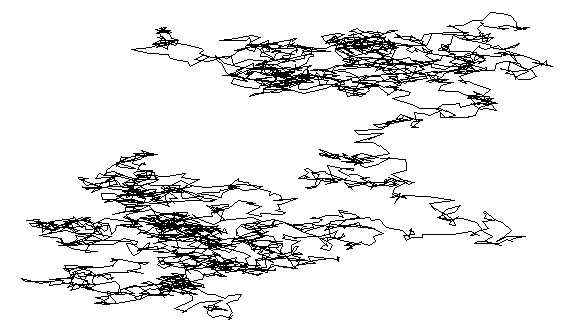
\includegraphics[height=0.05\textheight]{BM2d(1).png}
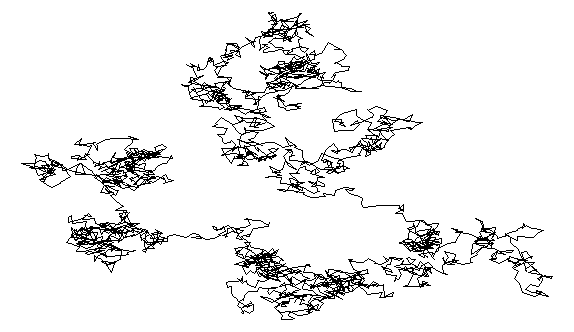
\includegraphics[height=0.05\textheight]{BM2d(2).png}
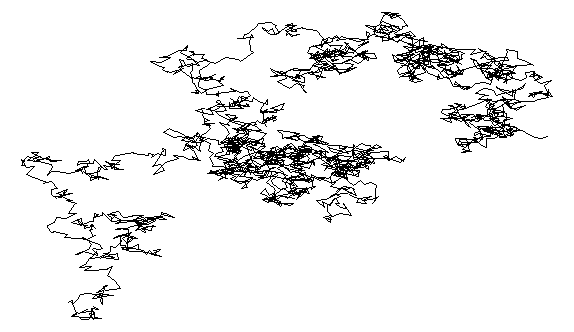
\includegraphics[height=0.05\textheight]{BM2d(3).png}
\end{Eg}

\begin{Eg}[Brown运动首中时]
设$(B_{t})_{t \ge 0}$是零初值标准Brown运动, $T_{b} := \inf\{ t \ge 0 : B_{t} = b \}$, $b \in \R$. 熟知$\P\{ T_{b} \in \d t \} = \frac{\abs{b}}{\sqrt{2\pi t^3}} \e^{-\frac{b^2}{2t}} \d t$和$\E\,\e^{-aT_b} = \e^{-\abs{b}\sqrt{2a}}$, $a \ge 0$. 下面考虑
\[ T_{b}^{(\mu)} := \inf\{ t \ge 0 : B_{t} + \mu t = b \} , \]
其中$\mu \in \R$是\emph{漂移}系数. 定义概率$\tilde{\P}$适合$\d\tilde{\P}/\d\P \,\big|_{\mathscr{F}_{t}} = Z_{t} := \e^{\mu B_{t} - \frac{1}{2}\mu^{2}t}$, $\forall t \ge 0$, 则$(B_{t} - \mu t)_{t \ge 0}$是零初值$\tilde{\P}$-标准Brown运动. 故
\[ \P\{ T_{b}^{(\mu)} \le t \} = \tilde{\P}\{ T_{b} \le t \} 
= \E\big[ Z_{t} \1_{\{ T_{b} \le t \}} \big] 
= \E\big[ Z_{T_{b}} \1_{\{ T_{b} \le t \}} \big] 
= \e^{\mu b} \, \E\big[ \e^{-\frac{1}{2}\mu^{2}T_{b}} \1_{\{ T_{b} \le t \}} \big] , \]
进而有$\P\{ T_{b}^{(\mu)} < \infty \} = \e^{\mu b - \abs{\mu b}}$和$\P\{ T_{b}^{(\mu)} \in \d t \} = \e^{\mu b - \frac{1}{2}\mu^{2}t} \, \P\{ T_{b} \in \d t \} = \frac{\abs{b}}{\sqrt{2\pi t^3}} \e^{-\frac{(b -\mu t)^2}{2t}} \d t$.
\end{Eg}


\begin{Thm}\label{Thm:expMG}
设$M = (M_{t})_{t \in [0,T]} \in \mathcal{M}_{\mathrm{cts},\mathrm{loc}}$, 其中$T \in [0,\infty]$固定, 则下述条件满足$\eqref{Condition:Novikov}\Rightarrow\eqref{Condition:Kazamaki}\Rightarrow\eqref{Condition:expMG}$.
\begin{enumerate}[\quad\normalfont (1)]
	\setlength{\itemsep}{0ex}
\item\label{Condition:Novikov} $\E\,\e^{\frac{1}{2}\agp{M}_{T}} < \infty$. \ {\normalfont (Novikov)}
\item\label{Condition:Kazamaki} $\sup_{\text{停时}\,\tau \le T} \E\,\e^{\frac{1}{2}M_{\tau}} < \infty$, 从而$M \in \mathcal{M}^{2}$. \ {\normalfont (Kazamaki)}
\item\label{Condition:expMG} $\mathcal{E}(M) = (\e^{M_{t}-\frac{1}{2}\agp{M}_{t}})_{t \in [0,T]}$是(一致可积)鞅.
\end{enumerate}
\end{Thm}


\begin{Ex}[\cite{Karatzas-Shreve--GTM113}~\S3.5; \cite{龚光鲁-钱敏平}~\S1.10]
阅读.
\end{Ex}


\begin{Ex}[\cite{龚光鲁-钱敏平}~引理~1.9]
证明: 适应于滤流$(\mathscr{F}_{t})_{t \ge 0}$的上鞅$(X_{t})_{t \ge 0}$是鞅当且仅当$\E X_{t}$不依赖$t$.
\begin{Prf}
随机变量$\as$不等式取等当且仅当两端期望相等.
\end{Prf}
\end{Ex}


\begin{Ex}[\cite{Karatzas-Shreve--GTM113}~3.5.18, \cite{Revuz-Yor}~VIII.1.24]
设$B = (B_{t})_{t \in [0,1]}$是零初值标准Brown运动, 定义停时$\tau := \inf\{ t : t + B_{t}^{2} = 1 \}$和随机过程$X = (X_{t})_{t \in [0,1)}$, 其中$X_{t} := -2(1-t)^{-2}B_{t}\1_{\{t\le\tau\}}$.
\begin{enumerate}
	\setlength{\itemsep}{0ex}
\item 证明$\as$有$\tau < 1$, 从而$\int_{0}^{1} X_{t}^{2} \d t < \infty$.
\begin{Prf}
由轨道连续性易见$\tau \le 1$, 且\[ \P\{ \tau = 1 \} \le \P\{ \max_{t \le 1-\delta} (t+B_{t}^{2}) < 1 \} \le \P\{ B_{1-\delta}^{2} < \delta \} \xrightarrow[\delta \searrow 0]{} 0 . \]
而$X_{t}^{2} = 4(1-t)^{-4}B_{t}^{2}\1_{\{t\le\tau\}} \le 4(1-t)^{-3}\1_{\{t\le\tau\}}$, 所以$\int_{0}^{1} X_{t}^{2} \d t \le 4 \int_{0}^{\tau} (1-t)^{-3} \d t < \infty ~\as$.
\end{Prf}
\item 对$((1-t)^{-2}B_{t}^{2})_{t \in [0,1)}$应用It\^{o}公式, 得出\[ \tint_{0}^{1} X \d B - \frac{1}{2}\int_{0}^{1} X_{t}^{2} \d t = -1 -2 \int_{0}^{\tau} [(1-t)^{-4}-(1-t)^{-3}] B_{t}^{2} \d t \le -1 . \vspace{-4.5ex}\]
\begin{Prf}
直接计算, $\d ((1-t)^{-2}B_{t}^{2}) = (2(1-t)^{-3}B_{t}^{2} + (1-t)^{-2}) \d t + 2(1-t)^{-2}B_{t} \d B_{t}$, 从而
\[\begin{aligned}
\tint_{0}^{1} X \d B = -2 \tint_{t=0}^{\tau} (1-t)^{-2}B_{t} \d B_{t} 
&= \tint_{0}^{\tau} (2(1-t)^{-3}B_{t}^{2} + (1-t)^{-2}) \d t - (1-\tau)^{-2}B_{\tau}^{2} \\
&= 2 \tint_{0}^{\tau} (1-t)^{-3}B_{t}^{2} \d t + [\bcancel{(1-\tau)^{-1}}-1] - \cancel{(1-\tau)^{-2}(1-\tau)} .
\end{aligned}\]
结合$\frac{1}{2}\int_{0}^{1} X_{t}^{2} \d t = 2 \int_{0}^{\tau} (1-t)^{-4}B_{t}^{2} \d t$即得所求.
\end{Prf}
\item 证明指数上鞅$Z := \mathcal{E}(\int X \d B) = (\e^{\int_{0}^{t} X \d B - \frac{1}{2}\int_{0}^{t} X_{s}^{2} \d s})_{t \in [0,1]}$不是鞅, 而$Z^{\sigma_{n}} = (Z_{t\wedge\sigma_{n}})_{t \in [0,1]}$是鞅, 其中$\sigma_{n} := 1-\frac{1}{\sqrt{n}}$, $n \in \{1,2,3,\cdots\}$.
\begin{Prf}
由于$Z_{1} \le \e^{-1} < 1 = Z_{0}$, 可见$Z$不是鞅. 记$M := \int X \d B$, 则$Z^{\sigma_{n}} = \mathcal{E}(M^{\sigma_{n}})$. 因为
\[ \agp{M^{\sigma_{n}}}_{1} = \agp{M}_{\sigma_{n}} = \tint_{0}^{\sigma_{n}} X_{t}^{2} \d t \le 4 \int_{0}^{\sigma_{n}} (1-t)^{-3} \d t = 2[(1-\sigma_{n})^{-2}-1] = 2n-2 < \infty , \]
可见Novikov条件成立, 故$Z^{\sigma_{n}}$是鞅.
\end{Prf}
\end{enumerate}
\end{Ex}


\begin{Ex}[\cite{Revuz-Yor}~VIII.1.23]
设$B = (B_{t})_{t \ge 0}$是零初值标准Brown运动, $\tau$是满足$\E\,\e^{\frac{1}{2}\tau} < \infty$的停时. 证明$\E\,\e^{B_{\tau}-\frac{1}{2}\tau} = 1$.
\begin{Prf}
停止Brown运动$B^{\tau} = (B_{t\wedge\tau})_{t \in [0,\infty]}$的特征为$\agp{B^{\tau}} = (t\wedge\tau)_{t \in [0,\infty]}$, 依题意满足Novikov条件. 由此立得$\mathcal{E}(B^{\tau}) = (\e^{B_{t\wedge\tau}-\frac{1}{2}(t\wedge\tau)})_{t \in [0,\infty]}$是一致可积鞅, 从而$\E\,\e^{B_{\tau}-\frac{1}{2}\tau} = \E\,\mathcal{E}(B^{\tau})_{\infty} = 1$.
\end{Prf} 
\end{Ex}


\begin{Ex}[\cite{Revuz-Yor}~VIII.1.36]
考虑样本空间$\Omega := C([0,1];\R)$, 配备Wiener测度$\P$和自然滤流$(\mathscr{F}_{t})_{t \in [0,1]}$. 取定有界可料过程$b = (b_{t})_{t \in [0,1]}$. 对于$\omega\in\Omega$, 置$\d\tilde{\P}(\omega) := \e^{\int_{0}^{1} b_{t}(\omega) \d\omega(t) - \frac{1}{2}\int_{0}^{1} b_{t}(\omega)^{2} \d t} \d\P(\omega)$和
\[ \theta(\omega) : t \in [0,1] \mapsto \omega(t) - \tint_{0}^{t} b_{s}(\omega) \d s \in \R . \]
证明: 若$(M_{t})_{t \in [0,1]}$是$\P$-(局部)鞅, 则$(M_{t}\circ\theta)_{t \in [0,1]}$是$\tilde{\P}$-(局部)鞅. \\
例如, 若$u \in C^{1,2}([0,1]\times\R;\R)$满足$\p{u}{t} + \frac{1}{2}\p[2]{u}{x} = 0$, 则$\big( u(t,\theta(\bm{\cdot})(t)) \big)_{t \in [0,1]}$是$\tilde{\P}$-(局部)鞅.
\begin{Prf}
利用局部鞅表示定理(\cite{Revuz-Yor}~V.3.4), 存在常数$C$和局部平方可积可料过程$(H_{s})_{s \in [0,1]}$, 使得
\[ M_{t}(\omega) = C + \tint_{0}^{t} H_{s}(\omega) \d\omega(s) . \]
由于$\theta$是可测双射, $(H_{s}\circ\theta)_{s \in [0,1]}$仍是局部平方可积可料过程. 
根据Girsanov定理, $\big(\theta(\bm{\cdot})(t)\big)_{t \in [0,1]}$是$\tilde{\P}$-Brown运动, 因此
\[ M_{t}\circ\theta(\omega) = C + \tint_{0}^{t} H_{s}\circ\theta(\omega) \d\theta(\omega)(s) \]
是$\tilde{\P}$-局部鞅. \textred{接下来只需说明可积性.} 易见$\tilde{\P}\theta^{-1} = \P$, 因而$\int \abs{M_{t}\circ\theta} \d\tilde{\P} = \int \abs{M_{t}} \d\P$.
\end{Prf}
\end{Ex}


\begin{Prop}[Wiener测度(平移)拟不变性]
考虑样本空间$\Omega := C([0,T];\R)$, 配备Borel代数$\mathscr{B}$和Wiener测度$\P$, 从而有零初值标准Brown运动$W : (t,w) \in [0,T]\times\Omega \mapsto W_{t}(w) := w(t) \in \R$. 令
\[ W^{(\varepsilon h)} : (t,w) \in [0,T]\times\Omega \mapsto W^{(\varepsilon h)}_{t}(w) := w(t) - \varepsilon \tint_{0}^{t} h(s) \d s \in \R , \]
其中$h \in L^{2}([0,T])$, $\varepsilon \in (-1,1)$, 则对$A \in \mathscr{B}$有$\P\{ W \in A \} = 0 \iff \P\{ W^{(\varepsilon h)} \in A \} = 0$.
\begin{proof}
利用定理\ref{Thm:Cameron--Martin}可得与$\P$相互绝对连续的$\tilde{\P}^{\varepsilon}$, 使$W^{(\varepsilon h)}$成为零初值$\tilde{\P}^{\varepsilon}$-标准Brown运动.
\end{proof}
特别地, 对于$\Omega$上的可测函数$F$和$G$, 如果$F(W) \stackrel{\as}{=} G(W)$, 那么$F(W^{(\varepsilon h)}) \stackrel{\as}{=} G(W^{(\varepsilon h)})$.
\end{Prop}
\begin{Prop}[Malliavin导数]
$\mathrm{D}_{h}F(W) := \p{}{\varepsilon}\big|_{\varepsilon=0} F(W^{(-\varepsilon h)})$满足$\E\big[\mathrm{D}_{h}F(W)\big] = \E\big[ F(W) \int_{t=0}^{T} h(t) \d W_{t} \big]$.
\begin{proof}
在$\P$下, $F(W^{(-\varepsilon h)}) - F(W) \stackrel{d}{=} F(W) (\frac{\d\tilde{\P}^{\varepsilon}}{\d\P} - 1)$, 且$\p{}{\varepsilon}\big|_{\varepsilon=0} \frac{\d\tilde{\P}^{\varepsilon}}{\d\P} = \int_{t=0}^{T} h(t) \d W_{t}$.
\end{proof}
\normalfont 更多内容可参看M.~Hairer. (2021+). \href{http://www.hairer.org/notes/Malliavin.pdf}{Introduction to Malliavin Calculus}.
\end{Prop}



\section{局部时·动机 \normalfont\footnotesize (2021年11月22日)}
\begin{Eg}
在例\ref{Eg:BM_approximate_function}中, $\d\tilde{\P}/\d\P = \e^{\int_{t=0}^{T} f'(t) \d B_{t} - \frac{1}{2} \int_{0}^{T} f'(t)^{2} \d t}$. 我们有
\[ \frac{\P\{ \max_{t \in [0,T]} \abs{B_{t}-f(t)} < \varepsilon \}}{\P\{ \max_{t \in [0,T]} \abs{B_{t}} < \varepsilon \}} = \frac{\P\{ \max_{t \in [0,T]} \abs{\tilde{B}_{t}} < \varepsilon \}}{\tilde{\P}\{ \max_{t \in [0,T]} \abs{\tilde{B}_{t}} < \varepsilon \}} \xrightarrow[\varepsilon \searrow 0]{} \frac{\d\P}{\d\tilde{\P}}\bigg|_{\{\tilde{B} \equiv 0\}} = \e^{- \frac{1}{2} \int_{0}^{T} f'(t)^{2} \d t} . \]
\end{Eg}
\begin{Eg}
设$B = (B_{t})_{t \ge 0}$是($n$维)标准Brown运动. 若$B_{0} = 0$, 则$B \stackrel{d}{=} (\varepsilon B_{t/\varepsilon^2})_{t \ge 0}$, $\forall \varepsilon > 0$. 于是
\[ \P( \max_{t \in [0,T]} \abs{B_{t}} < \varepsilon \,|\, B_{0}=0 ) = \P( \max_{t \in [0,T/\varepsilon^{2}]} \abs{B_{t}} < 1 \,|\, B_{0}=0 ) = \P( \sigma > T/\varepsilon^{2} \,|\, B_{0}=0 ) , \] 其中$\sigma := \inf\{ t : \abs{B_{t}} \ge 1 \}$. 
令$u(t,x) := \E[ f(B_{t}) \1_{\{\sigma>t\}} \,|\, B_{0}=x ]$, 其中$f$定义于$\{ x \in \R^{n} : \abs{x} < 1 \}$. \clearpage\noindent
可得\[\begin{cases}
\p{u}{t} = \frac{1}{2} \Delta_{x} u , \ t \ge 0 ,\, \abs{x} < 1 , \\
u|_{t=0} = f , \ u|_{\abs{x}=1} = 0 .
\end{cases}\]
设$\phi_{n}$是$-\frac{1}{2}\Delta$的特征函数: \[\begin{cases}
\frac{1}{2}\Delta_{x}\phi_{n} + \lambda_{n}\phi_{n} = 0 , \ \abs{x}<1 , \\
\qquad\quad\phi_{n}|_{\abs{x}=1} = 0 . 
\end{cases}\]
则有$u(t,x) = \sum_{n=1}^{\infty} \e^{-\lambda_{n}t} \phi_{n}(x) \int_{\abs{y}<1} \phi_{n}(y) f(y) \d y$, 其中$0 < \lambda_{1} < \lambda_{2} < \dots$. 特别地, 当$\varepsilon \searrow 0$时, \[ \P( \sigma > T/\varepsilon^{2} \,|\, B_{0}=0 ) = \tsum_{n=1}^{\infty} \e^{-\lambda_{n}T/\varepsilon^{2}} \phi_{n}(0) \int_{\abs{y}<1} \phi_{n}(y) \d y \sim \e^{-\lambda_{1}T/\varepsilon^{2}} \phi_{1}(0) \int_{\abs{y}<1} \phi_{1}(y) \d y . \]
\normalfont\small\Pickup 参看N.~Ikeda; S.~Watanabe. (1989). \emph{Stochastic Differential Equations and Diffusion Processes} (2nd ed.). \S6.9.
\end{Eg}

\begin{Eg}[Brown局部时]
对于一维标准Brown运动$B = (B_{t})_{t \ge 0}$, L\'{e}vy证明了$\as$存在有限的
\[ L^{a}_{t}(B) := \lim_{\varepsilon \searrow 0} \frac{1}{2\varepsilon} \int_{0}^{t} \1_{\{ \abs{B_{s}-a} < \varepsilon \}} \d s , \quad t \ge 0 ,\ a \in \R . \]
形式上, $L^{a}_{t}(B) = \int_{0}^{t} \delta_{a}(B_{s}) \d s$, 从而适用于非光滑分析.
\end{Eg}


\begin{Ex}[\cite{龚光鲁-钱敏平}~\S4.5]
阅读.
\end{Ex}


\begin{Ex}\label{Ex:Ito_C1}
设$g \in C^{1}(\R;\R)$在有限个点外二阶连续可微, $g''$在不连续处左右极限存在, 并且$g''$有界. 对于一维标准Brown运动$(B_{t})_{t \ge 0}$, 证明$g(B_{t}) = g(B_{0}) + \int_{0}^{t} g'(B) \d B + \frac{1}{2}\int_{0}^{t} g''(B_{s}) \d s$.
\begin{Prf}
用磨光子$j_{\varepsilon} := \frac{1}{\varepsilon}j(\frac{\bm{\cdot}}{\varepsilon})$与$g$作卷积得到光滑函数$g * j_{\varepsilon}$, 应用It\^{o}公式然后令$\varepsilon \searrow 0$.
\end{Prf}
\end{Ex}



\section{局部时·Tanaka公式 \normalfont\footnotesize (2021年11月24日)}
\begin{Eg}
设$B = (B_{t})_{t \ge 0}$是一维标准Brown运动, 则
\[ \abs{B_{t}-a} = \abs{B_{0}-a} + \tint_{0}^{t} \sgn{B-a} \d B + L_{t}^{a}(B) ,\quad  t \ge 0 ,\ a \in \R . \]
\begin{proof}
对$g_{\varepsilon}(B) = \abs{B-a}\1_{\{\abs{B-a}\ge\varepsilon\}} + (\frac{(B-a)^2}{2\varepsilon}+\frac{\varepsilon}{2})\1_{\{\abs{B-a}<\varepsilon\}}$应用习题\ref{Ex:Ito_C1}, 然后令$\varepsilon \searrow 0$.
\end{proof}
\noindent 类似地, $\begin{cases}
(B_{t}-a)^{+} = (B_{0}-a)^{+} + \tint_{0}^{t} \1_{(a,\infty)}(B) \d B + \frac{1}{2} L_{t}^{a}(B) , \\
(B_{t}-a)^{-} = (B_{0}-a)^{-} - \tint_{0}^{t} \1_{(-\infty,a]}(B) \d B + \frac{1}{2} L_{t}^{a}(B) . 
\end{cases}$
\end{Eg}

\begin{Thm}[Tanaka]\label{Thm:Tanaka}
设$X = (X_{t})_{t \ge 0}$是一维连续半鞅, $a \in \R$, 则存在增过程$L^{a}(X) = (L_{t}^{a}(X))_{t \ge 0}$, 使得对任意$t \ge 0$成立$\begin{cases}
(X_{t}-a)^{+} = (X_{0}-a)^{+} + \tint_{0}^{t} \1_{(a,\infty)}(X) \d X + \frac{1}{2} L_{t}^{a}(X) , \\
(X_{t}-a)^{-} = (X_{0}-a)^{-} - \tint_{0}^{t} \1_{(-\infty,a]}(X) \d X + \frac{1}{2} L_{t}^{a}(X) , \\
\abs{X_{t}-a} = \abs{X_{0}-a} + \tint_{0}^{t} \sgn{X-a} \d X + L_{t}^{a}(X) . 
\end{cases}$
\begin{Def}[局部时]
定理\ref{Thm:Tanaka}中$L^{a}(X)$称为$X$在水平$a$处的\textbf{局部时}, 且
\begin{Rmk}
$(t,\omega,a) \mapsto L_{t}^{a}(X)(\omega)$是$(\mathscr{P}\otimes\mathscr{B}_{\R})/\mathscr{B}_{[0,\infty)}$可测的; 特别地, $L^{a}(X)$可料, $\forall a \in \R$.
\end{Rmk}
\end{Def}
\end{Thm}

\begin{Prop}
连续半鞅$X$的局部时$t \mapsto L_{t}^{a}(X)$生成的Lebesgue--Stieltjes测度支撑于$\{ t : X_{t} = a \}$.
\begin{proof}
对$(X-a)^{2} = \abs{X-a}^{2}$两端分别应用It\^{o}公式, 可得$\int_{t=0}^{T} \abs{X_{t}-a} \d L^{a}_{t}(X) = 0$, $\forall T > 0$.
\end{proof}
\end{Prop}

\begin{Thm}[It\^{o}--Tanaka--Meyer]
设$X = (X_{t})_{t \ge 0}$是连续半鞅, $f$是凸函数, $f'_{-}$是$f$的左导数, 则
\[ f(X_{t}) = f(X_{0}) + \int_{0}^{t} f'_{-}(X) \d X + \frac{1}{2}\int_{\R} L_{t}^{a}(X) \d f'_{-}(a) , \quad t \ge 0 . \]
\end{Thm}

\begin{Prop}
若$X = (X_{t})_{t \ge 0}$是连续半鞅, 则$L_{t}^{a}(X)$关于$t$连续且关于$a$右连左极. \par
进一步地, 若$M = (M_{t})_{t \ge 0}$是连续鞅, 则$L_{t}^{a}(M)$关于$t$和$a$均连续.
\end{Prop}

\begin{Thm}[占位时]
设$X = (X_{t})_{t \ge 0}$是连续半鞅, $g : \R \to \R$是有界可测函数, 则
\[ \tint_{s=0}^{t} g(X_{s}) \d\agp{X}_{s} = \tint_{\R} g(a) L_{t}^{a}(X) \d a ,\quad \forall t \ge 0 . \]
\end{Thm}
\begin{Cor}
连续半鞅$X = (X_{t})_{t \ge 0}$的局部时满足$L_{t}^{a}(X) = \lim_{\varepsilon \searrow 0} \frac{1}{\varepsilon} \int_{s=0}^{t} \1_{[a,a+\varepsilon)}(X_{s}) \d\agp{X}_{s}$. \par
进一步地, 连续鞅$M = (M_{t})_{t \ge 0}$的局部时满足$L_{t}^{a}(M) = \lim_{\varepsilon \searrow 0} \frac{1}{2\varepsilon} \int_{s=0}^{t} \1_{(a-\varepsilon,a+\varepsilon)}(M_{s}) \d\agp{M}_{s}$.
\end{Cor}


\begin{Ex}[\cite{龚光鲁-钱敏平}:~\S2.8,~\S2.9; \cite{Karatzas-Shreve--GTM113}:~\S3.6,~\S3.7]
阅读. 注意\cite{Karatzas-Shreve--GTM113}中的局部时额外乘了系数$\frac{1}{2}$.
\end{Ex}


\begin{Ex}[\cite{龚光鲁-钱敏平}~引理2.26; \cite{Karatzas-Shreve--GTM113}:~3.6.12,~3.7.7]
阅读证明\textbf{Fubini型定理}:\par 设$M = (M_{t})_{t \ge 0} \in \mathcal{M}_{\mathrm{loc}}^{2}$, $\mu$是$(\R,\mathscr{B}_{\R})$上$\sigma$-有限测度, $(\Phi_{t}^{x})^{x \in \R}_{t \ge 0}$是随机场, 且$(t,\omega,x) \mapsto \Phi_{t}^{x}(\omega)$是$(\mathscr{P}\otimes\mathscr{B}_{\R})/\mathscr{B}_{\R}$可测的. 若存在$f \in L^{1}(\mu)$使得$\forall x \in \R$都有$\sup_{t,\omega}\abs{\Phi_{t}^{x}(\omega)} \le f(x)$, 且$\forall T \ge 0$都有$(\omega,x) \mapsto \int_{t=0}^{T} \Phi_{t}^{x} \d M_{t}$可测, 则$\big( \int_{\R} \Phi_{t}^{x} \d\mu(x) \big)_{t \ge 0} \in \mathcal{L}^{*}_{\mathrm{loc}}(M)$, 且
\[ \int_{t=0}^{T}\bigg( \int_{\R} \Phi_{t}^{x} \d\mu(x) \bigg)\d M_{t} = \int_{\R}\bigg( \int_{t=0}^{T} \Phi_{t}^{x} \d M_{t} \bigg)\d\mu(x) ,\quad T \ge 0 . \]
\end{Ex}


\begin{Ex}
证明连续有限变差过程$X = (X_{t})_{t \ge 0}$的局部时恒为零.
\begin{Prf}
$\int_{0}^{t} \sgn{X-a} \d X = \int_{s=0}^{t} \sgn{X_{s}-a} \d X_{s} = \int_{s=0}^{t} \d\abs{X_{s}-a} = \abs{X_{t}-a} - \abs{X_{0}-a}$, $\forall a \in \R$.
\end{Prf}
\end{Ex}



\subsection*{局部时·应用 \normalfont\footnotesize (2021年12月1日)}
\begin{Lem}[Skorokhod]
设$y : [0,\infty) \to \R$连续, $y(0) \ge 0$, 则存在唯一的$x : [0,\infty) \to [0,\infty)$和$a : [0,\infty) \to [0,\infty)$, 使得$x = y+a$, 且$a$零初值、连续、递增、生成的Lebesgue--Stieltjes测度支撑于$\{ t : x(t) = 0 \}$. 事实上, $a(t) = 0 \vee \max_{s \in [0,t]} \{-y(s)\}$.
\vspace{-3ex}\par\hfill\color{gray}Credit:~\textsc{Y.-F.~Chen}~~~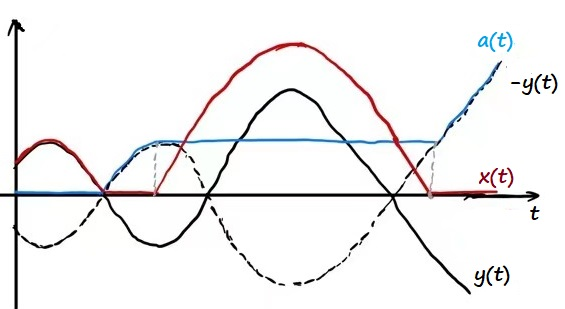
\includegraphics[height=0.1\textheight]{Skorokhod.jpg}
\end{Lem}
\begin{Cor}
设$B$是零初值一维标准Brown运动, 则$L^{0}_{t}(B) = \max_{s \in [0,t]} \beta_{s}$, 其中$\beta := - \int \sgn{B} \d B$也是零初值一维标准Brown运动(例\ref{Eg:sgn_BM}).
\end{Cor}
\begin{Thm}[L\'{e}vy]
设$B = (B_{t})_{t \ge 0}$是零初值一维标准Brown运动, $M_{t} := \max_{s \in [0,t]} B_{s}$, 则
\[ (M_{t}-B_{t},M_{t})_{t \ge 0} \stackrel{d}{=} (\abs{B_{t}},L^{0}_{t}(B))_{t \ge 0} . \]
\end{Thm}




\section{随机微分方程 \normalfont\footnotesize (2021年12月1日)}
设$B = (B_{t})_{t \ge 0}$是($n$维)标准Brown运动, 考虑($m$维)扩散过程$X = (X_{t})_{t \ge 0}$满足
\[ \d X_{t} = b(t,X_{t}) \d t + \sigma(t,X_{t}) \d B_{t} , \label{eq:SDE}\tag{SDE}\]
其中称$b = (b^{i})^{1\le i\le m} : [0,\infty)\times\R^{m} \to \R^{m}$为\textbf{漂移系数}, $\sigma = (\sigma^{i}_{j})^{1\le i\le m}_{1\le j\le n} : [0,\infty)\times\R^{m} \to \R^{m\times n}$为\textbf{弥散系数}.
定义$a = (a^{ik})^{1 \le i,k \le m} := \sigma\sigma^{\top} = (\sum_{j=1}^{n} \sigma^{i}_{j}\sigma^{k}_{j})^{1 \le i,k \le m} : [0,\infty)\times\R^{m} \to \R^{m\times m}$, 称为\textbf{扩散系数}.

\begin{Def}[强解]
连续适应随机过程$X = (X_{t})_{t \ge 0}$称为\eqref{eq:SDE}的\textbf{强解}, 若
\begin{itemize}
	\item $(b(t,X_{t}))_{t \ge 0} \in \mathcal{L}^{1}_{\mathrm{loc}}([0,\infty)) := \{ \text{适应}\,(Z_{t})_{t \ge 0} : (t \mapsto Z_{t}) \in L^{1}_{\mathrm{loc}}([0,\infty)) ~\as \}$, 
	\item $(\sigma(t,X_{t}))_{t \ge 0} \in \mathcal{L}_{\mathrm{loc}}^{*}(B) = \{ \text{循序可测}\,(Z_{t})_{t \ge 0} : (t \mapsto Z_{t}) \in L^{2}_{\mathrm{loc}}([0,\infty)) ~\as \}$, 且
	\item $X_{t} = X_{0} + \int_{0}^{t} b(s,X_{s}) \d s + \int_{s=0}^{t} \sigma(s,X_{s}) \d B_{s}$, $t \ge 0$.
\end{itemize}
\end{Def}
\begin{Def}[轨道(强)唯一性]
关于\eqref{eq:SDE}的\textbf{强唯一性}成立, 若初值给定的任意两个强解不可区分.
\end{Def}

\begin{Eg}
一维\ref{eq:SDE}~$\d X_{t} = b(t,X_{t}) \d t + \d B_{t}$有强唯一性, 若$b$有界且$\forall t \ge 0$都有$b(t,\bm{\cdot})$递减.
\end{Eg}

\begin{Thm}
考虑\eqref{eq:SDE}. 若$b$和$\sigma$满足
\begin{itemize}
	\item (全局Lipschitz条件) $\abs{b(t,x)-b(t,y)}+\abs{\sigma(t,x)-\sigma(t,y)} \lesssim \abs{x-y}$, 和
	\item (线性增长条件) $\abs{b(t,x)}+\abs{\sigma(t,x)} \lesssim \abs{x} + 1$, 
\end{itemize}
则任给$\xi \in L^{2}(\mathscr{F}_{0})$, 存在强解$X = (X_{t})_{t \ge 0}$使之初值为$X_{0} = \xi$. 任取$T \in [0,\infty)$, 有
\[ \log \norm{X_{t}}_{L^{2}(\P)} \lesssim_{L(b,\sigma),T} t + 1 + \log(1+\norm{\xi}_{L^{2}(\P)}) ,\quad t \in [0,T] , \]
其中$L(b,\sigma)$表示$(b,\sigma)$的Lipschitz常数和线性增长率.
\begin{proof}
用Picard迭代构造解, 用Gronwall不等式给出二阶矩的估计.
\end{proof}
\end{Thm}


\begin{Ex}[\cite{Karatzas-Shreve--GTM113}:~\S5.1,~\S5.2; \cite{龚光鲁-钱敏平}~\S3.1]
阅读; 注意强解存在性证明中的局部化技巧.
\end{Ex}


\begin{Ex}
利用Picard迭代求解线性随机微分方程$\d X_{t} = \lambda X_{t} \d B_{t}$, 其中$B = (B_{t})_{t \ge 0}$是零初值一维标准Brown运动, $X_{0} = \xi$与$B$独立, $\lambda$是常数.
\begin{Soln}
归纳定义$X^{(n)} := \xi + \lambda \int X^{(n-1)} \d B$, 其中$X^{(0)} \equiv \xi$. 由命题\ref{Prop:Hermite_polynomial_differential}可得$X^{(n)}_{t} = \xi \sum_{k=0}^{n} \frac{\lambda^k}{k!} H_{k}(B_{t},t)$, 于是$X = \lim_{n\to\infty}X^{(n)} = \xi \, \mathcal{E}(\lambda B)$.
\end{Soln}
\end{Ex}


\begin{Ex}
在爆炸时之前, 求解$\d X_{t} = \frac{1}{2}\e^{-2X_{t}} \d t + \e^{-X_{t}} \d X_{t}$, $X_{0} = a \in \R$.
\begin{Soln}
整理可得$\d t = 2 (\e^{2X_{t}}-\e^{X_{t}}) \d X_{t} = \d(\e^{2X_{t}}-2\,\e^{X_{t}})$, 则$\e^{2X_{t}}-2\,\e^{X_{t}} = t+\e^{2a}-2\,\e^{a}$, 进而解得$X_{t} = \log\big(1+\eps_{a}\sqrt{t+(\e^{a}-1)^{2}}\big)$, $0 \le t < (2\,\e^{a}-\e^{2a})\vee(\eps_{a}\infty)$, 其中$\eps_{a} := \sgn{a}\1_{[a \neq 0]} \pm \1_{[a = 0]}$.
\end{Soln}
\end{Ex}


\begin{Ex}[\cite{Karatzas-Shreve--GTM113}~5.2.17]
设$B = (B_{t})_{t \ge 0}$是一维标准Brown运动. 证明$\d X_{t} = 3 X_{t}^{1/3} \d t + 3 X_{t}^{2/3} \d B_{t}$有不可数个强解形如$X_{t}^{(\theta)} := B_{t}^{3} \1_{\{t\ge\tau_{\theta}\}}$, 其中$\tau_{\theta} := \inf\{ t \ge \theta : B_{t} = 0 \}$, $\theta \in [0,\infty]$.
\begin{Prf}
对$X_{t}^{(\theta)} = (B_{t}\1_{\{t\ge\tau_{\theta}\}})^{3}$应用It\^{o}公式, 有\par\hspace{-1em}
$\d X_{t}^{(\theta)} = 3(B_{t}\1_{\{t\ge\tau_{\theta}\}})^{2}\d(B_{t}\1_{\{t\ge\tau_{\theta}\}}) + 3(B_{t}\1_{\{t\ge\tau_{\theta}\}})\d(t\1_{\{t\ge\tau_{\theta}\}}) = 3 (X_{t}^{(\theta)})^{2/3} \d B_{t} + 3 (X_{t}^{(\theta)})^{1/3} \d t$.
\end{Prf}
\end{Ex}



\section{随机微分方程·续 \normalfont\footnotesize (2021年12月6日+8日)}
\begin{Prop}[Yamada--Watanabe]
一维\ref{eq:SDE}的解具有强唯一性, 若成立Osgood条件:
\[ \abs{b(t,x)-b(t,y)} \le k(\abs{x-y}) , \quad\&\quad \abs{\sigma(t,x)-\sigma(t,y)} \le h(\abs{x-y}) , \]
其中$k,h : [0,\infty) \to [0,\infty)$是零初值严格递增函数, $k$凹, 且$\int_{0}^{\eps} \frac{\d u}{k(u)} = \int_{0}^{\eps} \frac{\d u}{h(u)^{2}} = \infty$, $\forall \eps > 0$.
\end{Prop}\clearpage

\begin{Prop}[比较定理]\label{Prop:comparison}
设$B = (B_{t})_{t \ge 0}$是一维标准Brown运动, $X^{i} = (X^{i}_{t})_{t \ge 0}$是一维随机微分方程$\d X^{i}_{t} = b_{i}(t,X^{i}_{t}) \d t + \sigma(t,X^{i}_{t}) \d B_{t}$的唯一存在的强解, $i = 1,2$. 若$b_{1} \le b_{2}$且其一满足Lipschitz条件, $X^{1}_{0} \le X^{2}_{0}$, 则$\P\{ X^{1}_{t} \le X^{2}_{t} ,\ \forall t \ge 0 \} = 1$.
\begin{proof}
由占位时公式, 可得$L^{0}(X^{1}-X^{2}) = 0$. 接下来对$(X^{1}-X^{2})^{+}$应用It\^{o}--Tanaka公式, 取期望后代入Lipschitz条件, 从而可以利用Gronwall不等式.
\end{proof}
\end{Prop}


\begin{Def}[弱解]
随机过程$\tilde{X} = (\tilde{X}_{t})_{t \ge 0}$称为\eqref{eq:SDE}的\textbf{弱解}, 若$\tilde{X}$是某个(新的)带滤流概率空间上的随机微分方程$\d\tilde{X}_{t} = b(t,\tilde{X}_{t}) \d t + \sigma(t,\tilde{X}_{t}) \d\tilde{B}_{t}$的强解, 其中$\tilde{B} = (\tilde{B}_{t})_{t \ge 0}$是标准Brown运动.
\end{Def}
\begin{Def}[分布(弱)唯一性]
关于\eqref{eq:SDE}的\textbf{弱唯一性}成立, 若初分布给定的任意两个弱解同分布.
\end{Def}

\begin{Eg}[弱存在/唯一性\emph{不蕴涵}强存在/唯一性]
一维\ref{eq:SDE}~$\d X_{t} = \sgn{X_{t}} \d B_{t}$的弱解存在并且是标准Brown运动, 而$X$和$-X$必然同时为强解; 但是, 考虑$B$的自然滤流时, 强解不存在. 
\end{Eg}

\begin{Thm}
考虑\ref{eq:SDE}~$\d X_{t} = b(t,X_{t}) \d t + \d B_{t}$, $0 \le t \le T$, 其中$T$是固定正数, $b : [0,T]\times\R^{n} \to \R^{n}$满足线性增长条件$\abs{b(t,x)} \lesssim \abs{x} + 1$, 则对任意初分布都存在弱解. 如果(在各自的概率空间上)弱解$X^{i} = (X^{i}_{t})_{t \in [0,T]}$满足$\int_{0}^{T} \abs{b(t,X^{i}_{t})}^{2} \d t < \infty ~(\as)$, $i = 1,2$, 那么$X^{1} \stackrel{d}{=} X^{2}$.
\begin{proof}
应用Girsanov定理变换Brown运动: 原测度下的$X$, 新测度下的$(X_{t} - \int_{0}^{t} b(s,X_{s}) \d s)_{t \in [0,T]}$.
\end{proof}
\end{Thm}


\begin{Ex}[\cite{Karatzas-Shreve--GTM113}~5.2.19]
设$B = (B_{t})_{t \ge 0}$是一维标准Brown运动, $X^{i} = (X^{i}_{t})_{t \ge 0}$是一维随机微分方程$\d X^{i}_{t} = b_{i}(t,X^{i}_{t}) \d t + \sigma(t,X^{i}_{t}) \d B_{t}$的唯一存在的强解, 其中$b_{i} : [0,\infty)\times\R \to \R$连续, $i = 1,2$. 证明: 若$b_{1} < b_{2}$且$X^{1}_{0} \le X^{2}_{0}$, 则$\P\{ X^{1}_{t} \le X^{2}_{t} ,\ \forall t \ge 0 \} = 1$.
\begin{Prf}
取定$m > 233$, 则$b_{2}-b_{1}$在紧集$[0,m]\times[-m,m]$上的下界为正, 于是可构造Lipschitz连续的函数$b_{m} : [0,\infty)\times\R \to \R$使其在$[0,m]\times[-m,m]$上满足$b_{1} \le b_{m} \le b_{2}$. 设$X^{m} = (X^{m}_{t})_{t \ge 0}$是$\d X^{m}_{t} = b_{m}(t,X^{m}_{t}) \d t + \sigma(t,X^{m}_{t}) \d B_{t}$的初值为$X^{m}_{0}=X^{1}_{0}$的强解, 那么命题\ref{Prop:comparison}给出
\[ \P\big\{ X^{1}_{t} \le X^{m}_{t} \le X^{2}_{t} ,\ \forall t \le m \wedge \inf\{ t : \abs{X^{m}_{t}} > m \} \big\} = 1 . \]
令$m \to \infty$, 注意$m \wedge \inf\{ t : \abs{X^{m}_{t}} > m \} \ge m \wedge \inf\{ t : \abs{X^{1}_{t}}\vee\abs{X^{2}_{t}} > m \} \to \infty$, 即证所欲.
\end{Prf}
\end{Ex}


\begin{Ex}[\cite{Karatzas-Shreve--GTM113}~5.2.20]
考虑$\d X_{t} = b(X_{t}) \d t + \sigma(X_{t}) \d B_{t}$, 其中$B = (B_{t})_{t \ge 0}$是一维标准Brown运动, $b \in C^{1}(\R;\R)$, $\sigma \in C^{2}(\R;(0,\infty))$. 设$b'-\frac{1}{2}\sigma\sigma''-\frac{b\sigma'}{\sigma}$有界, 且$\frac{1}{\sigma}$在$\pm\infty$处均不可积. 给定初值后, 证明此方程存在唯一的强解.
\begin{Prf}
令$f := \int_{0}^{\bm{\cdot}} \frac{\d u}{\sigma(u)}$, 则有$f' = \frac{1}{\sigma} > 0$和$f'' = -\frac{\sigma'}{\sigma^2}$. 记$Y_{t} := f(X_{t})$, 则$X_{t} = f^{-1}(Y_{t})$. 由It\^{o}公式, $\d Y_{t} = f'(X_{t}) \d X_{t} + \frac{1}{2}f''(X_{t}) \d\agp{X}_{t} = \d B_{t} + ( \frac{b}{\sigma} - \frac{1}{2} \sigma' )(X_{t}) \d t = \d B_{t} + ( \frac{b}{\sigma} - \frac{1}{2} \sigma' )\circ f^{-1}(Y_{t}) \d t$, 这里将$Y$视作待求. 可见$\big( ( \frac{b}{\sigma} - \frac{1}{2} \sigma' )\circ f^{-1} \big)' = \big(( \frac{b'}{\sigma} - \frac{b\sigma'}{\sigma^2} - \frac{1}{2} \sigma'' )\frac{1}{f'} \big)\circ f^{-1} = ( b' - \frac{b\sigma'}{\sigma} - \frac{1}{2} \sigma\sigma'' )\circ f^{-1}$有界, 故$Y$的随机微分方程满足Lipschitz条件和线性增长条件. 强解$Y$存在唯一, 则$X$亦如是.
\end{Prf}
\end{Ex}


\begin{Ex}[\cite{Karatzas-Shreve--GTM113}~5.3.12]
考虑一维\ref{eq:SDE}~$\d X_{t} = -\sgn{X_{t}} \d t + \d B_{t} ,~ X_{0} = B_{0}$. 证明其弱解$X = (X_{t})_{t \ge 0}$满足$\P\{ X_{t} \in A \} = \e^{-t/2} \, \E[\1_{\{ B_{t} \in A \}} \, \e^{-\abs{B_{t}}+L_{t}^{0}(B)}]$, $A \in \mathscr{B}_{\R}$.
\begin{Prf}
由Tanaka公式, $-\abs{B_{t}}+L_{t}^{0}(B) = -\int_{0}^{t} \sgn{B} \d B$. 设概率测度$\tilde{\P}$满足$\frac{\d\tilde{\P}}{\d\P}\big|_{\mathscr{F}_{t}} = \e^{-t/2 -\int_{0}^{t} \sgn{B} \d B}$, 则$\tilde{B}_{t} := B_{t} + \int_{0}^{t} \sgn{B_{s}} \d s$在$\tilde{\P}$下是标准Brown运动. 我们有$\d B_{t} = -\sgn{B_{t}} \d t + \d\tilde{B}_{t}$, 于是$(B,\tilde{B})_{\#}\tilde{\P} = (X,B)_{\#}\P$. 特别地, $\P\{ X_{t} \in A \} = \tilde{\P}\{ B_{t} \in A \} = \E[\1_{\{ B_{t} \in A \}} \frac{\d\tilde{\P}}{\d\P}]$即为所求.
\end{Prf}
\end{Ex}


\begin{Ex}[\cite{Karatzas-Shreve--GTM113}:~\S5.3.A,~\S5.3.B]
阅读.
\end{Ex}



%\section{随机微分方程·再续 \normalfont\footnotesize (2021年12月8日)}
\begin{Prop}
考虑\eqref{eq:SDE}将$b$替换为$b + H \sigma$, 其中$H \in \mathcal{L}^{*}(B)$在$[0,T]$上有界, $T$是固定正数, 则摄动前后的随机微分方程在$[0,T]$上的弱解存在性与分布唯一性保持不变.
\end{Prop}

\begin{Thm}[Yamada--Watanabe]
对于\eqref{eq:SDE}, 轨道唯一性蕴涵分布唯一性.
\end{Thm}
\begin{Cor}[Yamada--Watanabe]
对于\eqref{eq:SDE}, 弱解存在性加轨道唯一性蕴涵强解存在性. 此时成立如下\textbf{因果原则}: 存在$(\mathscr{B}_{\R}^{m}\otimes\mathscr{B}_{C[0,\infty)}^{n})/\mathscr{B}_{C[0,\infty)}^{m}$可测映射$h$, 使得$X = h(X_{0},B)$.
\end{Cor}


\section{Stroock--Varadhan鞅方法 \normalfont\footnotesize (2021年12月8日)}
\begin{Rmk}
求\eqref{eq:SDE}的弱解等价于寻找\emph{连续函数空间}上的特定\emph{分布}.
\end{Rmk}

\begin{Def}
$(\mathsf{A}f)(t,x) := \frac{1}{2}\sum_{i,k=1}^{m}a^{ik}(t,x)\frac{\pd^{2}f}{\pd x^{i} \pd x^{k}}(t,x) + \sum_{i=1}^{m}b^{i}(t,x)\p{f}{x^i}(t,x)$, $\forall f(t,\bm{\cdot}) \in C^{2}(\R^{m};\R)$.
对于\emph{时齐}(不依赖$t$)情形, $(\mathsf{A}f)(x) := \frac{1}{2}\sum_{i,k=1}^{m}a^{ik}(x)\frac{\pd^{2}f}{\pd x^{i} \pd x^{k}}(x) + \sum_{i=1}^{m}b^{i}(x)\p{f}{x^i}(x)$, $\forall f \in C^{2}(\R^{m};\R)$.
\end{Def}

\begin{Thm}\label{Thm:Stroock--Varadhan}
循序可测随机过程$X = (X_{t})_{t \ge 0}$是\eqref{eq:SDE}的弱解当且仅当对任意$f \in C^{1,2}([0,\infty)\times\R^{m};\R)$都有$M^{f} = (M^{f}_{t})_{t \ge 0}$是连续局部鞅, 其中
\[ M^{f}_{t} := f(t,X_{t}) - f(0,X_{0}) - \int_{0}^{t} \Big( \p{f}{s} + \mathsf{A}f \Big)(s,X_{s}) \d s . \]
此时, $\agp{M^{f},M^{g}}_{t} = \int_{0}^{t} \sum_{i,k=1}^{m}\big(a^{ik}\p{f}{x^i}\p{g}{x^k}\big)(s,X_{s}) \d s$, $\forall f,g \in C^{1,2}([0,\infty)\times\R^{m};\R)$.
\begin{proof}
必要性用It\^{o}公式; 充分性用定理\ref{Thm:representation_MG=∫HdB}, 为计算互特征需取坐标映射$(t,x) \mapsto x^i$, $1 \le i \le m$.
\end{proof}
\end{Thm}


\begin{Ex}[\cite{Karatzas-Shreve--GTM113}:~\S5.3.C,~\S5.3.D,~\S5.4.A,~\S5.4.B; \cite{龚光鲁-钱敏平}:~\S3.6,~\S3.3,~\S3.4]
阅读.
\end{Ex}


\begin{Ex}[\cite{Karatzas-Shreve--GTM113}~5.4.33]
设$b^{i},a^{ik} : \R^{m} \to \R \ (1 \le i,k \le m)$都是在紧集上有界的可测函数, $(X_{t})_{t \ge 0}$是($m$维)连续适应随机过程, $f \in C^{2}(\R^{m};\R)$. 对$\lambda \in \R$, 定义$f_{\lambda}(t,x) := \e^{-\lambda t} f(x) ,\ (t,x) \in [0,\infty)\times\R^{m}$. 证明$(\ddagger) ~ M^{f_0} \in \mathcal{M}_{\mathrm{cts},\mathrm{loc}} \iff M^{f_\lambda} \in \mathcal{M}_{\mathrm{cts},\mathrm{loc}}$, 且\\ 当$1/f$在紧集上有界时, $(\ddagger) \iff (N_{t})_{t \ge 0} \in \mathcal{M}_{\mathrm{cts},\mathrm{loc}}$, 其中$N_{t} := f(X_{t}) \,\e^{-\int_{0}^{t} \frac{\mathsf{A}f}{f}(X_{s}) \d s} - f(X_{0})$.
\begin{Prf}
易得$\d M^{f_\lambda}_{t} = \e^{-\lambda t} \d M^{f_0}_{t}$和$\d N_{t} = \e^{-\int_{0}^{t} \frac{\mathsf{A}f}{f}(X_{s}) \d s} \d M^{f_0}_{t}$, 其中$\d M^{f_0}_{t} = \d f(X_{t}) - (\mathsf{A}f)(X_{t}) \d t$.
\end{Prf}
\end{Ex}


\begin{Ex}[\cite{Karatzas-Shreve--GTM113}~5.4.34]
设$X = (X_{t})_{t \ge 0}$是\eqref{eq:SDE}的解, 且$\forall T > 0$有$\abs{b(t,x)}+\abs{\sigma(t,x)} \lesssim_{T} 1$, $t \in [0,T]$. 任取$f \in C^{1,2}([0,\infty)\times\R^{m};\R)$和$k = (k_{t})_{t \ge 0} \in \mathcal{L}^{1}_{\mathrm{loc}}([0,\infty))$, 证明$M^{f,k} = (M^{f,k}_{t})_{t \ge 0} \in \mathcal{M}_{\mathrm{cts},\mathrm{loc}}$, 其中
\[ M^{f,k}_{t} := f(t,X_{t}) \,\e^{-\int_{0}^{t} k_{u} \d u} - f(0,X_{0}) - \int_{0}^{t} \Big( \p{f}{s} + \mathsf{A}f - k_{s}f \Big)(s,X_{s}) \,\e^{-\int_{0}^{s} k_{u} \d u} \d s . \]
进一步地, 若$\norm{f}_{C^{1,2}} < \infty$且$k$有下界, 则$M^{f,k}$是鞅.
\begin{Prf}
由It\^{o}公式, $\d M^{f,k}_{t} = \sum_{j=1}^{n} \e^{-\int_{0}^{t} k_{u} \d u} \sum_{i=1}^{m} (\p{f}{x^i}\sigma^{i}_{j})(t,X_{t}) \d B^{j}_{t}$.
\end{Prf}
\end{Ex}


\begin{Ex}[\cite{Karatzas-Shreve--GTM113}~5.4.35]
设$X = (X_{t})_{t \ge 0}$是\eqref{eq:SDE}的解, $X_{0} = x_{0} \in \R^m$, 其中$b$和$\sigma$都是不依赖$t$的在紧集上有界的可测函数. 对于$f \in C^{2}(\R^{m};[0,\infty))$, 若存在常数$\lambda > 0$和$c \ge 0$使得$\mathsf{A}f + \lambda f \le c$, 证明$\E f(X_{t}) \le f(x_{0}) \,\e^{-\lambda t} + \frac{c}{\lambda} (1 - \e^{-\lambda t})$.
\begin{Prf}
易见$M^f$是鞅, 于是$\E f(X_{t}) = f(x_{0}) + \E \int_{0}^{t} (\mathsf{A}f)(X_{s}) \d s = f(x_{0}) + \int_{0}^{t} \E (\mathsf{A}f)(X_{s}) \d s$. 我们有$\frac{\d}{\d t}\big[ \e^{\lambda t} \,\E f(X_{t}) \big] = \e^{\lambda t} \big[ \lambda \,\E f(X_{t}) + \E (\mathsf{A}f)(X_{t}) \big] \le c \,\e^{\lambda t}$, 积分即得$\e^{\lambda t} \,\E f(X_{t}) - f(x_{0}) \le \frac{c}{\lambda} (\e^{\lambda t} - 1)$.
\end{Prf}
\end{Ex}



\section{鞅问题 \normalfont\footnotesize (2021年12月15日)}
\begin{Rmk}
简便起见, 考虑时齐情形, 即各种系数不依赖$t$.
\end{Rmk}

\begin{Def}[鞅问题的解]
若$\forall f \in C_{c}^{2}(\R^{m};\R)$都有$M^{f} \in \mathcal{M}_{\mathrm{cts}}^{2}$, 则$C([0,\infty);\R^{m})$上的概率测度称为$\mathsf{A}$对应的\textbf{鞅问题的解}. 换言之, 鞅问题的解是$\eqref{eq:SDE}(\sigma,b)$的弱解的分布.
\begin{Rmk}
利用局部化, $M^{f} \in \mathcal{M}_{\mathrm{cts}}^{2} ,\ \forall f \in C_{c}^{2}(\R^{m};\R) \iff M^{f} \in \mathcal{M}_{\mathrm{cts},\mathrm{loc}} ,\ \forall f \in C^{2}(\R^{m};\R)$.
\end{Rmk}
\end{Def}
\begin{Def}[鞅问题适定性]
称一个鞅问题\textbf{适定}, 若任给固定初值都存在唯一解.
\end{Def}

\begin{Def}[时齐Markov分布族]
称$C([0,\infty);\R^{m})$上的一族概率测度$\{ P_{x} \}_{x \in \R^{m}}$为\textbf{Markov族}, 若
\begin{enumerate}[\quad (i).]
	\item $\forall A \in \mathscr{B}_{C[0,\infty)}^{m}$有$x \mapsto P_{x}(A)$可测, 
	\item $\forall x \in \R^m$有$P_{x}\{ \omega \in C([0,\infty);\R^{m}) : \omega(0)=x \} = 1$, 
	\item\label{num:Markov} $\forall x \in \R^{m} ,\, \forall t \ge 0$有$P_{x}\theta_{t}^{-1}\vert\mathscr{B}_{C[0,t]}^{m} = P_{X_t}$, 其中$\theta_{t} : \omega \mapsto \omega(\bm{\cdot}+t)$且$X_{t} : \omega \mapsto \omega(t)$.
\end{enumerate}
如果\eqref{num:Markov}中固定的$t$推广为(有限)停时$\tau$, 就得到了\textbf{强Markov性}.
\end{Def}

\begin{Thm}
若$\sigma$和$b$都是不依赖$t$的在紧集上有界的可测函数, 且$\eqref{eq:SDE}(\sigma,b)$对应的鞅问题适定, 则此鞅问题的解构成强Markov族.
\end{Thm}


\begin{Ex}[\cite{龚光鲁-钱敏平}~\S4.3; \cite{Karatzas-Shreve--GTM113}~\S5.4.C]
阅读.
\end{Ex}



\section{鞅问题·适定性 \normalfont\footnotesize (2021年12月20日)}
\begin{Thm}[存在性]
\begin{proof}
利用Euler折线法, 结合胎紧性得到子列极限分布, 即为鞅问题的解.
\end{proof}
\end{Thm}

\begin{Thm}[(一维边际)唯一性]
\begin{proof}
在扩张概率空间上对鞅取期望, 让作用函数过遍决定类.
\end{proof}
\end{Thm}


\begin{ExRmk}
更多内容参看D.W.~Stroock; S.R.S.~Varadhan. (2006). \emph{Multidimensional Diffusion Processes}. Springer. \url{https://doi.org/10.1007/3-540-28999-2}
\end{ExRmk}

\begin{Ex}[\cite{Karatzas-Shreve--GTM113}:~\S5.4.D,~\S5.4.E,~\S2.4.B,~\S2.4.C; \cite{龚光鲁-钱敏平}~\S3.5]
阅读.
\end{Ex}


\begin{Ex}[\cite{Karatzas-Shreve--GTM113}~5.3.15]
设\eqref{eq:SDE}中$b$和$\sigma$满足$\abs{b(t,x(t))}+\abs{\sigma(t,x(t))} \le L \big( 1 + \max_{s \in [0,t]} \abs{x(s)} \big)$, $\forall t \ge 0$, $\forall x \in C([0,\infty);\R^{m})$, 其中$L > 0$是常数. 证明: 若$X = (X_{t})_{t \ge 0}$是\eqref{eq:SDE}的弱解, 则任取$p \ge 1$和$T > 0$, 存在仅依赖$p,T,L,m$的常数$C > 0$, 使得$\forall t \in [0,T]$有\par\hspace{-1.8em}$\E\big[\max_{s \in [0,t]} \abs{X_{s}}^{2p}\big] \le C \big( 1 + \E[\abs{X_{0}}^{2p}] \big) \e^{Ct}$和$\E\big[\abs{X_{t}-X_{s}}^{2p}\big] \le C \big( 1 + \E[\abs{X_{0}}^{2p}] \big) (t-s)^{p}$, $\forall s \in [0,t]$.
\begin{Prf}
见\cite{Karatzas-Shreve--GTM113}~\S5.9题解; 注意符号与此处略有区别.
\end{Prf}
\end{Ex}



\section{随机积分·带跳 \normalfont\footnotesize (2021年12月15日+22日)}
\begin{Def}[方括号过程]
设$X = (X_{t})_{t \ge 0}$是实值随机过程, 对每个$t$存在
\[ [X]_{t} := \P\text{-}\lim \tsum_{k=1}^{m} (X_{t_k}-X_{t_{k-1}})^{2} \quad (\max_{k}(t_{k}-t_{k-1}) \to 0) , \]
其中$0 = t_{0} < t_{1} < \dots < t_{m} = t$, 则$[X] = ([X]_{t})_{t \ge 0}$称为$X$的\textbf{二次变差过程}.
\end{Def}

\begin{Ex}\label{Ex:Poisson_process_quadratic_variation}
设$(N_{t})_{t \ge 0}$是速率参数为$\lambda$的Poisson过程, $\tilde{N} = (\tilde{N}_{t})_{t \ge 0}$, 其中$\tilde{N}_{t} := N_{t} - \lambda t$. 证明$[\tilde{N}]_{t} = N_{t}$且$(\tilde{N}_{t}^{2}-[\tilde{N}]_{t})_{t \ge 0}$是鞅. 注意$(N_{t})_{t \ge 0}$不可料(命题\ref{Prop:predictable}), 因而不可能是补偿子.
\begin{Prf}
在习题\ref{Ex:Poisson_process_Doob-Meyer}中已知$\tilde{N}$和$(\tilde{N}_{t}^{2} - \lambda t)_{t \ge 0}$是鞅, 而$\tilde{N}_{t}^{2}-[\tilde{N}]_{t} = (\tilde{N}_{t}^{2} - \lambda t) - \tilde{N}_{t} - ([\tilde{N}]_{t}-N_{t})$, 所以只需验证二次变差. 固定$t$. 当$\max_{k}(t_{k}-t_{k-1}) \to 0$时, $\sum_{k}\P\{ N_{t_k}-N_{t_{k-1}} \ge 2 \} = \sum_{k}o(t_{k}-t_{k-1}) = o(1)$, 于是$\P\text{-}\lim\sum_{k}(N_{t_k}-N_{t_{k-1}})^{2} = \sum_{k}(N_{t_k}-N_{t_{k-1}}) = N_{t}$.
\end{Prf}
\end{Ex}

\begin{Ex}\label{Ex:Poisson_process_integral}
沿用习题\ref{Ex:Poisson_process_quadratic_variation}的记号. 令$\tau_{i} := \inf\{ t : N_{t} \ge i \}$, 即$(N_{t})_{t \ge 0}$的第$i$次跳跃时间. 逐轨道求Lebesgue--Stieltjes积分$\int_{s=0}^{t} \1_{[0,\tau_{1})}(s) \d\tilde{N}_{s}$和$\int_{s=0}^{t} \1_{[0,\tau_{1}]}(s) \d\tilde{N}_{s}$. 注意$(\1_{[0,\tau_{1}]}(t))_{t \ge 0}$可料.
\begin{Soln}
易得$\int_{s=0}^{t} \1_{[0,\tau_{1})}(s) \d\tilde{N}_{s} = -\lambda(t\wedge\tau_{1})$, 而$\int_{s=0}^{t} \1_{[0,\tau_{1}]}(s) \d\tilde{N}_{s} = N_{\tau_{1}}\1_{\{\tau_{1}\le t\}} - \lambda(t\wedge\tau_{1}) = \tilde{N}_{t\wedge\tau_{1}}$.
\end{Soln}
\end{Ex}


\begin{Prop}
设$M = (M_{t})_{t \ge 0} \in \mathcal{M}^2$, 则$[M] = ([M]_{t})_{t \ge 0}$是右连续的增过程, 且$(M_{t}^{2}-[M]_{t})_{t \ge 0}$是鞅.
\end{Prop}
\begin{Rmk}
定理\ref{Thm:<M>=[M]_for_M_cts}表明$M \in \mathcal{M}^{2}_{\mathrm{cts}}$有$[M] = \agp{M}$. 习题\ref{Ex:Poisson_process_quadratic_variation}给出了$[N] \neq \agp{N}$.
\end{Rmk}

\WritingHand 下面固定$M = (M_{t})_{t \ge 0} \in \mathcal{M}^2$.

\begin{Def}
$\mathcal{L}^{2}_{\mathrm{pd}}(\agp{M}) := \bigcap_{T \in (0,\infty)} \mathcal{L}^{2}_{T,\mathrm{pd}}(\agp{M})$, 
$\mathcal{L}^{2}_{T,\mathrm{pd}}(\agp{M}) := \{ \text{可料}\,(X_{t})_{t \ge 0} : \E\tint_{t=0}^{T} X_{t}^{2} \d\agp{M}_{t} < \infty \}$.
\end{Def}

\begin{Prop}
范数$\norm{X}_{\mathcal{L}^{2}_{T,\mathrm{pd}}(\agp{M})} := \sqrt{\E\tint_{t=0}^{T} X_{t}^{2} \d\agp{M}_{t}}$使$\mathcal{L}^{2}_{T,\mathrm{pd}}(\agp{M})$成为Hilbert空间.
\end{Prop}
\begin{Cor}
准范数$\norm{X}_{\mathcal{L}^{2}_{\mathrm{pd}}(\agp{M})} := \sum_{T=1}^{\infty} (1\wedge\norm{X}_{\mathcal{L}^{2}_{T,\mathrm{pd}}(\agp{M})})/2^{T}$使$\mathcal{L}^{2}_{\mathrm{pd}}(\agp{M})$成为完备度量空间.
\end{Cor}

\begin{Thm}
$\mathcal{L}_{0}$是$\mathcal{L}^{2}_{\mathrm{pd}}(\agp{M})$的稠密子空间.
\end{Thm}

\begin{Def}[简单过程的随机积分]
\eqref{eq:simple_proc}\,$\in\mathcal{L}_{0}$关于$M$的\textbf{随机积分}为\emph{鞅变换}
\[ \tint_{0}^{t} X \d M := I^{M}_{t}(X) := \tsum_{k=0}^{\infty} \xi_{k} (M_{t_{k+1}\wedge t} - M_{t_{k}\wedge t}) , \ t \in [0,\infty) . \]
\end{Def}

\begin{Lem}
设$(A_{t})_{t \ge 0}$是适应且可积的\underline{连续}\:\!增过程. 若$(X_{t})_{t \ge 0}$循序可测且$\E\tint_{t=0}^{T} X_{t}^{2} \d A_{t} < \infty$, $\forall T \in [0,\infty)$, 则存在可料过程$(\tilde{X}_{t})_{t \ge 0}$使得$\E\tint_{t=0}^{T} \abs{\tilde{X}_{t}-X_{t}}^{2} \d A_{t} = 0 , \ \forall T \in [0,\infty)$.
\end{Lem}
\begin{Rmk}
当$M \in \mathcal{M}^{2}_{\mathrm{cts}}$时, $\mathcal{L}^{2}_{\mathrm{pd}}(\agp{M}) \subset \mathcal{L}^{*}(M)$.
\end{Rmk}

\begin{Def}[随机积分]
$X \in \mathcal{L}^{2}_{\mathrm{pd}}(\agp{M})$关于$M \in \mathcal{M}^{2}$的\textbf{随机积分}为\begin{center}
$\int X \d M := I^{M}(X) := \mathcal{M}^{2}\text{-}\lim I^{M}(X^{(n)})$, 其中$\mathcal{L}_{0} \owns X^{(n)} \xrightarrow{\mathcal{L}^{2}_{\mathrm{pd}}(\agp{M})} X ~(n\to\infty)$.
\end{center}
\end{Def}

\begin{Thm}
$I^{M} : X \in \mathcal{L}^{2}_{\mathrm{pd}}(\agp{M}) \mapsto \int X \d M \in \mathcal{M}^{2}$是线性等距, 且$\agp{\int X \d M} = \big(\tint_{s=0}^{t} X_{s}^{2} \d\agp{M}_{s} \big)_{t \ge 0}$.
\end{Thm}

\begin{Rmk}
类似地, 对于$M \in \mathcal{M}_{\mathrm{loc}}^{2}$有$I^{M} : X \in \mathcal{L}^{2}_{\mathrm{pd},\mathrm{loc}}(\agp{M}) \mapsto \int X \d M \in \mathcal{M}_{\mathrm{loc}}^{2}$, 其中\[ \mathcal{L}^{2}_{\mathrm{pd},\mathrm{loc}}(\agp{M}) := \big\{ \text{可料}\,(X_{t})_{t \ge 0} : \text{存在}\text{一列}\text{停时}~\tau_{n} \nearrow \infty ~(\as)~ \text{使得}~ (X_{t}\1_{(0,\tau_{n}]}(t))_{t \ge 0} \in \mathcal{L}^{2}_{\mathrm{pd}}(\agp{M}) \big\} . \]
\end{Rmk}

\begin{Prop}
$\agp{\int X \d M ,\, \int Y \d N} = \big(\tint_{s=0}^{t} X_{s}Y_{s} \d\agp{M,N}_{s} \big)_{t \ge 0}$, $\forall X \in \mathcal{L}^{2}_{\mathrm{pd},\mathrm{loc}}(\agp{M})$, $\forall Y \in \mathcal{L}^{2}_{\mathrm{pd},\mathrm{loc}}(\agp{N})$, $\forall M,N \in~\!\!\mathcal{M}^{2}_{\mathrm{loc}}$. 特别地, $\agp{\int X \d M ,\, N} = \big(\tint_{s=0}^{t} X_{s} \d\agp{M,N}_{s} \big)_{t \ge 0}$.
\end{Prop}


\subsection*{It\^{o}公式}
\begin{Def}[纯断局部鞅]
称(初值未必为零的)局部鞅$M$\textbf{纯断}(purely discontinuous), 记为$M \in \mathcal{M}_{\mathrm{dis},\mathrm{loc}}$, 若$\forall N \in \mathcal{M}_{\mathrm{cts},\mathrm{loc}}$有$MN$是局部鞅, 亦即$\agp{M,N} = 0$.
\end{Def}

\begin{Lem}
有限变差局部鞅是纯断的.
\end{Lem}

\begin{Prop}[$\mathcal{M}_{\mathrm{loc}}\oplus\{\text{初值}\}=\mathcal{M}_{\mathrm{cts},\mathrm{loc}}\oplus\mathcal{M}_{\mathrm{dis},\mathrm{loc}}$]
对于局部鞅$M$, 存在唯一的分解$M = M^{\mathrm{cts}}+M^{\mathrm{dis}}$, 使得$M^{\mathrm{cts}}\in\mathcal{M}_{\mathrm{cts},\mathrm{loc}}$且$M^{\mathrm{dis}}\in\mathcal{M}_{\mathrm{dis},\mathrm{loc}}$.
\end{Prop}

\begin{Def}
定义\ref{Def:semi-martingale}中的半鞅$X = X_{0} + M + A$的\textbf{连续局部鞅部分}唯一确定为$X^{\mathrm{cts}} := M^{\mathrm{cts}}$.
\end{Def}

\begin{Def}[跳过程]
随机过程$X = (X_{t})_{t \ge 0}$的\textbf{跳过程}为$\Delta X = (\Delta X_{t})_{t \ge 0}$, 其中$\Delta X_{t} := X_{t}-X_{t-}$, 并且约定$X_{0-} = X_{0}$.
\end{Def}

\begin{Lem}
设$X = (X_{t})_{t \ge 0}$是半鞅, 则有
\[ [X]_{t} = \agp{X^{\mathrm{cts}}}_{t} + \tsum_{s\le t} (\Delta X_{s})^{2} = X_{t}^{2}-X_{0}^{2} - 2 \int_{s=0}^{t} X_{s-} \d X_{s} ,\quad \forall t \ge 0 . \]
特别地, 对于$M \in \mathcal{M}_{\mathrm{loc}}$, 有$M^{2}-[M] \in \mathcal{M}_{\mathrm{loc}}$.
\end{Lem}

\begin{Thm}[半鞅It\^{o}公式]
设$f \in C^{2}(\R;\R)$. 对于半鞅$X = (X_{t})_{t \ge 0}$, 有
\[\begin{aligned}
f(X_{t}) &= f(X_{0}) + \int_{s=0}^{t} f'(X_{s-}) \d X_{s} + \frac{1}{2}\int_{s=0}^{t} f''(X_{s-}) \d\agp{X^{\mathrm{cts}}}_{s} + \sum_{s\le t} \big[ \Delta f(X_{s}) - f'(X_{s-}) \Delta X_{s} \big] \\
&= f(X_{0}) + \int_{s=0}^{t} f'(X_{s-}) \d X_{s} + \frac{1}{2}\int_{s=0}^{t} f''(X_{s-}) \d[X]_{s} \\
&\hspace{2.333em} + \sum_{s\le t} \Big[ \Delta f(X_{s}) - f'(X_{s-}) \Delta X_{s} - \frac{1}{2} f''(X_{s-}) (\Delta X_{s})^{2} \Big] . 
\end{aligned}\]
\end{Thm}

\begin{Eg}
承习题\ref{Ex:Poisson_process_integral}, 有$\begin{cases}
\int_{s=0}^{t} \tilde{N}_{s-} \d\tilde{N}_{s} = \frac{1}{2}(\tilde{N}_{t}^{2}-N_{t}) , \\
\int_{s=0}^{t} \tilde{N}_{s-}^{2} \d\tilde{N}_{s} = \frac{1}{3}(\tilde{N}_{t}^{3}-N_{t}) -\frac{1}{2}N_{t}(N_{t}-1) +\lambda\sum_{i=1}^{N_t}\tau_{i} . 
\end{cases}$
\end{Eg}


\begin{Ex}[\cite{龚光鲁-钱敏平}:~\S2.4,~\S2.5,~\S2.6,~\S7.1,~\S7.6]
阅读.
\end{Ex}



%\textred{\LARGE to polish:}\footnote{text}

\vspace{2.333ex}
\begin{center}
	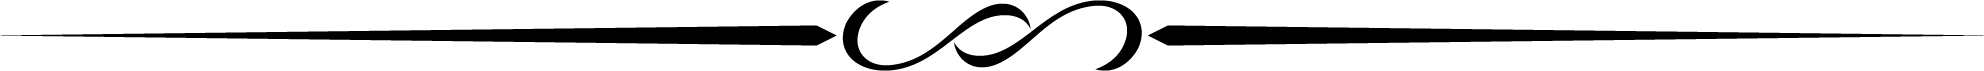
\includegraphics[width=0.4\linewidth]{cut-off_rule.png}
	\vspace{-5ex}
\end{center}

\pdfbookmark[1]{封底}{back}
\hfill {\Large $\mathfrak{The\ End}$ \Coffeecup}
\vspace{5.555ex}

% \clearpage
% \appendix

% \section{测试题}

% \subsection*{随堂 \normalfont\footnotesize (2021年10月25日)}
% \begin{Prob}
% 设$M = (M_{t})_{t \ge 0} \in \mathcal{M}^{2}_{\mathrm{cts}}$. 证明:
% \begin{enumerate}
% 	\setlength{\itemsep}{0ex}
% \item 若$0 \le t_{0} \le t_{1} < t_{2}$, 且$\xi_{1} \in L^{\infty}(\mathscr{F}_{t_1})$, 则$\E[\xi_{1}^{2}(M_{t_2}-M_{t_1})^{2}|\mathscr{F}_{t_0}] = \E[\xi_{1}^{2}(\agp{M}_{t_2}-\agp{M}_{t_1})|\mathscr{F}_{t_0}]$.
% \item 对于$X \in \mathcal{L}_{0}$, 有$\E[(I^{M}_{t}(X)-I^{M}_{s}(X))^{2}|\mathscr{F}_{s}] = \E[\tint_{u=s}^{t}X_{u}^{2}\d\agp{M}_{u}|\mathscr{F}_{s}] ~(\as)$, $\forall t > s$.
% \end{enumerate}
% \end{Prob}

% \begin{Prob}
% 设$N = (N_{t})_{t \ge 0}$是速率参数为$\lambda$的Poisson过程. 求$((N_{t} - \lambda t)^{2})_{t \ge 0}$的Doob--Meyer分解.
% \end{Prob}


% \setcounter{Prob}{0}
% \subsection*{随堂 \normalfont\footnotesize (2021年11月22日)}
% \begin{Prob}
% 叙述并证明L\'{e}vy的Brown运动鞅刻画.
% \end{Prob}

% \begin{Prob}
% 设$B = B^{1} + \sqrt{-1} B^{2}$是初值为$z \in D$的复标准Brown运动, $f : D \to \mathbb{C}$是非常值全纯函数, 其中$D$是$\mathbb{C}$的连通开子集. 设$\tau_{s}$满足$S_{\tau_{s}} = s$, 其中$S_{t} := \int_{0}^{t} \abs{f'(B_{r})}^{2} \d r$, $0 \le t < \epsilon_{D} := \inf\{ t : B_{t} \notin D \}$. 证明$f(B_{\tau_{s}})_{0 \le s < S_{\epsilon_{D}}}$是初值为$f(z)$的停止于$f(\partial D)$的复标准Brown运动.
% \end{Prob}


% \setcounter{Prob}{0}
% \subsection*{随堂 \normalfont\footnotesize (2021年12月20日)}
% \begin{Prob}
% 叙述并证明Cameron--Martin--Girsanov定理.
% \end{Prob}

% \begin{Prob}
% 证明Stroock--Varadhan鞅方法(定理\ref{Thm:Stroock--Varadhan})的充分性部分.
% \end{Prob}



% \setcounter{Prob}{0}
% \subsection*{期末 \normalfont\footnotesize (2021年12月29日)}
% 前6题选4道, 后4题选2道.
% \begin{Prob}[15']
% 叙述并证明Cameron--Martin--Girsanov定理.
% \end{Prob}
% \begin{Prob}[15']
% 考虑$X_{t} := \1_{\{t \ge T\}}$, $t \ge 0$, 其中给定随机变量$T > 0$. \par
% (1) 求Doob--Meyer分解. (2) 求二次变差. (3) 求$\int_{s=0}^{t} X_{s-} \d X_{s}$.
% \end{Prob}
% \begin{Prob}[15']
% 证明Stroock--Varadhan鞅方法(定理\ref{Thm:Stroock--Varadhan}).
% \end{Prob}
% \begin{Prob}[15']
% 求一个随机过程的局部时.
% \end{Prob}
% \begin{Prob}[15']
% 设$M$是连续局部鞅, 证明$\{ \agp{M}_{\infty} < \infty \} \stackrel{\as}{=} \{ \lim_{t\to\infty} M_{t} ~\text{存在且有限} \}$.
% \end{Prob}
% \begin{Prob}[15']
% 设$B = (B_{t})_{t \ge 0}$是标准Brown运动, $\phi : \R \to \R$有界. 求$\e^{\int_{0}^{T} \phi(B_{s}) \d s}$的It\^{o}积分表示.
% \end{Prob}
% \begin{Prob}[20']
% 证明平方可积连续鞅的二次变差的性质. (\cite{Karatzas-Shreve--GTM113}~1.5.8)
% \end{Prob}
% \begin{Prob}[20']
% 设$B = (B_{t})_{0 \le t \le 1}$是零初值标准Brown运动. 与$(B_{t}-tB_{1})_{0 \le t \le 1}$同分布的随机过程称为Brown桥. (1--4) 证明Brown桥有限维分布等同于$B\,|\,B_{1}=0$. \par (5--8) 证明$\d Y_{t} = \d B_{t} + \frac{Y_{t}}{t-1} \d t$的零初值强解存在唯一, 即$Y_{t} = (t-1) \int_{s=0}^{t} \frac{\d B_{s}}{s-1}$, 并且是Brown桥.
% \end{Prob}
% \begin{Prob}[20']
% 设$B = (B_{t})_{t \ge 0}$是零初值标准Brown运动, $f : \R \to \R$是光滑函数. 任给$\delta > 0$, 当$\varepsilon \to 0$时, (1) 证明$\P\{ \max_{t \in [0,1]} \abs{\varepsilon B_{t}} < \delta \} \to 1$; (2) 分析$\varepsilon^{2} \log \P\{ \max_{t \in [0,1]} \abs{\varepsilon B_{t} - f(t)} < \delta \}$渐近阶.
% \end{Prob}
% \begin{Prob}[20']
% 对于\eqref{eq:SDE}, 给一些条件后, 证明强解存在且唯一.
% \end{Prob}


\end{document}